% !TEX encoding = UTF-8 Unicode
%%%%%%%%%%%%%%%%%%%%%%%%%%%%%%%%%%%%%%%%%
% Masters/Doctoral Thesis 
% LaTeX Template
% Version 2.4 (22/11/16)
%
% This template has been downloaded from:
% http://www.LaTeXTemplates.com
%
% Version 2.x major modifications by:
% Vel (vel@latextemplates.com)
%
% This template is based on a template by:
% Steve Gunn (http://users.ecs.soton.ac.uk/srg/softwaretools/document/templates/)
% Sunil Patel (http://www.sunilpatel.co.uk/thesis-template/)
%
% Template license:
% CC BY-NC-SA 3.0 (http://creativecommons.org/licenses/by-nc-sa/3.0/)
%
%%%%%%%%%%%%%%%%%%%%%%%%%%%%%%%%%%%%%%%%%

%----------------------------------------------------------------------------------------
%	PACKAGES AND OTHER DOCUMENT CONFIGURATIONS
%----------------------------------------------------------------------------------------

\documentclass[
11pt, % The default document font size, options: 10pt, 11pt, 12pt
%oneside, % Two side (alternating margins) for binding by default, uncomment to switch to one side
english, % ngerman for German
onehalfspacing, % Single line spacing, alternatives: onehalfspacing or doublespacing
%draft, % Uncomment to enable draft mode (no pictures, no links, overfull hboxes indicated)
%nolistspacing, % If the document is onehalfspacing or doublespacing, uncomment this to set spacing in lists to single
%liststotoc, % Uncomment to add the list of figures/tables/etc to the table of contents
%toctotoc, % Uncomment to add the main table of contents to the table of contents
%parskip, % Uncomment to add space between paragraphs
%nohyperref, % Uncomment to not load the hyperref package
headsepline, % Uncomment to get a line under the header
%chapterinoneline, % Uncomment to place the chapter title next to the number on one line
%consistentlayout, % Uncomment to change the layout of the declaration, abstract and acknowledgements pages to match the default layout
]{MastersDoctoralThesis} % The class file specifying the document structure

%\usepackage[utf8]{inputenc} % Required for inputting international characters
\usepackage[T1]{fontenc} % Output font encoding for international characters
\usepackage{palatino} % Use the Palatino font by default
\usepackage{fontspec}
\usepackage[backend=biber,style=authoryear,natbib=true]{biblatex} % Use the bibtex backend with the authoryear citation style (which resembles APA)
\addbibresource{example.bib} % The filename of the bibliography
\usepackage[autostyle=true]{csquotes} % Required to generate language-dependent quotes in the bibliography
\usepackage[it]{subfigure}
\usepackage{graphicx}
\usepackage{listings}
\usepackage{changepage}
\usepackage{eso-pic}
\usepackage{multirow}
\usepackage{epigraph}
\usepackage{xcolor}
\usepackage{multirow}
\usepackage{colortbl}
%----------------------------------------------------------------------------------------
%	MARGIN SETTINGS
%----------------------------------------------------------------------------------------

\geometry{
	paper=a4paper, % Change to letterpaper for US letter
	inner=2.5cm, % Inner margin
	outer=3.8cm, % Outer margin
	bindingoffset=.5cm, % Binding offset
	top=1.5cm, % Top margin
	bottom=1.5cm, % Bottom margin
	%showframe, % Uncomment to show how the type block is set on the page
}

\makeatletter
\def\blx@maxline{77}
\makeatother

\newcommand\BackgroundPic{%
\put(0,0){%
\parbox[b][\paperheight]{\paperwidth}{%
\vfill
\centering
\includegraphics[width=\paperwidth,height=\paperheight,%
keepaspectratio]{Thesis.pdf}%
\vfill
}}}

\lstset{numbers=left,xleftmargin=2em,frame=lines,framexleftmargin=1.5em,stepnumber=1,basicstyle=\ttfamily,breaklines=true}
%----------------------------------------------------------------------------------------
%	THESIS INFORMATION
%----------------------------------------------------------------------------------------

\thesistitle{An open database model and Android database application for storing Obstructive Sleep Apnea data} % Your thesis title, this is used in the title and abstract, print it elsewhere with \ttitle
\supervisor{Prof. Dr. Thomas \textsc{Peter Plagemann}} % Your supervisor's name, this is used in the title page, print it elsewhere with \supname
\examiner{} % Your examiner's name, this is not currently used anywhere in the template, print it elsewhere with \examname
\degree{Master of Science} % Your degree name, this is used in the title page and abstract, print it elsewhere with \degreename
\author{Viet Thi \textsc{Tran}} % Your name, this is used in the title page and abstract, print it elsewhere with \authorname
\addresses{} % Your address, this is not currently used anywhere in the template, print it elsewhere with \addressname

\subject{Informatics} % Your subject area, this is not currently used anywhere in the template, print it elsewhere with \subjectname
\keywords{} % Keywords for your thesis, this is not currently used anywhere in the template, print it elsewhere with \keywordnames
\university{\href{http://www.uio.no/english/}{ }} % Your university's name and URL, this is used in the title page and abstract, print it elsewhere with \univname
\department{\href{http://www.mn.uio.no/ifi/english/}{Department of Informatics}} % Your department's name and URL, this is used in the title page and abstract, print it elsewhere with \deptname
\group{\href{https://www.mn.uio.no/ifi/forskning/grupper/dmms/}{Distributed MultiMedia Systems (DMMS)}} % Your research group's name and URL, this is used in the title page, print it elsewhere with \groupname
\faculty{\href{http://www.mn.uio.no/english/}{The Faculty of Mathematics and Natural Sciences}} % Your faculty's name and URL, this is used in the title page and abstract, print it elsewhere with \facname

\AtBeginDocument{
\hypersetup{colorlinks=false}
}

\begin{document}
\AddToShipoutPicture*{\BackgroundPic}
\frontmatter % Use roman page numbering style (i, ii, iii, iv...) for the pre-content pages

\pagestyle{plain} % Default to the plain heading style until the thesis style is called for the body content

%----------------------------------------------------------------------------------------
%	TITLE PAGE
%----------------------------------------------------------------------------------------

\begin{titlepage}
\begin{center}

\vspace*{.06\textheight}
{\scshape\LARGE \univname\par}\vspace{1.0cm} % University name
\textsc{\Large }\\[2.0cm] % Thesis type

{\huge \bfseries \ttitle\par}\vspace{0.4cm} % Thesis title
 
\begin{minipage}[t]{0.4\textwidth}
\begin{flushleft} \large
\emph{Student:}\\
\href{http://www.mn.uio.no/ifi/?vrtx=person-view&uid=viettt}{\authorname} % Author name - remove the \href bracket to remove the link
\end{flushleft}
\end{minipage}
\begin{minipage}[t]{0.4\textwidth}
\begin{flushright} \large
\emph{Supervisor:} \\
\href{http://www.mn.uio.no/ifi/personer/vit/plageman/index.html}{\supname} % Supervisor name - remove the \href bracket to remove the link  
\end{flushright}
\end{minipage}\\[4cm]
 
\vfill

\large \textit{A thesis submitted in fulfillment of the requirements\\ for the degree of \degreename}\\[0.3cm] % University requirement text
\textit{in the}\\[0.4cm]
\groupname\\\deptname\\[2cm] % Research group name and department name
 
\vfill

{\large \today}\\[4cm] % Date
%\includegraphics{Logo} % University/department logo - uncomment to place it
 
\vfill
\end{center}
\end{titlepage}

%----------------------------------------------------------------------------------------
%	DECLARATION PAGE
%----------------------------------------------------------------------------------------

%\begin{declaration}
%\addchaptertocentry{\authorshipname} % Add the declaration to the table of contents
%\noindent I, \authorname, declare that this thesis titled, \enquote{\ttitle} and the work presented in it are my own. I confirm that:

%\begin{itemize} 
%\item This work was done wholly or mainly while in candidature for a research degree at this University.
%\item Where any part of this thesis has previously been submitted for a degree or any other qualification at this University or any other institution, this has been clearly stated.
%\item Where I have consulted the published work of others, this is always clearly attributed.
%\item Where I have quoted from the work of others, the source is always given. With the exception of such quotations, this thesis is entirely my own work.
%\item I have acknowledged all main sources of help.
%\item Where the thesis is based on work done by myself jointly with others, I have made clear exactly what was done by others and what I have contributed myself.\\
%\end{itemize}
 
%\noindent Signed:\\
%\rule[0.5em]{25em}{0.5pt} % This prints a line for the signature
 
%\noindent Date:\\
%\rule[0.5em]{25em}{0.5pt} % This prints a line to write the date
%\end{declaration}

\cleardoublepage

%----------------------------------------------------------------------------------------
%	QUOTATION PAGE
%----------------------------------------------------------------------------------------

%\vspace*{0.2\textheight}

%\noindent\enquote{\itshape Thanks to my solid academic training, today I can write hundreds of words on virtually any topic without possessing a shred of information, which is how I got a good job in journalism.}\bigbreak

%\hfill Dave Barry

%----------------------------------------------------------------------------------------
%	ABSTRACT PAGE
%----------------------------------------------------------------------------------------

\begin{abstract}
\addchaptertocentry{\abstractname} % Add the abstract to the table of contents
Sleep apnea is a sleep disorder that causes repeatedly reduced respiration or no airflow in a period of time during sleep. Sleep apnea can be detected by analyzing bio-physiological signals such as electrocardiogram, oxygen saturation, and respiratory effort, etc. The bio-physiological signals that are recorded during sleep, are usually kept in files which have low level abstractions, indexing primitives, and diverse formats such as EDF/EDF+ file formats, or a Waveform Database format (PhysioBank databases). To manage and query data from these files the provided software packages are required, i.e. the WFDB software package for the Waveform Database format. Otherwise, it is necessary to write a new software application based on the specification of the file formats, which leads to increased difficulty of programming and analyzing bio-physiological data. The thesis presents design and implementation of a relational database model for storing not only Obstructive Sleep Apnea signals, but also other bio-physiological signals. The first benefit of using a relational database for storing bio-physiological data is that there is no need to write or include management tools for managing the collected data. Furthermore, data analysis can be directly performed on the collector devices (mobile devices) by using the SQL language, which provides many useful algorithms for analyzing data. In addition, remote services can ask for some parts of data from collector devices by using remote querying. Last but not least, the privacy of patients is not violated if they can keep their bio-physiology on their own devices, and can decide which data they would like to send. The database model that is presented is this thesis is a platform independent, it can therefore be implemented on whatever database management system as long as they support SQL language. In this thesis, a design and implementation of a database application for the database model are proposed. The design is discussed first at an abstract and platform independent level, in which it describes the ways the database application works with real-time sources and files. The Android platform is chosen as implementation platform for both the database model and database application. Data sources for the database are from the CESAR acquisition tool and EDF files that are exported from PhysioBank.\\
The database size is less than 1736 MB after collecting data from all channels of the CESAR acquisition tool with 100Hz for each channel in nearly 19 hours. That is, the application can collect data for a whole day without any storage problem. The power consumption for the application is 6.6\% of the total power drain on the device, which is quiet efficient. The average read time and write time are 17936 samples per second and 12960 samples per second. With a stress test, the application shows that it can manage all channels of 14 BITalino sensor kit with 100Hz while importing a EDF file, exporting data from six channels to a EDF file, and visualizing incoming samples on a graph.\\
Nevertheless, the results show that the database model and database application are very efficient for storing and analyzing Obstructive Sleep Apnea signals, and other bio-physiological signals.\\
\end{abstract}

%----------------------------------------------------------------------------------------
%	ACKNOWLEDGEMENTS
%----------------------------------------------------------------------------------------

\begin{acknowledgements}
\addchaptertocentry{\acknowledgementname} % Add the acknowledgements to the table of contents
First of all, I would like to thank my supervisor Professor Dr. Thomas Plagemann, who has conveyed a spirit of adventure in regard to scholarship and research to me, and provided invaluable insight through my thesis. Without his support and guidance, this thesis would not have been possible.\\\\
I would also like to thank my Norwegian teacher Marit Ruud McGhie, who constantly encouraged me in my early days in Norway. Without her encouragements, I could not pass the Norwegian course, and this thesis therefore might be done by someone else.\\\\
My sincere thanks also goes to the staffs and students at the Department of Informatics who contribute a friendly environment at the faculty, and thanks to my friends who have constantly blessed me in my daily work.\\\\
Special thanks to my family: my parents Tran Van Huu and Ngo Thi Xuan Huong for giving birth to me at the first place and supporting me spiritually throughout my life. I would also like to thank my brothers and sisters for providing me with unfailing support and continuous encouragement throughout my years of study and through the process of writing this thesis.\\\\
Last but not the least, I would like to thank my partner Vo Thi Hanh Nhan, who has been trusting and waiting for me for nearly 10 years. It's time to end the wating time.\\\
\epigraph{\hfill{\textit{Absence diminishes small loves and increases great ones, as the wind blows out the candle and fans the bonfire.}}}{\textbf{François de La Rochefoucauld}}
\end{acknowledgements}

%----------------------------------------------------------------------------------------
%	LIST OF CONTENTS/FIGURES/TABLES PAGES
%----------------------------------------------------------------------------------------

\tableofcontents % Prints the main table of contents

\listoffigures % Prints the list of figures

\listoftables % Prints the list of tables

\lstlistoflistings

%----------------------------------------------------------------------------------------
%	ABBREVIATIONS
%----------------------------------------------------------------------------------------

%\begin{abbreviations}{ll} % Include a list of abbreviations (a table of two columns)

%\textbf{LAH} & \textbf{L}ist \textbf{A}bbreviations \textbf{H}ere\\
%\textbf{WSF} & \textbf{W}hat (it) \textbf{S}tands \textbf{F}or\\

%\end{abbreviations}

%----------------------------------------------------------------------------------------
%	PHYSICAL CONSTANTS/OTHER DEFINITIONS
%----------------------------------------------------------------------------------------

%\begin{constants}{lr@{${}={}$}l} % The list of physical constants is a three column table

%The \SI{}{} command is provided by the siunitx package, see its documentation for instructions on how to use it

%Speed of Light & $c_{0}$ & \SI{2.99792458e8}{\meter\per\second} (exact)\\
%Constant Name & $Symbol$ & $Constant Value$ with units\\

%\end{constants}

%----------------------------------------------------------------------------------------
%	SYMBOLS
%----------------------------------------------------------------------------------------

%\begin{symbols}{lll} % Include a list of Symbols (a three column table)

%$a$ & distance & \si{\meter} \\
%$P$ & power & \si{\watt} (\si{\joule\per\second}) \\
%Symbol & Name & Unit \\

%\addlinespace % Gap to separate the Roman symbols from the Greek

%$\omega$ & angular frequency & \si{\radian} \\

%\end{symbols}

%----------------------------------------------------------------------------------------
%	DEDICATION
%----------------------------------------------------------------------------------------

%\dedicatory{For/Dedicated to/To my\ldots} 

%----------------------------------------------------------------------------------------
%	THESIS CONTENT - CHAPTERS
%----------------------------------------------------------------------------------------

\mainmatter % Begin numeric (1,2,3...) page numbering

\pagestyle{thesis} % Return the page headers back to the "thesis" style

% Include the chapters of the thesis as separate files from the Chapters folder
% Uncomment the lines as you write the chapters

\lhead{\emph{Introduction}}
\chapter{Introduction}
\section{Background and Motivation}
\section{Problem Statement}
 hope
\lhead{\emph{Sleep Apnoea}}
\chapter{Sleep Apnea}

Sleep apnea is a disorder where breathing stops and starts repeatedly during sleep. Stop breathing happens when either the airway collapses or the brain can not successfully send the signal to the breathing muscles. The first case is called Obstructive Sleep Apnea (OSA), and the second case is called Central Sleep Apnea (CSA). In both cases no air come in or out of the lung. It often lasts from a few seconds to minutes, and can happen about 30 times or more per hour\cite{NHLBI}. Sleep apnea is difficult to diagnose, because it happens when the patient sleeps. Moreover, sleep apnea can not be detected by normal tests such as blood test. It can be noticed by a family member when the patient intensively snores. However, CSA does not often come with snoring, therefore there it is difficult to detect sleep apnea in general. Sleep apnea can lead to many serious diseases if it is untreated, such as high blood pressure, heart attack, stroke, heart failure, etc. Getting not enough sleep can cause serious accidents if truck or taxi drivers have this disease. Section 2.1 presents a taxonomy of sleep apnea. Section 2.2 describes the physiological signals that can be used to diagnose sleep apnea.

\section{Taxonomy of sleep apnea}
Sleep apnea is more dangerous than people have thought, because it can lead to many other well-known diseases. According to The Akershus Sleep Apnea Project, there are 25\% middle-aged Norwegians at high-risk of having OSA\cite{Akershus}. That means sleep apnea is very common and it has to be studied seriously. In fact, there are dozen of research papers about it. When searching with "sleep apnea" on Google Scholar, it returns about about 18900 related articles. Sleep apnea is divided into three types:

\begin{itemize}
  \item OSA occurs when the soft tissue falls to the back of the throat which causes the breathing to be obstructed during sleep.
  \item CSA occurs when the brain fail to sends the signals to the breathing muscles and therefore it fails to control the breathing cycle.
  \item Mixed sleep apnea (MSA) is a combination of both OSA and CSA.
\end{itemize}

\subsection{Central sleep apnea}
    \textit{``Central sleep apnea syndrome is characterized by a cessation or decrease of ventilatory effort during sleep and is usually associated with oxygen desaturation."}\cite{Westchester}
    
    CSA happens when the brain can not send the appropriate signals to muscles which control breathing. CSA is not as common as obstructive sleep apnea. CSA is sometime a consequence of other diseases like heart failure, stroke, or sleep at high altitude.\\\\
    \textbf{Symptoms:} Common symptoms of CSA are awakening suddenly with breathlessnesses, insomnia, headache in the morning, difficulties to focus on work, hypersomnia, or snoring. The bed-partner can notice that the patient may stop breathing a number of times during sleep, about 30 times or more per hour, and the patient may snore. However, snoring is not common in CSA, and snoring does not always mean that a patient has sleep apnea.\\\\
    \textbf{Causes:} There are many causes that make the brain fail to connect with the breathing muscles. One of them is Cheney-Stokes, which is often associated with congestive heart failure or stroke, and is characterized by rhythmic cycles gradually increased and then decreased breathing which results in a temporary pause in breathing. 
    Other reasons which cause central sleep apnea are certain medical conditions. For example, if a patient has problem in cerebrovascular or has brain tumors can cause that signals to the breathing system get lost. Certain drugs such as opium, morphine or codeine can lead to irregular breathing like increase, decrease or stop breathing. Sometime sleep at high altitude can cause central sleep apnea, but it is not a big problem, because the problem will disappear when moving to a lower altitude.\\\\
    \textbf{Complications:} Not getting enough sleep can cause cardiovascular diseases. When the oxygen level in the blood is low, the heart will work hard to deliver blood to the tissues. If this lasts for a long time it may cause heart failure. Likewise, when the heart works hard, the pressure on the vascular increases which can cause hypertension. Hypertension is one of the most dangerous diseases and can lead to stroke or even dead. Waking up many times at night will make us tired and difficult to restore normal sleep. People who do not get enough sleep often have severe daytime sleepiness, fatigue and irritability. They can not focus on work and sometime fall asleep, not only at work but also when they drive a car.\\\\
    \textbf{Diagnostic methods:} Usually a doctor may perform an evaluation based on those symptoms which are mentioned above, or a patient must be sent to a treatment center for sleep disorders. At the treatment center, the patient can be analyzed by overnight monitoring breathing and other body functions during sleep. In polysomnography testing, the patient is connected to monitoring devices such as heart, lung, brain activity, breathing patterns, arm and leg movement, blood oxygen during levels sleep. Moreover, a review by a cardiologist or a doctor who specializes in the nervous system may also necessary to find the causes of central sleep apnea.\\\\
    \textbf{Treatments:} The first step of treatment is to try to cure the other diseases which cause the central sleep apnea. For example, a good treatment of a heart failure may eliminate central sleep apnea. The other way to treat this disease is to use drugs. There are some drugs which have been used to stimulate breathing for those who have central sleep apnea. For example, acetazolamide can be used to prevent central sleep apnea at high altitude. However, other drugs can cause apnea, for example opioid. The dose of opioid drugs need to be reduced if it causes central sleep apnea. However, drugs are not the major solution to treat central sleep apnea. \\There are four physical treatment methods which are often used in treating central sleep apnea. The first one is continuous positive airway pressure (CPAP), which uses mild air pressure to keep the airway open. This treatment is mainly used for obstructive sleep apnea where the patient wears a mask on the nose during sleep, but it is also used for central sleep apnea. Another useful method is bilevel positive airway pressure (BPAP) which supplies stable and continuous pressure in the upper airways while breathing in and out. BPAP provides high pressure when inhaling and low pressure when exhaling. The purpose of this treatment is to boost the weak breathing pattern of central sleep apnea into normal. Some BPAP devices can detect if there is no air-follow in a few seconds it will automatically active the breathing system. There is a better solution than CPAP and BPAP, that is called adaptive servo ventilation (ASV). ASV is designed to treat central sleep apnea and complex sleep apnea by monitoring normal breathing pattern and storing it in a database system as a training set. When the patient falls asleep, ASV monitors the breathing process and compares it with the training set. If there is apnea, ASV will use pressure to regulate the breathing pattern and prevent pause in breathing. The last method is using supplemental oxygen, but there are many arguments against this method. The main argument is that the oxygen level may normalize, but the carbon dioxide can not release. As a result, a signal will be sent to brain which causes awakenings and the sleep will be fragmented. 
\subsection{Obstructive sleep apnea}
    \textit{``Obstructive sleep apnea syndrome is characterized by repetitive episodes of upper airway obstruction that occur during sleep, usually associated with a reduction in blood oxygen saturation."}\cite{Westchester}
    
    Several types of sleep apnea exist, but the most serious and common type is obstructive sleep apnea. It occurs when the throat muscles relax and blocks the airway during sleep. The most noticeable signal of obstructive sleep apnea is snoring, although not everyone who snores has obstructive sleep apnea. It usually affects old people, but anyone can have this illness. Obstructive sleep apnea is particularly common for those who are overweight. We discuss more in detail about its symptoms, causes, complications, diagnostic methods, and treatments below.\\
    \textbf{Symptoms:} As mentioned above, the most common signs is loud snoring and sometimes pausing in snoring. When there is a pausing in snoring, choking and gasping may follow it. Apnea occurs when the throat muscles relax and block the airway, therefore when we sleep on our back the snoring will be loudest. When we turn on our side, the snoring sound will decrease or even stop. That explains why we do not snore every night. It is difficult for us to recognize that we are snoring. However, a family member can easily notice the problem. Another sign is that we have excessive sleepiness during the day, can fall asleep while working, watching television or even driving. When we do not have normal breathing at night, our brain does not have enough oxygen to work. It causes not only morning headaches, but also memory problems. The other good sign to detect obstructive sleep apnea is waking up with dry mouth or sore throat.\\
    \textbf{Causes:}
    The airway composes of mouth, nose, throat, and windpipe. It always opens under sleep when we do not have sleep apnea. 

    \begin{figure}[h]
        \centering
        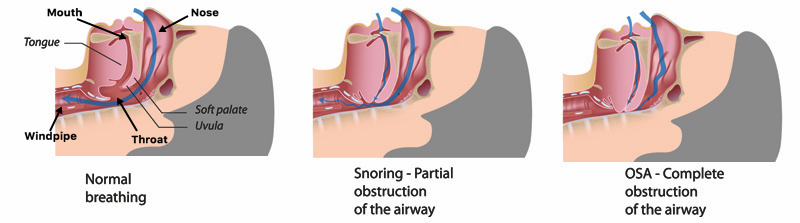
\includegraphics[width=1.0\textwidth]{Figures/ObstructionVentilationApnea.png}
        \caption{Obstructive Sleep apnea \cite{HudsonOSA}}
        \label{fig:Figures/ObstructionVentilationApnea}
    \end{figure}
    However, the airway becomes narrow when the soft palate and uvula relax. As a result, it is difficult to breath, and the patient might snore. This is called partial obstruction of the airway. When the muscles in the back of the throat relax too much, they will block the airway, as a result normal breathing is impossible. This situation is called complete obstruction of the airway, or obstructive sleep apnea. Blocked in breathing may cause a lower oxygen level in blood. Hence, the brain sends a signal to wake up the patient that the airway can be reopened. This process usually happens in a very short time and it is often not noticed because shortness of breath may be fixed with one or two deep breaths.\\ 
    Major causes of obstructive sleep apnea are old age, brain injury, decreased muscle tone, increased soft tissue around the airway, obese, or structural features that give rise to a narrowed airway\cite{OSAWiki}. Everyone can have obstructive sleep apnea, but certain factors imply a higher risk. The most significant factor is excess weight. Over a half of the people with OSA are overweight, because the fat of the upper respiratory can block breathing. The size of the neck may indicate whether someone at risk of OSA or not, because a thick neck can narrow the airway. Other risk factors are alcohol and smoking. Mihaela Trenchea et.al have researched on this topic and showed that smokers who smoke more than one pack  of cigarettes a day are at higher risk of severe obstructive sleep apnea than those who do not smoke\cite{ChestWorldCongress}. Other minor but not least causes are sex, age, genetic, or race. Overall, men are twice likely to develop OSA than women, and older have this illness more often than younger.\\
    \textbf{Complications:} Obstructive sleep apnea is a serious health problem which leads to several complications like:\\
    \textit{Cardiovascular diseases.} As mentioned in central sleep apnea complications, when the tissues do not get enough oxygen, the heart will beat fast and hard. As a result, the pressure on the heart and vascular will increase. About half of people with sleep apnea have high blood pressure, which increases the risk of heart failure and stroke. The more serious obstructive sleep apnea, the higher the risk of high blood pressure. With an underlying heart disease, a repeated low blood oxygen level can lead to sudden death from a cardiac event. Moreover, people with obstructive sleep apnea are often capable of developing abnormal heart rhythms like atrial fibrillation. \\\\
    \textit{Medications and surgery.} In general anesthesia, the doctor will use some medications like narcotic analgesics which can relax the patient's upper airway. When patient lies on his back, it will cause severe problems. Therefore it is important that patients with obstructive sleep apnea or related symptoms must inform the physician.\\\\
    \textit{Tired and sleepiness at daytime.} Similar to central sleep apnea, daytime drowsiness, fatigue and irritability are results from repeatedly awaking at night. Moreover, people with obstructive sleep apnea have often difficulties to focus on work or driving. Hence, it is not only dangerous for the patient, but also dangerous for people who are around him.\\\\
    \textit{Partner's insomnia.} Snoring may be a huge problem for those who have to listen to it. Sleeping with a snoring bed partner sometime is a nightmare, because the people who do not snore can be woken up by the snoring sound. As a result, the partner may get some health problem related to insomnia. In some cases, the partner may leave sharing room to find a quiet place to sleep, or even it is a cause for divorce.\\\\
    
    \textbf{Diagnostic methods:}
    The evaluation may usually be performed by observing signs and symptoms. Then some tests need to be done, such as measuring the neck or checking the blood pressure. The medical doctor may examine the back of the throat, mouth and nose to find out if there are any abnormalities. Further evaluation requires to stay overnight at a sleep center. At that place, breath and other body functions are monitored while the patient is sleeping.\\\\
    \textit{Sleep tests.} 
    A patient may be asked to stay at a clinic for monitoring the heart, lung, brain activity, body movements, breathing patterns, and blood oxygen levels during sleep by using professional devices. Based on the information from those sensors, the physician can diagnose obstructive sleep apnea and its level of severeness. Sometimes a patient has other diseases which also have the same symptoms as obstructive sleep apnea. For example, narcolepsy also causes excessive daytime sleepiness, but does not have the same treatment.\\\\
    \textit{Measuring oxygen.} 
    The patient does not need to come to a sleep center. Instead, a small sensor which can measure the oxygen level in blood can be used. The patient can stay at home and wear this sensor on his finger to carry out the measurement. It is very simple, consistent and painless. While the patient sleeps, the sensor collects the information about oxygen level, and may store it on a computer or smart phone. Then the data will be sent to the physician. Based on the pattern of oxygen level in blood, the physician can determine if the patient has obstructive sleep apnea, or the patient may be recommended a sleep test at a sleep center.\\\\
    \textit{Otolaryngology tests.}
    This is often performed when a patient snores too loud. As mentioned earlier, when someone snores, it does not mean that he has obstructive sleep apnea. However, over a half people who snore have this illness. Hence, examinations on the nose, mouth, throat, palate, and neck need to be carried out.\\\\ 
    \textit{Cardiopulmonary tests.} 
    These tests usually relate to the measurements of the air flow, the breath samples and the heart rate samples. By observing the heart rate and respiration from the abdomen and chest, the physician can determine whether the patient has obstructive sleep apnea or not. 

    \textbf{Treatments:} We can apply three types of treatments which are lifestyle changes, therapies, and surgery or other procedures \cite{MAYOCLINIC}.\\
    \textit{Lifestyle changes.}
    This is the first  treatment to try when OSA is diagnosed. Half of people who have obstructive problem are obesity, hence trying to loose weight is the first thing to do for the overweighted patients. Beside weight-loss, avoiding alcohol is helpful, since alcohol can also cause this illness. Therefore, one should not drink too much alcohol, especially several hours before bed \cite{MAYOCLINIC}. Obstructive problem is happened when the airway at the throat collapses. Therefore, it is better to lie on the side instead of lying on the back.\\\\
    \textit{Therapies.} The methods applied for central sleep apnea are also applied for OSA, normally are CPAP, BPAP and ASV.\\\\
    \textit{Surgery.}
    The goal of surgery is to remove the excess tissue from the throat which can collapse and block the airway. There are several surgical options: surgical opening in the neck, surgical removal of tissue, jaw surgery, upper airway stimulation, and implants \cite{MAYOCLINIC}.
\subsection{Mixed sleep apnea}
    Mixed sleep apnea is also known as complex sleep apnea. It is a merger of central sleep apnea and obstructive sleep apnea. It is identified by researchers at Mayo Clinic \cite{ScienceDaily}. Mixed sleep apnea is caused when the respiratory control is interfered. Namely, the brain sends a signal to control the breathing system, but the responses of the breathing are not as the brain desired. When using CPAP, it can cause chaos on the ventilator control. As a result, obstructive sleep apnea can be cured, but the central sleep apnea can occur because the signals which are sent to the breathing system do not work. New CPAP devices can supply additional carbon dioxide to stabilize the breathing pattern to avoid mixed sleep apnea \cite{Hindawi}.
\section{Observable characteristics of obstructive sleep apnea}

    By examining the sensors' abilities of observing the signals which can be used to observe obstructive sleep apnea, we suggest to divide those signals into two categories. The first group comprises signals that can be simply measured by sensors which are integrated in smart wearable devices. The other group includes complex signals which can only be obtained by professional devices and can be transfered to user devices. Simple signals are the heartbeat, the change the volume of the chest and abdomen, and snoring. The complex signals include EEG, EMG, EOG, ECG, oxygen saturation in the blood, breathing, and blood pressure. Some non-professional devices can also obtain these signals. However, the results from them are not good enough to use for medical diagnosis. For instance, the BITalino can observe almost all of the complex signals, but it is not a medical device as disclaimer on the BITalino website.

    \begin{figure}[h]
        \centering
        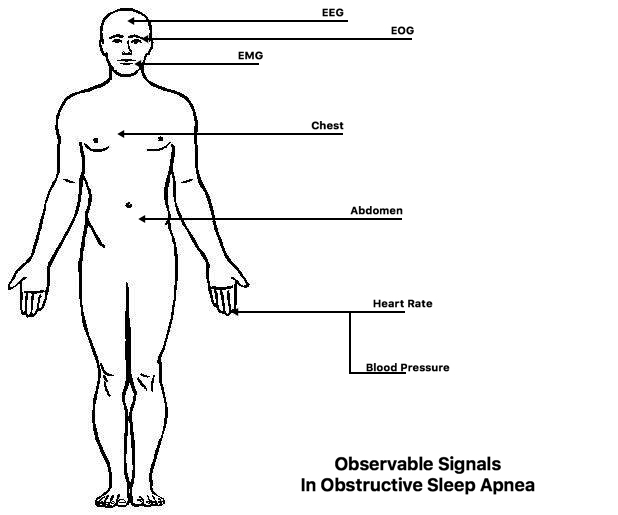
\includegraphics[width=1.0\textwidth]{Figures/humanbody.jpg}
        \caption{Observable Signals \cite{Advan}}
        \label{fig:Figures/humanbody}
    \end{figure}

    
    \textbf{Heartbeat. } The normal heart rate of a person varies from 60 to 100 beats per minute \cite{HEARTORG_HR} depending on how often that person trained. Hence, each person has a stable heart rate in this range. However, sleep apnea causes the heart rate to increase and to break the ordinary pattern. Heart rate is usually easily measured by using a smart watch or smart ring, or even a tattoo circuit. These devices can collect data and may send it to a smart phone to analyze it.

    \textbf{Snore. } Snoring can be measured by the microphone of a smart phone. The received signal is compared with available data samples. The result of the comparison can be used to determine whether the snoring is related to OSA or not. Snoring is often stopped after a period of time when people awake and start snoring again.

    \textbf{Measure the volume of air to breathe.} When observing the movement of the chest with a camera phone, Reyes gave Bersain\cite{BersainReyes} can calculate the average respiratory rate and tide volume.

    In addition to the signals which can be measured by integrated sensors on the smart devices, we can keep track of OSA by using non-integrated sensors to measure signals such as electroencephalogram (EEG), electromyography (EMG), electrooculography (EOG), electrocardiography (ECG), oxygen saturation in the blood, nasal airflow, and blood pressure.\\

    \textbf{EEG. } Wafaa S. Almuhammadi et.al\cite{IEEEOSAEEG} have done research on using EEG to classify OSA. They used EEG signals from Physionet as input for mining methods to detect if OSA exists or not. However, using only EEG for detecting OSA is not a good idea, because there are many health problems that have similar symptomatology to OSA, and one of them is epileptic \cite{NCBIEGEPILEPSY}. EEG can be recorded by placing the electrodes along the scalp, which is uncomfortable compared to wearing smart devices. However, EEG is very useful in combination with the others observable signals. In other words, EEG is considered an important signal for detecting OSA.\\\\
    \textbf{EMG. }People with OSA usually have longer time for the tongue to be recovered from relaxed. By examining the genioglossus muscle activity useful data for OSA diagnosis can be collected. Marc B Blumen et.al \cite{SDEMG} have found that those with OSA have tongue recovery time much longer than normal people after a constant submaximal effort, and they also have a smaller decrease in genioglossus muscle median frequency during effort. For OSA, we focus only on the signals from the tongue and genioglossus muscle because it causes the airway to be blocked. Other EMG signals are not considered, because they are not relevant.\\\\
    \textbf{EOG. }To measure eyes movements during sleep electrooculography is used. Electrooculography has two electrodes. The front of the eyes, also known as the cornea, is electrically positive while the back, also known as the retina, is electrically negative. Therefore, it is possible to measure the variation in voltage to determine the movements of the eyes. Rapid eye movement (REM) is a factor in the occurrence of disordered breathing events\cite{JSREM}. \\\\
    \textbf{ECG. } ECG presents the electrical activity of the heart, and it is one of the most efficient signal to detect OSA. By placing the electrodes on the skin, the tiny electrical changes on skin during each heartbeat can be detected. Laiali Almazaydeh et.al \cite{RESEARCHGATE} have done research on detecting OSA by using ECG signal features. They observe the wave forms from ECG, then identify an R peak. Once R peak is identified, they calculate RR intervals. After extracted, RR intervals are submitted to SVM in order to do classification.\\\\
    \textbf{Oxygen saturation. } Oxygen saturation can be measured by using pulse oximetry. Pulse oximetry is a noninvasive and inexpensive procedure which is used to measure the level of oxygen in blood. It is very simple to make measurements, a clip-like sensor can be placed on the earlobe, nose or fingers\cite{WIKIHOW}. The level of oxygen in the blood is usually above 95\%.\\\\
    \textbf{Nasal airflow. } Airflow sensors can measure the air pressure in nose when inhaling and exhaling. The sensor can be easily placed, but it is uncomfortable to wear it during sleep. A lot of studies have reported that it is not a good signal for detecting OSA, but it is still used\cite{HINDIWAAIRFLOW}. Therefore, we consider nasal airflow as one of signals to detect OSA.\\\\
    \textbf{Blood pressure. } Blood pressure can be measured by a simple, noninvasive sensor. This sensor can easily clip on the finger. According to American Heart Association\cite{HEARTORG}, the normal blood pressure with systolic is less than 120 mm Hg, and with diastolic is less than 80 mm Hg. Getting higher number than these numbers when sleeping is considered having OSA. As explained in OSA causes, the pressure is high when the breathing pauses.\\


 
\chapter{Data sources and data formats}
Signals for OSA come from many different sensor data sources. Moreover, the quality of these signals is diverse. Signals that come from clinical grade sensors are used in the medical domain, while signals that come from consumer electronic sensors are often used for fitness trackers, research, etc. In other words, consumer electronic sensors are not allowed in medicine, because they have not been approved yet. Therefore, a hypothesis is made that the signals from clinical sensors have better quality than the consumer electronic sensors. This chapter presents two corresponding sensor data sources for these two types of sensors. Consumer electronic signals come from BITalino sensors while clinic grade signals are stored in the Physionet database and captured with clinical grade sensors. In addition, different sensor data sources provide different formats to obtain and store the signals. Therefore, this chapter also presents a description of data formatting for each of the sensor data sources. In Section 3.1, an overview of data sources is presented. Section 3.2 presents different methods to format data signals. Standard formats, which are the European Data Format (EDF)\cite{EDF1} and the European Data Format plus (EDF+) are presented in Section 3.2. Section 3.3 presents two data acquisition tools that can be used to obtain biosignals from sensor sources.
\section{Data sources}
    In general, the quality of data has a huge influence to the data analysis process. Better analysis results are often derived from a higher quality data source. Therefore, choosing a good data source is vital for analyses. Misleading results are caused by various reasons, and a low quality data source is one of the major causes. However, a good source often comes with a very expensive price. In medicine, for obtaining biosignals has to follow strict requirements, and often use expensive clinical grade sensors to harvest these signals. The clinical data sensors provide high quality signals which can create a high quality dataset. After all, it is much more expensive to buy and maintain a clinical sensor system than a consumer electronic sensor system. For example, a NOX-T3 from nox-medical costs 55000kr plus value added tax\cite{Thomas} while a BITalino costs about 1000kr. The consumer electronic sensors often come with reasonable or even low price, because the quality of signals have not been approved, or maybe they are not good as the signals from the clinical sensors. However, there are many publications on using the consumer electronic sensors each year (for the BITalino 14 publications in 2015 and 7 publications in 2016\cite{BITalinoPubs}). Hence, an assumption is made that the quality of signals which is provided by the consumer electronic sensors is good enough to do research, build commercial applications etc. Nevertheless, the quality of biosignals and the support from consumer electronic sensors are promised to be improved in the future, because many leading companies constantly searching and integrated health care into their products, for example: Google Fit, Apple Health and Fitness, Microsoft band and Microsoft health, Xiaomi band, etc. This section presents an overview of BITalino which is one of the consumer electronic sensor groups for biosignals that has been used widely in many projects, products and researches, and Physionet database as clinical grade sensors source.
    \subsection{Data from BITalino sensors}
        BITalino is one of the reasonable priced sensor hardware platform which is easy to use and configure. BITalino is marked as DIY which means "do it yourself", therefore the goal of it is to use it for building an all-in-one platform such that every one can easily create their own biomedical devices. It is easy to configure, because BITalino is a plug-and-play device. The pre-conditioned analog outputs are sent wirelessly via bluetooth. Moreover, there are dozen of free, open source and paid softwares that support the BITalino sensor kit. These softwares can run on various operating systems, for example Linux, OSX, Windows, Android etc. Nevertheless, BITalino is not a medical device or to be used in medical diagnosis as they mentioned in their disclaimer on the website \cite{BITalino}. It is for students, teachers, researchers, etc., who do not need to have any engineering electrical skills to use it.
        \subsubsection{BITalino Kit}
            BITalino has a wide rang of sensors. Those sensors have the capability to measure either bio-electrical or bio-mechanical signals. BITalino has three major components that together form a basic bio-harvesting device. The first component is the power management which provides and manages power for biosignals acquisition. The BITalino power component uses a 3.7V LiPo battery to power its analog and digital parts. The second component is the micro controller unit (MCU) which is designed for accurate and reliable real-time streaming. It can control up to 6 analog inputs, 1 output, 2 digital inputs and 2 digital outputs at up to 1kHz \cite{BITalino_MCU}. The third component is data transfer. Data transfer is either bluetooth (BT) or bluetooth low energy (BLE), and is a ready-to-use module. The rest of the components are organized as independent modules that can be attached to the main board on demand.
            
            BITalino provides three kits: BITalino (r)evolution board, BITalino (r)evolution freestyle and BITalino (r)evolution plugged.\footnote{The evolution version is discontinued. The next generation of the BITalino is revolution, it has almost 2x the blocks and up to 60\% smaller sensors.}\\
            \begin{figure}[ht]
                \centering
                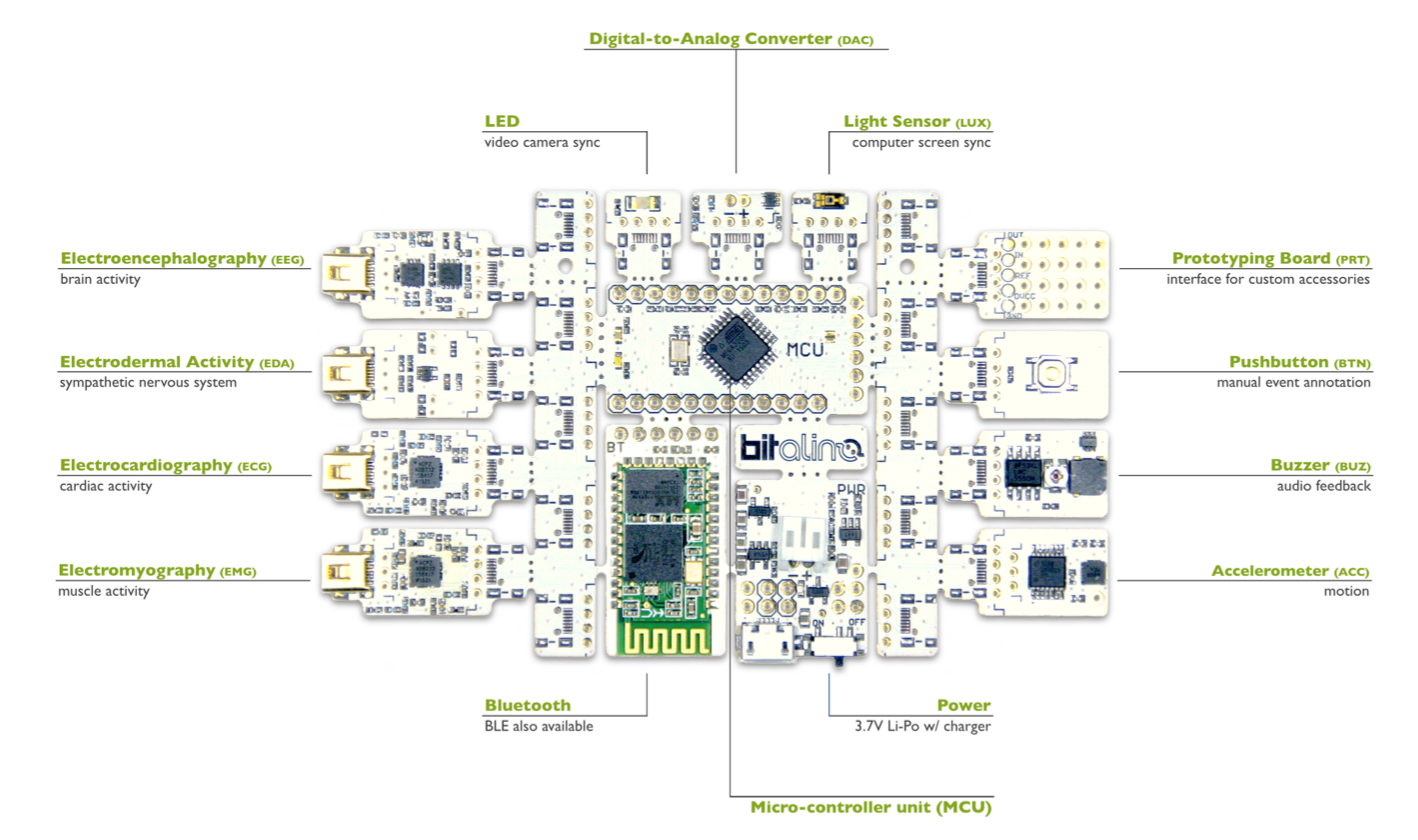
\includegraphics[width=1.0\textwidth]{Figures/BITalino_board.png}
                \caption{BITalino (r)evolution Board with Bluetooth connectivity \cite{BITalino_board}}
                \label{fig:Figures/BITalino_board}
            \end{figure}\\
            Figure 3.1 illustrates the BITalino (r)evolution board\cite{BITalino_board}. The size of the board is 100x65x6mm, and it is powered by a 3.7V recharge battery. The board consists of analog ports (4in - 10bit, 2in - 6bit, 1in - battery, 1out - 8bit) and digital ports (2in - 1bit, 2out - 1bit). In addition, it has either BT or BLE which have a range about 10m. There are seven sensors which are integrated on the board. They are electromyography (EMG), electrocardiography (ECG), electro-dermal activity (EDA), electroencephalography (EEG), accelerometer (ACC), light (LUX) and pushbutton (BTN). The board kit is designed as all-in-one device. The board connects all the necessary components which are the power management, MCU, BT and sensors into one board which is ready to use. This kit is made for biosignal exploration and lab activities. In conjunction with the OpenSignals software, it provides real-time biosignal data visualization.\\
            \begin{figure}[ht]
                \centering
                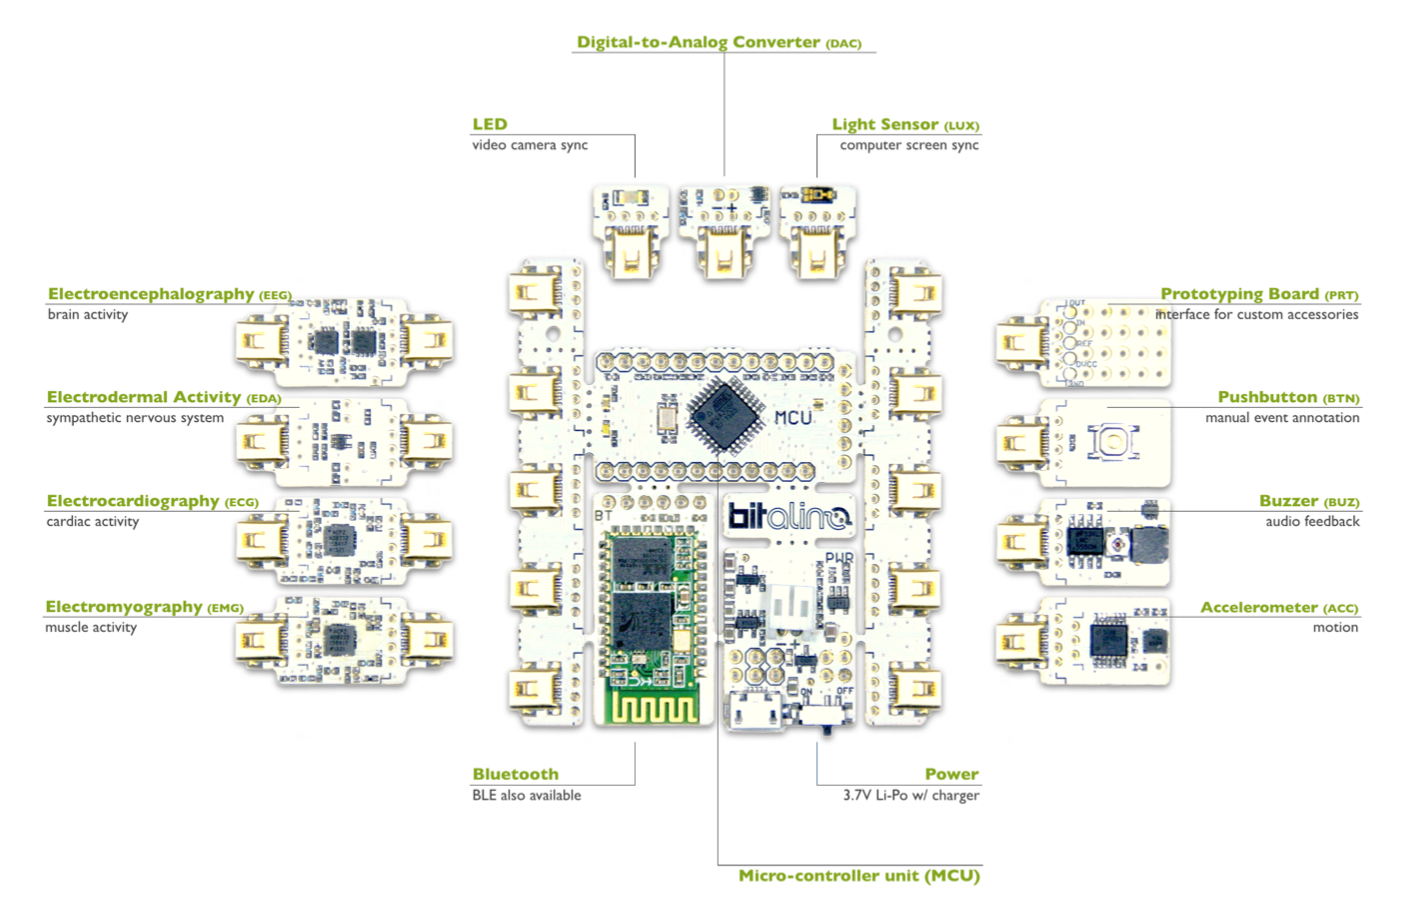
\includegraphics[width=1.0\textwidth]{Figures/BITalino_plugged.png}
                \caption{BITalino (r)evolution Plugged with Bluetooth connectivity \cite{BITalino_plugged}}
                \label{fig:Figures/BITalino_plugged}
            \end{figure}\\
            Figure 3.2 illustrates the BITalino (r)evolution plugged\cite{BITalino_plugged}. It is similar to the board kit, however the main board contains only three major components which are power management, MCU and BT. The main board also provides analog and digital ports to the inputs and outputs. The sensors do not integrate on the main board, they are separated from the board and connected as plug and play on demand. Therefore, the plugged kit provides maximum flexible configuration.\\
            \begin{figure}[ht]
                \centering
                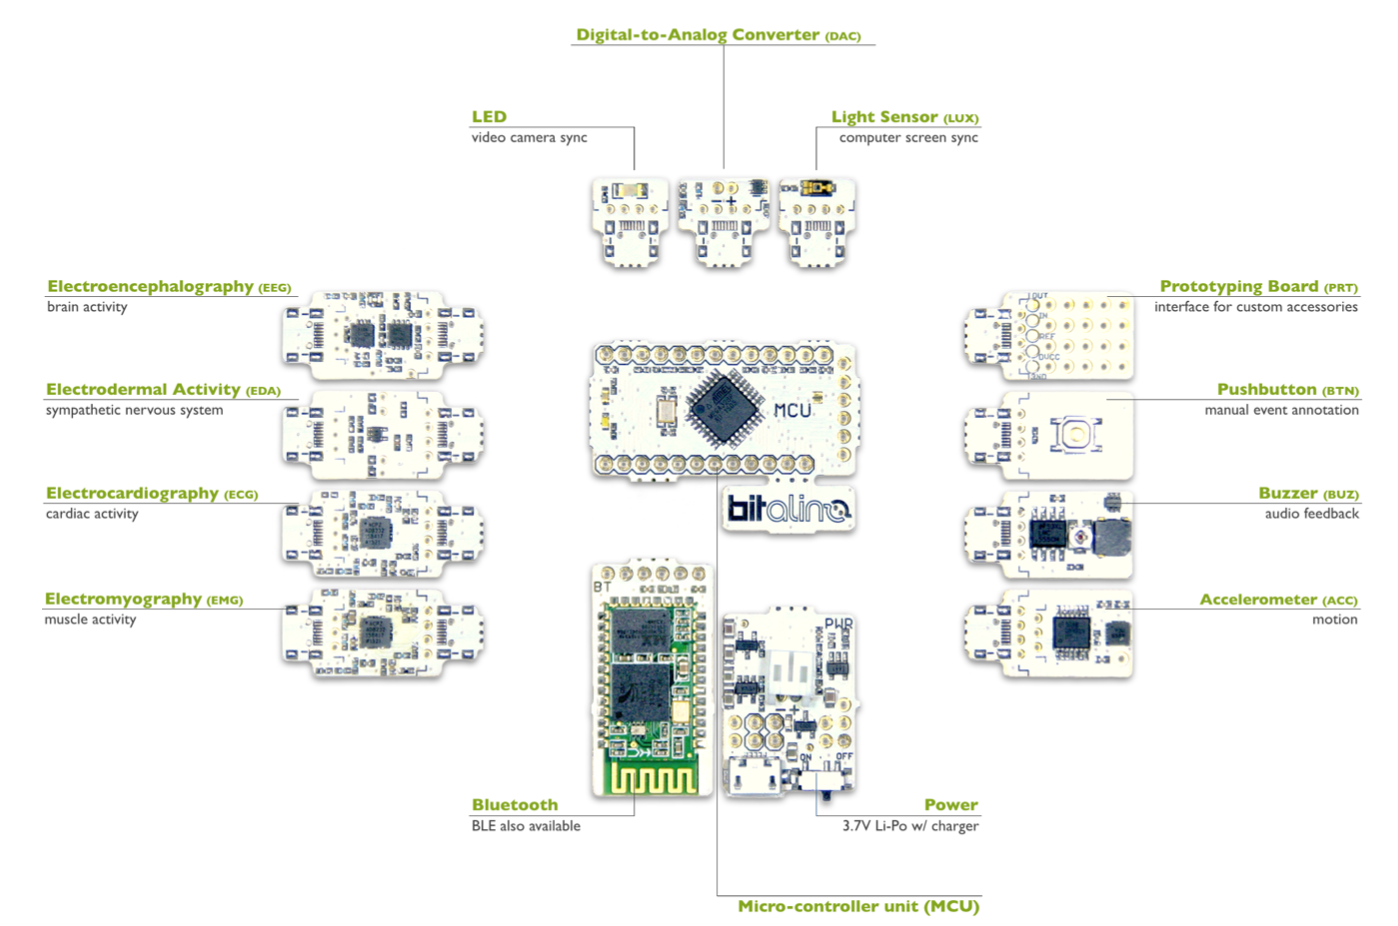
\includegraphics[width=1.0\textwidth]{Figures/BITalino_Freestyle.png}
                \caption{BITalino (r)evolution Freestyle with Bluetooth connectivity \cite{BITalino_Freestyle}}
                \label{fig:Figures/BITalino_Freestyle}
            \end{figure}\\
            Figure 3.3 illustrates the BITalino (r)evolution freestyle\cite{BITalino_Freestyle}. As the name of the kit, it provides maximum configuration. Hence, the users can maximize their imagination in building wearable biosignal acquisition devices. Each component is separated in a individual module, even the power management, MCU and BT are not on the same board.\\
        \subsubsection{BITalino sensors}
            This section briefly describes the sensors, i.e., EMG, ECG, EDA, EEG, ACC, LUX, BTN, PZT, that are provided by BITalino.\\
            The ACC sensor translates the motion into numerical values. BITalino provides 3-axis sensing for detecting tilt, monitoring activity, and measuring vibration. The sensor is limited in acquiring data from bio-mechanical and kinematic events. The sensor can be used in detecting posture, fall or shock, estimating rang of motion, step counting etc. Although it has 3 axis sensing, only the Z-axis is connected by default. It is because three analog outputs can be accessed separately, and the user can easily connect the X-axis and the Y-axis as their project demands.\\
            The ECG sensor translates the bio-electrical signals, which are low amplitude and generated by a set of cells in the heart, into numerical values. The ECG sensor from BITalino can obtain data not only at the chest, but also at the hand palms. Furthermore, the sensor works with pre-gelled electrodes as good as most types of the dry onces. According to ECG sensor data sheet, the sensor provides bipolar differential measurement with pre-conditioned analog output, and has a small form factor, and high signal-to-noise ratio. Therefore, it is widely used in heart rate and heart variability applications.\\
            The EDA sensor translates the resistance of the skin into numerical values. The human body secretes sweat not only when the body needs to regulate temperature, but also when the sympathetic nervous system activity is affected, for example when relaxing or arousing. The BITalino EDA sensor provides pre-conditioned analog output with high signal-to-noise ratio from measuring skin resistance. This signal is widely used in many applications such as lie detector, relaxation etc. and in this thesis it is used for detecting arousal and emotional cartography.\\
            The EMG sensor translates the bio-electrical signals which are sent from motor control neurons in the brain to the muscle fibers. A BITalino EMG sensor works with both dry and pre-gelled electrodes. This sensor has a wide range of applications such as muscle reflex studies, nerve conduction measurement, human-computer interaction etc.\\
            The LUX sensor translates the intensity of light into a digital signal. The BITalino LUX sensor can be adapted to human eye responsiveness.\\
            The push button is useful for taking the annotation of meaningful events which occur during the observation.\\
            BITilano TMP sensor translates the temperature of a body or the environment into digital values which range from -40C to +125C. The accuracy of the sensor varies from -2C to +2C, and the linearity is 0.5. It is small (about 12x27mm) and has low power consumption (about 0.05mA) which are good properties for building wearable devices.\\
            PZT sensor translates the displacement variations induced when inhaling or exhaling into numerical values. BITalino PZT sensor consists of a adjustable chest strap, RJ22 connector and a sensor which is secured in the chest strap. A BITalino PZT sensor is a good option for respiratory analysis.
        \subsubsection{Logical sensors}
            A sensor network consists of dozens of sensor. Sometimes some of them need to be taken down for maintenance, or the network needs to integrate additional sensors to form a bigger network. A methodology has been introduced by C.Hansen et.al\cite{LOGICALSENSOR_1} in November 1983 to deal with the problem, which is a logical sensor. The overall goal of logical sensors is to aid in the coherent synthesis of efficient and reliable sensor systems. There are two problems regarding to sensor systems\cite{LOGICALSENSOR_0}. The first problem is how to build an efficient and coherent method for the information provided by various kinds of sensors. The second problem is how to maintain and develop the system for that it can be incorporated with additional sensing devices. Sensor data abstraction is introduced for solving these problems. Data abstraction techniques are used to analyze and create patterns (logical sensors) from sensor data\cite{SensorDataAbstract}. The patterns are considered the interfaces for sensor systems which make the systems easily to be reconfigured in the future. Furthermore, the patterns together with the sensor semantic descriptions help to minimize the size of the data which is sent from the sensor nodes to the gateways or high level processing components. There are many principle motivations for logical sensor specification. Three of them are emergence of multi-sensor systems (a coherent data acquisition and integration system is needed), benefits of data abstraction (an inherent hierarchical structuring of logical sensors further aids system is needed) and availability of smart sensors (substitution of hardware for software and vice versa)\cite{LOGICALSENSOR_3}.
    \subsection{Physionet sensor databases}
        As mentioned earlier, the quality of data plays a very important role in choosing data sets. Especially for biosignals, the data must be from the trustworthy sources. Therefore, Physionet sensor databases are chosen as trustworthy clinical grade sources. Physionet is inaugurated by the researchers at Boston's Beth Israel Deaconess Medical Center, Boston University, McGrill University and MIT\cite{PhysioNet_Intro}. To date it is supported by the National Institute of General Medical Sciences and the National Institute of Biomedical Imaging and Bioengineering. Physionet has three interdependent components which are PhysioNet, PhysioBank and PhysioToolkit. The first component is PhysioNet which is used for exchanging and disseminating the biomedical signals and the software used to analyze those signals. PhysioNet also offers training opportunities\cite{PhysioNet_Training} that consist of tutorials on a variety of topics, special designed data sets for classroom activities and annual open challenges. PhysioBank is the second component which contains biosignal databases from various kind of diseases. PhysioBank unceasingly grows in both size and scope, to date even signals from vivo and vitro experiments are accepted \cite{PhysioNet_Contributing}. The last component is PhysioToolkit which provides tools for analyzing the biomedical signals. There are four databases in Physionet that can be used for analyzing OSA. They are apnea-ECG database, St. Vincent's University Hospital database, MIT-BIH polysomnographic database and SHHS polysomnography database.\\
        \textbf{Apnea-ECG database\cite{Apnea_ecg_db}: }\\
        This database has been created for Computers in Cardiology Challenge 2000 (CinC Challenge 2000). It was provided by Dr. Thomas Penzel of Phillipps-University, Marburg, Germany\cite{CinC2000}. The data consist of 70 records that are equally divided into two data sets. One is a learning set, the other is a test set. Each record has a 100 Hz with 12-bit resolution ECG signal which is digitalized and lasts for slightly less than 7 hours to nearly 10 hours. In addition, the record also contains a set of apnea annotations. The apnea annotations are marked by physicians whether an apnea event happens or not, one annotation per minute. However, the apnea annotations are not available in the test set due to the challenge, but are made available after the contest. The annotations include age, gender, height, weight, apnea index, hypopnea index and apnea-hypopnea index. Eight records which are called a01 to a04, b01 and c01 to c06 have extra four additional signals\cite{Apnea_ecg} for chest and abdominal respiratory effort, oronasal airflow, oxygen saturation in which the oxygen saturation signal digitized at 1Hz while the rest digitalized at 20Hz. Those additional signals are used as learning material to study the relationships between the respiration and ECG signals.\\
        These records are harvested between 1993 and 1999 \cite{Apnea_ecg_db}. During 1998 to 1999, the ECGs were digitized at 200Hz. However, to synchronize with the ECGs which are taken during 1993 and 1995, the newer ECGs were decimated to 100Hz. Therefore all records in the data set have 100Hz ECG signal. The signals are from three groups of subjects: the apnea group, the "borderline apnea" group and the normal group. The mean age of these three groups is slightly different, the higher the mean age, the more severe the apnea. Furthermore, due to lack of episodes of pure central apnea or of Cheyne-Stokes respiration, obstructive and mixed apnea can not be distinguished in this data set, this is to say a hypopnea minute is the same as an apnea minute. Nevertheless, the Apnea-ECG database is a good source to use for studying and doing research on sleep apnea.\\
        \textbf{St. Vincent's University Hospital database: }\\
        St. Vincent's University Hospital Sleep Disorders Clinic has collected 25 full overnight polysomnograms records with three-channel Holter ECG. The clinical and demographic information were at first collected and assembled under the guidance of professor Walter McNicholas, Dr. Liam Doherty, Dr. Silke Ryan and Dr. John Garvey, then scored and annotated by Ms Patrica Boyle, finally anonymized and electronic ally archived by Eric Chua. Signals which are monitored and stored are EEG, left EOG, right EOG, submental EMG, ECG, oronasal airflow, ribcage movements, abdomen movements, oxygen saturation, snoring and body position. The EDF format is used to save the records. Monitored subjects are above 18 years old, and randomly selected from patients referred to the clinic for that no known diseases can interfere with the heart rate. As a result, there are 25 subjects selected, i.e., 21 males and four females with the age range from 28 to 68 years, and the measured AHI range from 1.7 to 90.9\cite{STVinceUniversity}.\\
        \textbf{The MIT-BIH polysomnographic database: }\\
        The MIT-BIH polysomnographic database contains 16 subjects with sleep apnea syndrome from 60 male subjects in the age range of 32 to 56 years and a weight range from 89kg to 152kg\cite{MIT_BIH_slpdb}. This database is made for researchers who want to investigate clinical physiology, for engineers who want to develop a new method to analyze the digitized polysomnography data, and for students who want to learn sleep physiology. These subjects were observed in Boston's Beth Israel Hospital Sleep Laboratory for evaluating and testing CPAP. The monitored signals under observation are ECG, BP, EEG, Resp, EOG, EMG, SV and SO2 which have a sampling rate of 250Hz with 12-bit resolution. The recording time for each subject lasted from two to seven hours. This database is one of the most trustworthy resources for investigating and learning.\\
        \textbf{The SHHS polysomnography database: }
        The Sleep Heart Health Study polysomnography database is used for determining the relationship between cardiovascular diseases and other consequences of sleep-disordered breathing. From 1995 to 1998, 6441 men and women with the mean age of 40 took part in the sleep-related breathing examination\cite{SHSH_SleepData}. The participants can stay at their home under extermination, and are monitored by trained technicians. The recoded signals include EEGs at 125Hz, EOGs at 50Hz, EMG at 125Hz, thoracic and abdominal movements at 10Hz, nasal-oral airflow at 10Hz, finger-tip pulse oximetry at 1Hz, ECG at 125Hz, heart rate at 1Hz, body position and ambient light. There is only one polysomnogram sample which is formated in the EDF form available in Physionet. However, more data can be downloaded freely via the National Sleep Research Resource website\cite{SHSH_NationalSleepData}. Since this database was made by a multi-center cohort study which are supported by the National Heart Lung \& Blood Institute, it is also considered one of the most trustworthy resources for investigating and learning.
\section{Data formats}
    When collecting signals, the selection of a structure for storing data is very important issue. The selected structure must provide fast accessing, support cross platform, extensibility, multi modality, querying etc. In other words, this selection depends on the experiences of expert groups in implementing projects, the quality and the performance of the final result. Therefore, each group has its own data format for its special tasks. After choosing the data format, a set of rules are provided such that the database can be used outside the group. The problems raise when the number of groups increases. Hence, a standardized data format for biosignals is very essential for that these bio-research groups and clinics can not only coordinate and share data in an efficient way, but they can also improve the quality of the software.\\
    \subsection{Physionet sensor database formats}
        Although the stored data in the previously described four databases are biosignals, the format for each database is different.\\
        \textbf{Apnea-ECG database: }\\
        Apnea annotations are stored in the .apn and .qrs files\cite{Apnea_ecg_annotation}. In the .apn files, a one-minute interval is used between annotations. A "A" annotation presents that apnea was in progress at the beginning of the fellowed minute while a "N" annotation shows that apnea was not in progress at the beginning of the fellowed minute. Rdann\footnote{Rdann is a program that reads and converts the binary annotations files into text, one annotation per line.} needs to be used for converting the binary annotations in these files into text for viewing. However, the .qrs files can be viewed by using sqrs125\footnote{sqrs125 is a program that locates QRS complexes in an ECG signal in the specified record.}. In the .qrs files, all observed heart beats are marked with "N" annotations, and QRS-like artifacts are marked with "\textbar" annotations\cite{Apnea_ecg_annotation}.\\
        \textbf{St. Vincent's University Hospital database: }\\
        Unlike the way Apnea-ECG database stores its annotations (encoded its annotations), St. Vincent's University Hospital database has the annotations in a text file, the *\_stage.txt and *\_respevt.txt files. Figure 3.4 presents two tables for annotations in these files:
        \begin{figure}[ht]
        \centering     %%% not \center
        \subfigure[Annotations for *\_stage.txt\cite{STVinceUniversity_ann}]{\label{fig:VUH_ANN_S}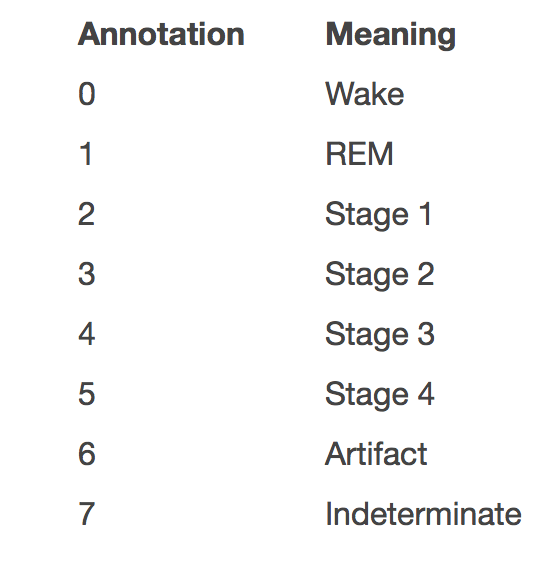
\includegraphics[width=50mm]{Figures/VUH_ANN.png}}
        \subfigure[Annotations for *\_respevt.txt\cite{STVinceUniversity_ann}]{\label{fig:VUH_ANN_R}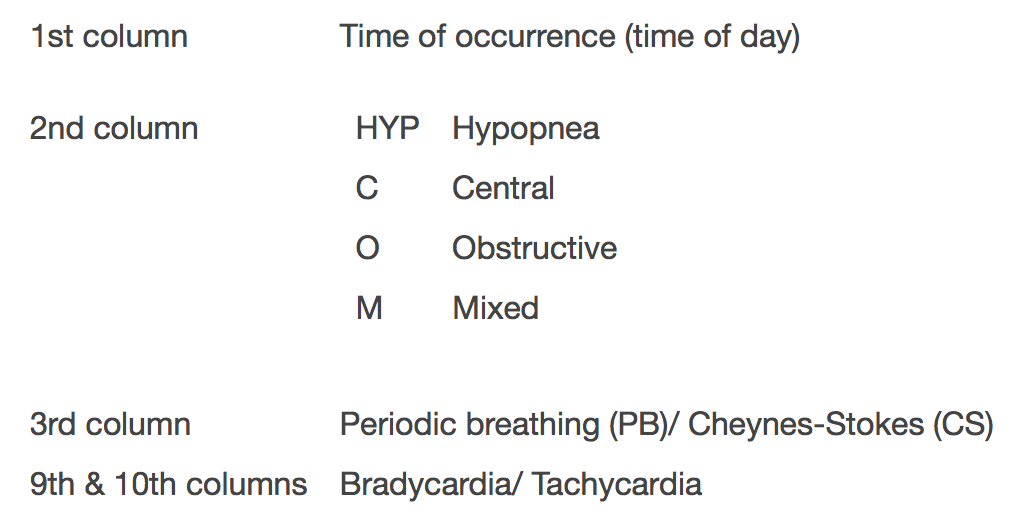
\includegraphics[width=90mm]{Figures/VUH_ANN_respevt.png}}
        \caption{Annotations for St. Vincent's University Hospital database}
        \end{figure}\\
        \textbf{MIT-BIH polysomnographic database: }\\
        Each record in this database has two annotations files, there are .ecg and .st files. The .ecg file contains the beat annotations in wave form while the .st file stores the sleep stage and apnea annotations. Therefore, the .ecg files can be read by following WFDB Programmer's Guide which is made by George B.Moody\cite{MIT_BIH_WFDB}. The .st files contain note-annotations which are sleep staging and apnea information.\\
        \textbf{SHHS polysomnography database: }
        The annotations of this database can be read by using PhysioBank ATM\cite{SHSH_Physiobank} which is free to use from Physionet. The PhysioBank ATM can export the annotations to many different data formats, for example CVS, EDF, Matlab etc. The .hypn contains annotations for sleep stage, the .arou files contains the information on arousal event type and duration, the .oart files contains annotations which present oxygen saturation (SaO2) and their duration, the .resp files contains the annotations for apnea event together with their duration and percent decrease in SaO2, minimum SaO2. The database has also .comp files that are compressed files. The .comp files contains all of the annotations that are stored in the .hypn, .arou, .resp, and .oart files.
    \subsection{EDF and EDF+ formats}
        In recent decades, many efforts to standardize the data format for biosignals have been done. One of them is the European Data Format (EDF). EDF is used for exchanging and storing multichannel biological and physical signals in a simple and flexible way. It was first introduced in 1987 at the Sleep Congress in Copenhagen and then contributed by all participating labs in August 1990\cite{EDF1}. The first publication of EDF was in 1992 in Electroencephalography and Clinical Neurophysiology 82, pages 391-393. The next version of EDF is EDF plus. It was published in 2003 and is compatible to the original EDF version. This is to say all existing EDF viewer programs can use EDF+. On the other hand, EDF+ can contain interrupted recordings as well as annotations, stimuli, and events. It has also fixed some problems that existed in EDF such as Y2K problem, comma vs dot, little-endian integers. Moreover, the EDF+ also supports UTF-8 format. The EDF+ is used in polysomnography, EEG, ECG, EMG and sleep scoring applications. Last but not least, EDF and EDF+ are free to use, and the users and developers can get supports from the EDF site via free downloads of files and software.
        \begin{figure}[ht]
            \centering
            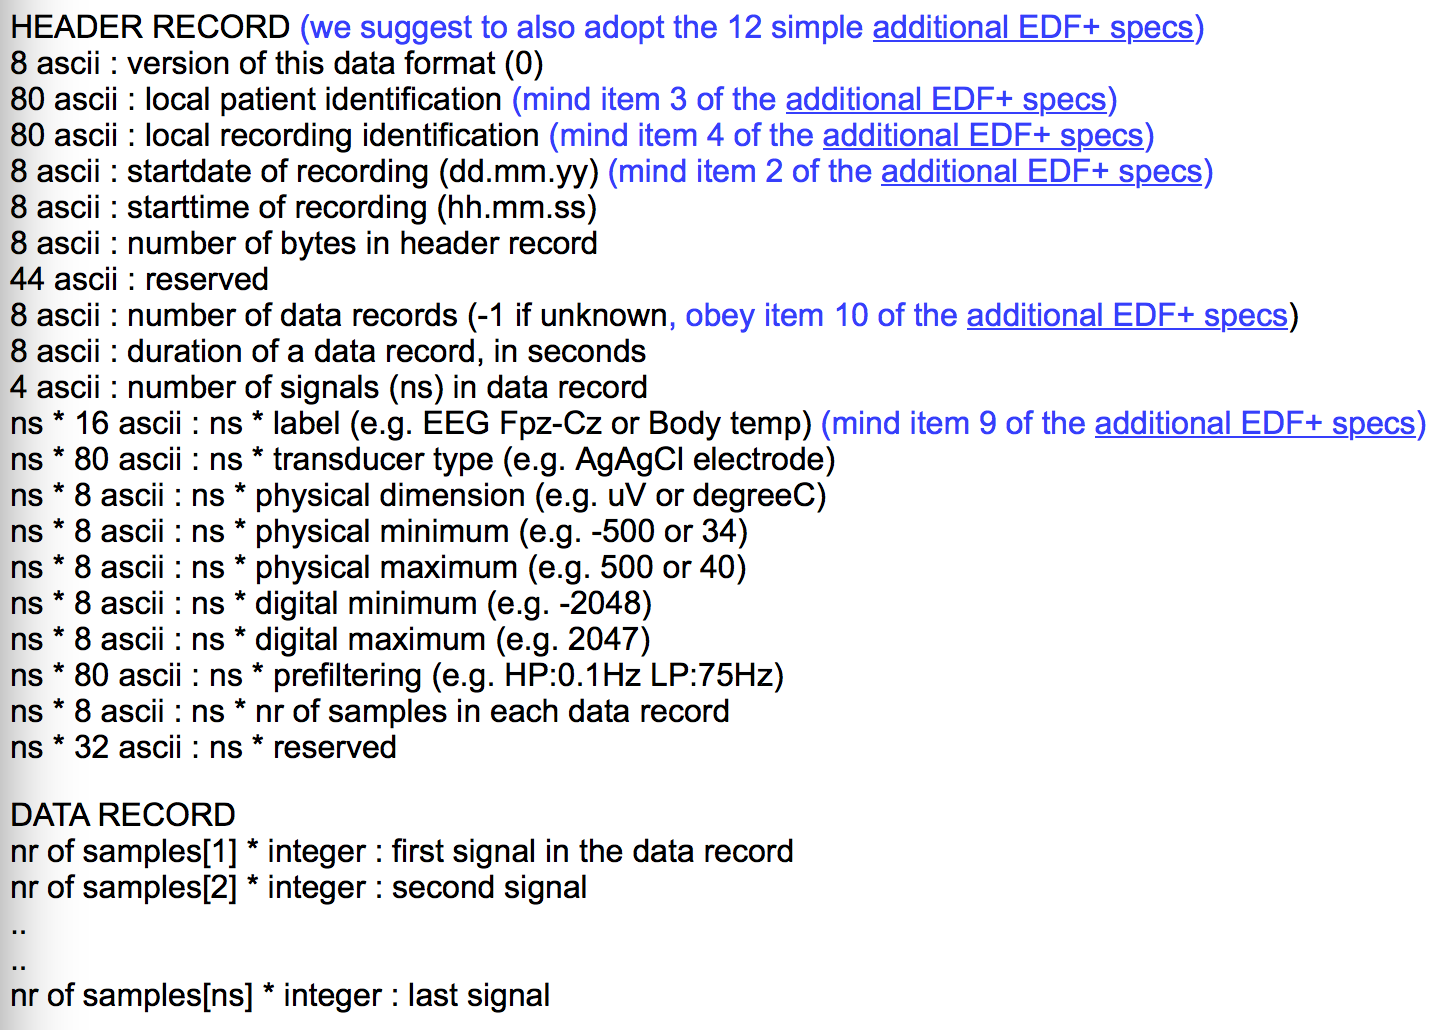
\includegraphics[width=1.0\textwidth]{Figures/EDFFILE.png}
            \caption{EDF and EDF+ file structure \cite{EDF2}}
            \label{fig:edf}
        \end{figure}\\
        Both EDF and EDF+ have the same structure of a data file. As Figure 3.5 presents, the data file consists of two parts which are the header record and the data records. The first 256 bytes of the header part contains the basic information for the record which are the version of the data format (8 ascii), the identifications of the local patient and the local recording (80+80 ascii), start date formated as dd.mm.yy (8 ascii), start time formated as hh.mm.ss (8 ascii), the size of the header record (8 ascii), reserved field (44 ascii), the number of data records followed by the header record (8 ascii), duration of a data record (8 ascii), and the number of signals in data record (4 ascii). The rest of the header record (after the first 256 bytes) contains the information for each field of the signals. Each signal has a label which is not longer than 16 bytes, and coded in ascii. After the label is the transducer type which has the length up to 80 bytes. After the transducer type field is the physical dimension with its maximum and minimum observable values (both physical and digital), each of them is coded in 8 ascii bytes. The following 80 bytes are used to store filters which were used for the signal. The next 8 bytes are used for the number of samples in each data record. The last 32 bytes are reserved.\\
        The data record part consists of a list of data records. Each data record has a list of samples for each signal. For each signal in the record, a sample for the signal is an integer. Hence, the number of bytes for each signal is the number of sample multiply with the size of integer.\\
        The differences between EDF and EDF+ are the information in the 44 bytes reserved field and additional specifications are added to EDF+. In the reserved field, when a record is EDF+ and continuous, it must start with EDF+C, and EDF+D if it is discrete. There are 12 additional specifications in EDF+ which are some rules for the header, date-time, local patient and local recording identification, digital maximum and minimum, separator for digital grouping, endian format, standard texts and polarity rules etc.\cite{EDFpluss}.\\
        The EDF+ data files are coded in a way that they can store both annotations and events. The EDF software can read EDF+ annotations as the physical sensor signals. Because the annotations are treated as signal, the results that are presented in the EDF viewers are strange.\\
        Beside containing ordinary signals, EDF+ can contain annotations signals. The annotations signal is defined by giving it the label "EDF Annotations". Then instead of storing ordinary signal samples, this field can be used for storing notation. This EDF annotations signal can be used for coding the text, time-keeping, events and stimuli as text. The annotations are kept in lists that are named Time-stamped Annotations Lists (TALs).
        \begin{figure}[ht]
            \centering
            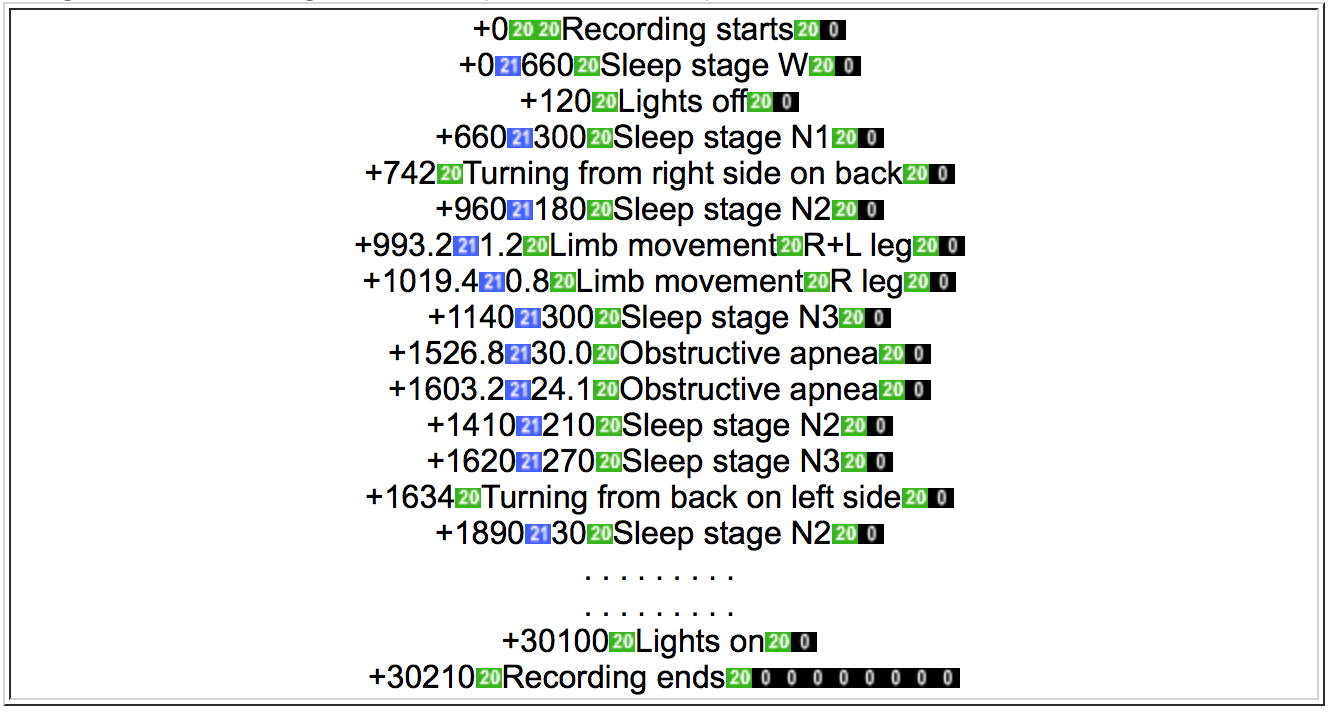
\includegraphics[width=1.0\textwidth]{Figures/Scoringsample.png}
            \caption{Sleep scoring sample\cite{EDFpluss}}
            \label{fig:Figures/Scoringsample}
        \end{figure}\\
        Figure 3.6 presents a sample of TALs for sleep scoring. The annotation signal is defined by giving it the label "EDF Annotations" in the label field in the header part. Then instead of storing ordinary signal samples, this field can be used for storing notation. This EDF annotations signal can be used for coding the text, time-keeping, events and stimuli as text. As presented in Figure 3.6, the annotations for sleep scoring are stored in TALs. Each TAL is formated in form +/-Onset21Duration20Annotation20Annotation20... Annotation20\textbf{0}, where 20, 21 and \textbf{0} are character codes. The Onset presents the amount of time before or after the starting time followed by a value 21 which is unprintable ASCII characters for ending the Onset. After the value 21 is the duration of this annotation. Both Onset and Duration can contains a dot character(float number) to make a better accuracy measurement. After the duration, each annotation can be separated by the unprintable ASCII character 20. The last annotation is followed by unprintable ASCII character 0 for terminating the list.\\
        In EDF+, the data records do not need to be contiguous. Therefore, the start time of each record must be specific. Although the first annotation of the first EDF annotations signal is empty, the timestamp of the annotation must be specified how many seconds after the recording started in term of date and time. Hence, the first TAL in the first data record must start with +0.X\textit{20}\textit{20}, X can be dropped if it is 0.
\section{CESAR data acquisition tools}
    First and foremost the sensor data which are generated by sensors need to be stored. Metadata needs to be defined such that the data can be easily sent, stored, and processed. This section presents two different tools that are used to obtain and store biosignals from different sensor sources (developed by Gjøby\cite{SP}), and from BITalino kit (developed by Carlos Carreiras et.al \cite{StorageBIT}).\\\\
    CESAR is a project that is under developed by a group of universities (University of Oslo, National University of Singapore and Oslo University Hospital). In the Master Thesis by Gjøby\cite{SP}, a generic data acquisition tool for mobile platforms (the Android platform) is presented. This tool is designed such that it is independent from data management and data analysis, and new data sources are also supported by it. An other tool which can be used to obtain biosignals for CESAR is StorageBIT. This tool was developed by Carlos Carreiras et.al \cite{StorageBIT}. StorageBIT is not only a data acquisition tool, but also a database model used for storing biosignals in an efficient way. Regarding the scope of this section, only data acquisition part of StorageBIT is presented in the section.
    \subsection{Generic Data Acquisition for Mobile Platforms}
    Gjøby finished his master degree with the project title "Generic Data Acquisition for Mobile Platforms" at the Department of Informatics at the University of Oslo in spring 2016. He worked on designing and developing an extensible system which allows applications to collect external and built-in sensor data through one common interface. He chose to design and implement a system for Android platform in his master thesis. He presents the overview of the system in the chapter "Not Android Specific". In this chapter, he explains how to design sensor wrappers and providers. A sensor wrapper establishes a connection to a specific data source in order to collect data, after that it sends the collected data to the provider application. Hence, the sensor wrapper needs to be designed to fit the technology of the link layer and communication protocol of the specific data source. Therefore, each data source has its own sensor wrapper. A provider is an extended sensor wrapper management which can use any of the available sensor wrappers. Figure 3.7 illustrates an overview of how sensor wrappers connect to a provider, and a way provider serves multiple applications.
    \begin{figure}[ht]
        \centering
        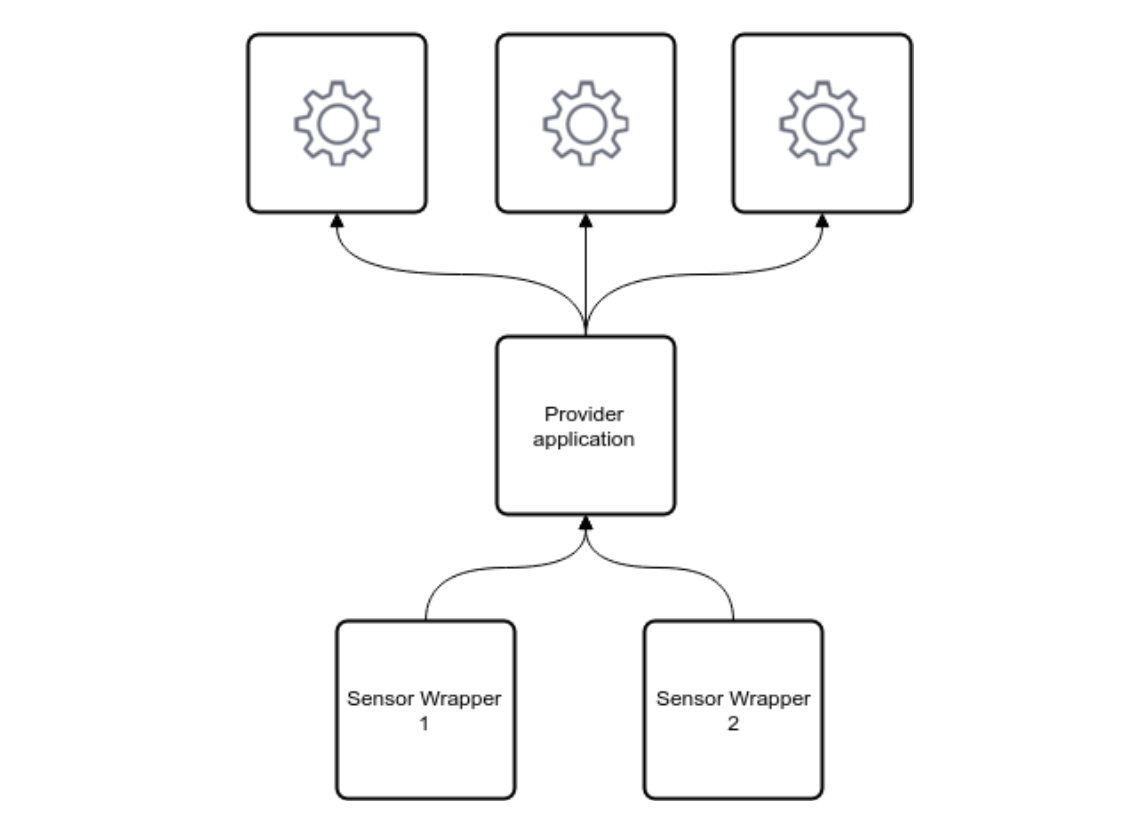
\includegraphics[width=0.5\textwidth]{Figures/provider_SW.png}
        \caption{Sharing the collected data between multiple applications\cite{SP}}
        \label{fig:provider_SW}
    \end{figure}\\
    In the chapter "Android Specific", he implements this design on the Android platform after discussing on the suitable components and functions that Android provides. To collect data from physical sensors and send the collected data to a user application, he defines two JSON structures as illustrates in the Figure 3.8. 
    \begin{figure}[ht]
        \centering     %%% not \center
        \subfigure[A JSON structure describing the encoding of the metadata]{\label{fig:stage}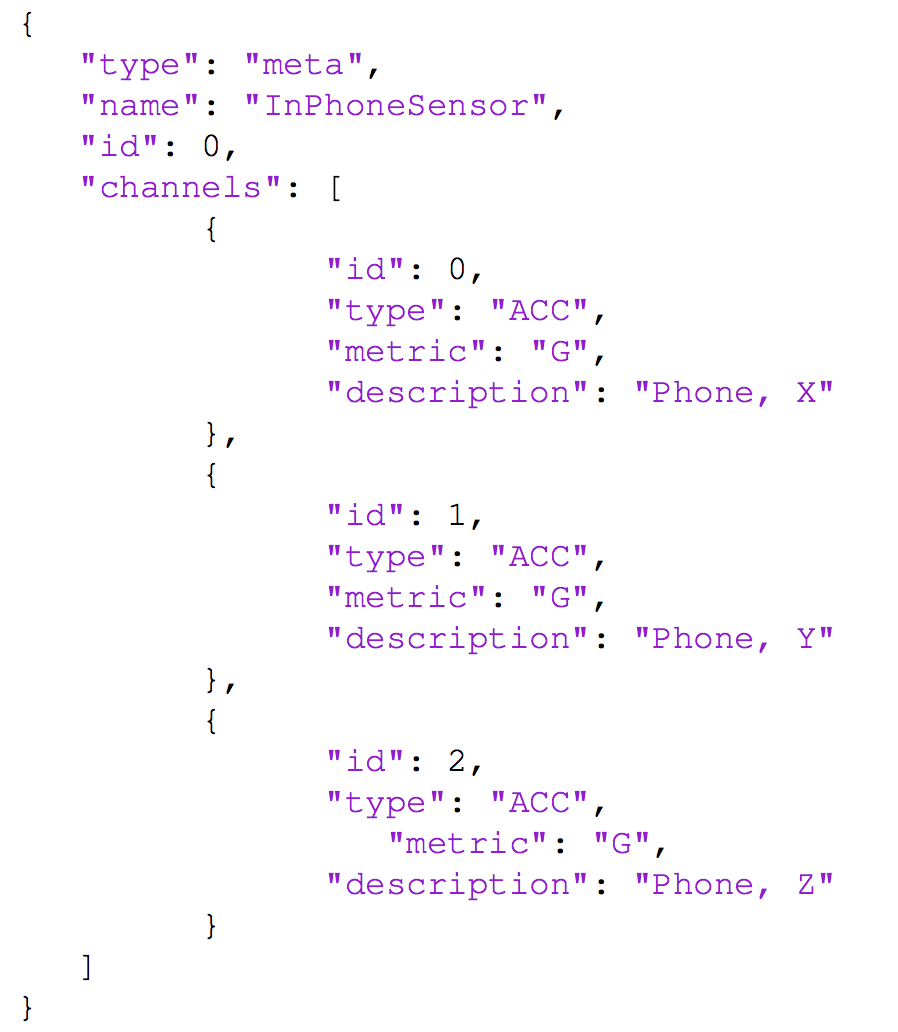
\includegraphics[width=70mm]{Figures/JSONmeta.png}}
        \subfigure[A JSON structure describing the encoding of a data reading]{\label{fig:respevt}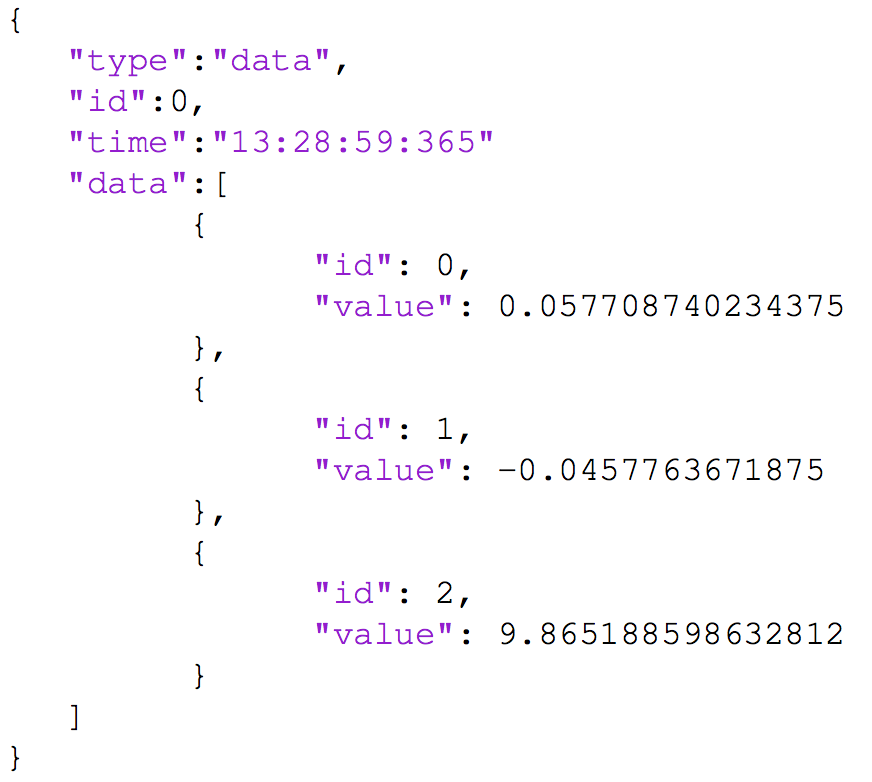
\includegraphics[width=75mm]{Figures/JSONdata.png}}
        \caption{A JSON structures used to send and receive sensor data.\cite{SP}}
        \end{figure}\\
    His application immediately sends a metadata to the application when it receives a connection demand. He defines the metadata in form of a JSON-Object which has as the first element a tuple("type","data"). The second and third elements are name and ID of the sensor wrapper, the remaining elements are the data from the channels, which belong to the sensor wrapper, in form of a JSON-Object array. Each channel has a unique id, type (ACC,ECG,EMG, etc.), metric and description. The JSON-Object is converted to a string and sent to the application. After connected to the BITalino board, the application retrieves data from physical sensors and submits to the application. The connection to the BITalino board should be stopped after receiving a stop signal from the application.\\
    As Gjøby presents in chapter "Not Android specific", the context of the data acquisition is specified as metadata for that it can be used for one common interface. After a comparison between JSON, XML and binary buffer, he decided to use JSON for streaming sensor data in his tool. At first, a metadata which contains general, unchanged information under acquisition (also known as a described context of the collected data from sensor wrapper) is sent, then the collected data from sensors are sent as soon as they are available to avoid overhead. The tool provides a common interface by combining the sensor wrapper ID and the channel ID as abstract level to identify each channel in the system. Figure 3.9 presents a sample of the metadata for BITalino by using a JSON structure. An existing sensor database can be treated as a sensor wrapper with a unique ID. The requested data for a channel in the sensor database can be obtained by using the database ID together with the ID of the requested channel. In other words, the metadata in form of JSON structure for all sensor sources are the same such that they can be used by a provider via one common interface.
    \begin{figure}[ht]
        \centering
        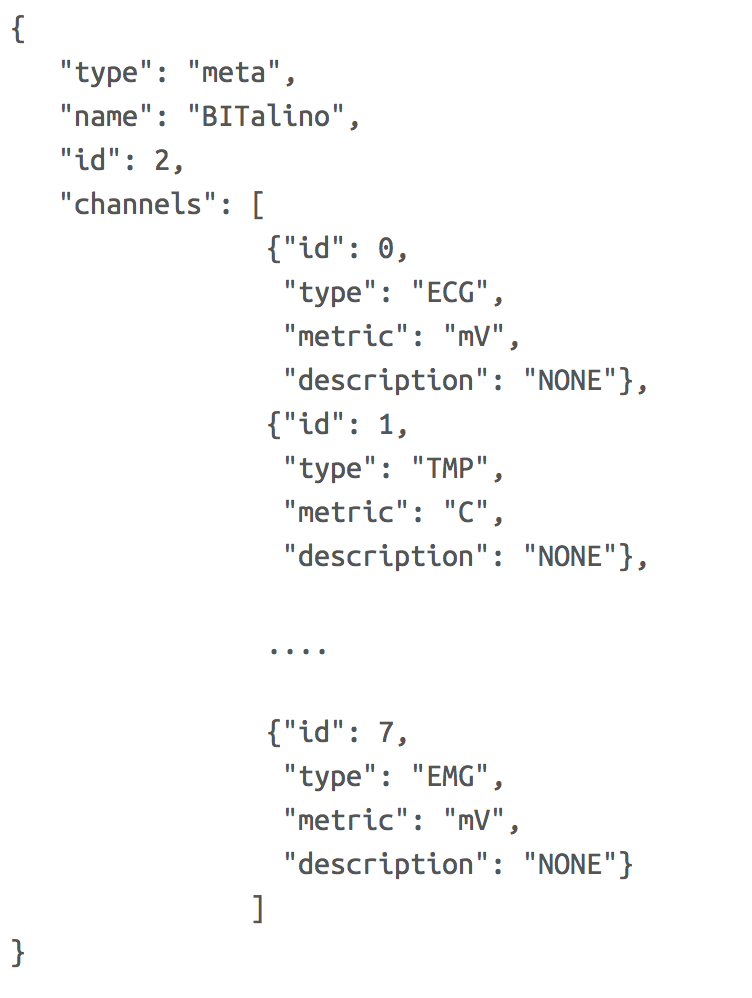
\includegraphics[width=0.5\textwidth]{Figures/metadata.png}
        \caption{A JSON structure sample of the metadata from BITalino}
        \label{fig:JsonGen}
    \end{figure}\\
    Each data sample contains type, sensor wrapper id, timestamp, and the data for the channels. The type of the sample must be "data" such that it can be distinguished with the metadata package which has the type "meta".\\
    Another important component in this tool is a provider. The provider can be considered as a bridge to connect the sensor wrappers with the applications. The provider works as a sensor wrapper management and data processing. It discovers sensor wrappers dynamically by broadcasting a discovery message, then it registers the responded sensor wrappers for later harvesting data. The collected data from sensor wrappers are pushed to the provider by using earlier mentioned JSON structure. Then, the provider processes the data, i.e, stores or forwards the data to an application.
    \subsection{StorageBIT data acquisition}
    Carlos Carreiras et.al \cite{StorageBIT} have done research on storing biosignals from BITalino. This tool can convert sensor data from different sources into their data model. Although the tool mainly supports the BITalino kit, it can also manage other sources by mirroring these sources into its data model. At first they make a comparison of the existing data formats which are the Extensible Biosignal File Format (EBS), the European Data Format (EDF and EDF+), the Medical Waveform Format Encoding Rules (MFER) and the Waveform Database(WFDB) based on eight properties which are compression, non-sequential access, cross platform support, events support, extensibility, metadata, multi modality and querying. After that, they make a data model which has "Records" as the basic abstract entities for storage. Each record consists of header, audit, biosignals and events and is stored in form of JSON-Object as presented in Figure 3.10. 
    \begin{figure}[ht]
        \centering
        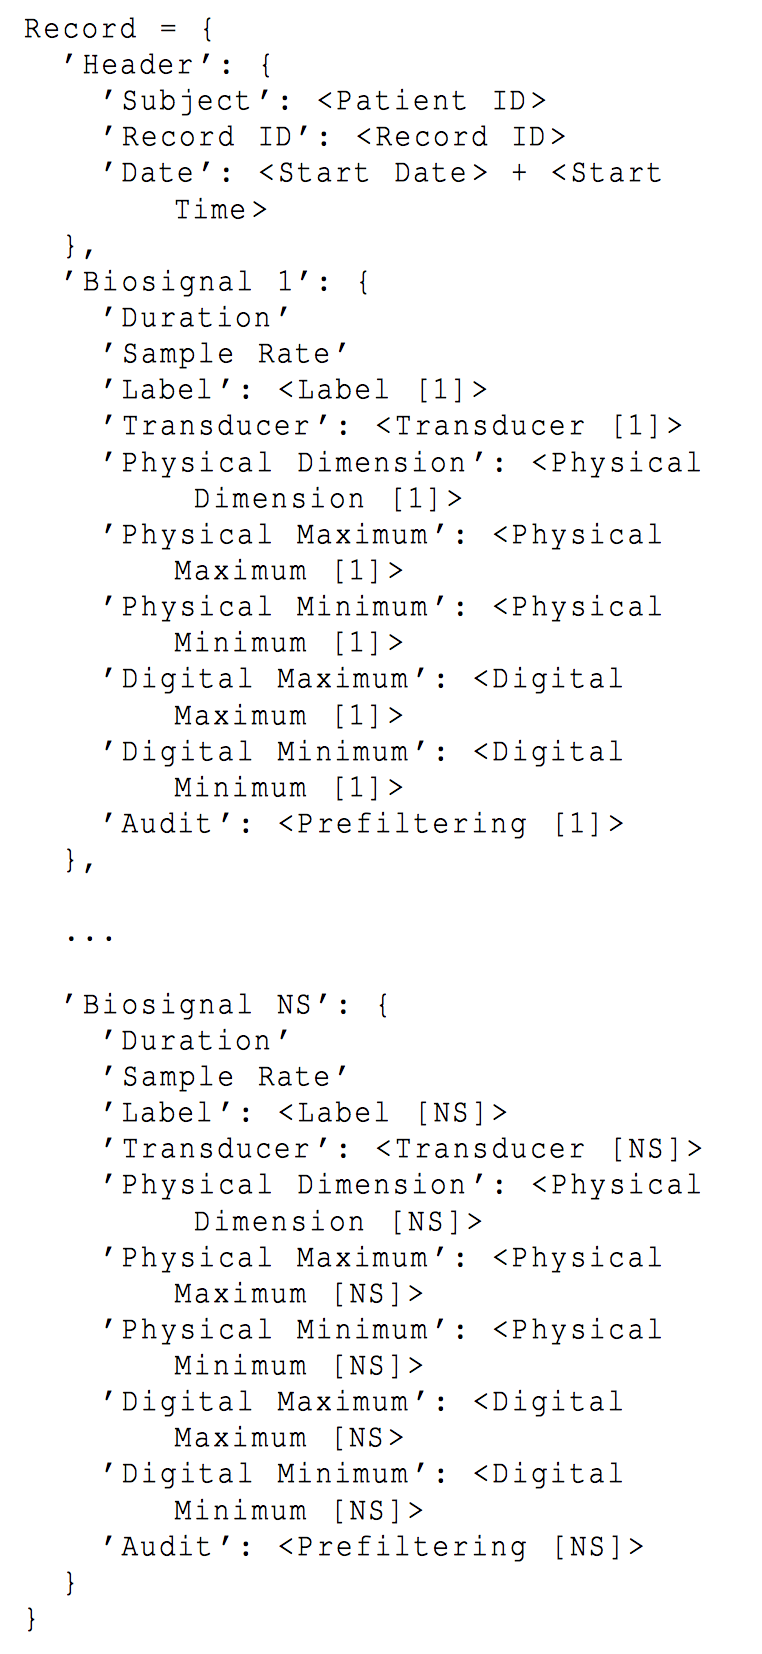
\includegraphics[width=0.5\textwidth]{Figures/metadata2.png}
        \caption{Mirroring of the EDF+ file structure onto the Data Model \cite{StorageBIT}}
        \label{fig:JsonStorageBIT}
    \end{figure}\\
    The header contains the basic information such as the patient identification, when and where the record was taken, and who performed the acquisition. The audit field contains the history of the file such as the applied filters or processing steps etc. The biosignal filed contains the data of the interested signals such as observing duration, sample rate, the label of the signal, transducer etc. The events field contains any asynchronized information like annotations or any events which are not synchronously from time series.
\lhead{\emph{Database modeling}}
\chapter{Database modeling}
It is well recognized that the design of a database has a huge influence on the quality of the database applications. To design a database means to build a formal model for the database application. The data model does not only define a logical structure of a database, but also determines a set of rules and operations which could be used for performing actions on the data. All of data items that have meaning in the real world can be stored in a file system. A file is a collection of the data items, and need to be managed in a way that can be easily read and updated. A relational database is one of the ways that are used for managing files. In the relational database, a smallest unit of data in the real world can be mapped into an attribute that belong to a certain entity in a database. In term of database’ components, the smallest unit of data is called a column, a group of related columns is called a tuple or a row. Each row reflects to a specific object in real world, and these rows are abstracted into a table. In order word, the table presents an entity type in the database system.\\
To make the analyzing OSA data easier, a database system is taken into considering. The mentioned data sources in Chapter 3 using files to store their bio-signal data. As a result, they do not take advantages of using offered functions of a database management system for doing data analyzing. On the other hands, each source can be used by a single user at the time, and therefore, to do comparing the quality of sources is very difficult. Hence, the needs of storing the OSA data into tables in a database system must be seriously considered.
This chapter presents a data model for storing OSA bio-signal by analyzing requirements of users and data sources. Based on the requirements, a data modeling procedure is performed to find the most suitable database model for storing OSA data.\\
Section 4.1 presents requirements for the OSA database, in which the requirements are grouped into group of users, and the requirements of the sensor sources. Section 4.2 presents conceptual data modeling. In this section, entities and their relationships are defined. From that, a logical model is derived as presented in Section 4.3. The logical model is independent from a database management system. It only presents the structure of the database, therefore database conversion and reorganization are much easier to be taken. In section 4.4, a specific database management is chosen to implement the logical database model. Since an Android mobile platform is used to collect OSA samples (CESAR acquisition tool), and the thesis would like to build a database application for CESAR on mobile platform, SQLite database management system is chosen to implement the database model.
\section{OSA database system requirements}
When designing a database, it is essential to identify requirements. The requirement for a database system usually focus on two things, that are what the database is to be used for, and what it must contain. In term of storing OSA data, the data system must satisfy requirements of the sensor sources (what it must contain), and requirements of users who using it (what the database is to be used for). There are three main groups of user, which are patients, physicians and researchers. These users would like to have a database system to keep track of collected bio-signals from both CESAR acquisition tool (BITalino sources) and other sources in form of EDF format (Physionet databases). The database system must support the future changes in OSA such that the system does not need to be rewritten.\\
Since the source data for the database system are the CESAR acquisition tool and the EDF/EDF+ file format, the system must at least store all of data items from them. The data items of the CESAR acquisition tool and the EDF/EDF+ file format are presented in Table \ref{tab:Datasources}, where derived data items in EDF format such as number of bytes in header, number of data records, etc., are not included in the table. Description column presents the interested objects, and these objects must be stored in the database system.
\begin{table}[ht]
\begin{center}
\begin{tabular}{ |p{3.3cm}||p{5cm}|p{5cm}|  }
 \hline
 Description& CESAR acquisition tool & EDF/EDF+ file format \\
 \hline
 The identifier of a source& Wrapper id& n/a\\
 \hline
 Name of source& Wrapper name& File name\\
 \hline
 The identifier of a channel& Channel ID& n/a\\
 \hline
 Name of channel& Data type& 16 ascii: signal label\\
 \hline
 Metric& Metric& 8 ascii: physical dimension\\
 \hline
 Recording description& Description& 44 ascii: reserved field\\
 \hline
 Information of patient& n/a& 80 ascii: local patient identification\\
 \hline
 Information of clinic& n/a& 80 ascii: local recording identification\\
 \hline
 Recording fragment& n/a& Data record\\
 \hline
 Fragment duration& n/a& 8 ascii: duration of a data record, in second\\
 \hline
 Number of used channels& Can derived from metadata package& 4 ascii: number of signals in data record\\
 \hline
 Transducer type& Can derived from BITalino documents& 80 ascii: transducer type\\
 \hline
 Physical maximum& Can derived from BITalino documents& 8 ascii: physical maximum\\
 \hline
 Physical minimum& Can derived from BITalino documents& 8 ascii: physical minimum\\
 \hline
 Digital maximum& n/a& 8 ascii: digital maximum\\
 \hline
 Digital minimum& n/a& 8 ascii: digital minimum\\
 \hline
 Pre-filtering& n/a& 80 ascii: prefiltering\\
 \hline
 Number of samples in a fragment& n/a& 8 ascii: number of samples in each data record\\
 \hline
 Other information for a channel& n/a& 32 ascii: reserved\\
 \hline
 Timestamp for a sample& Can derived from data package& Can calculate from timestamp of the recording\\
 \hline
 Sample value& Float type value& 2-byte integer, a guide to convert between these bytes to float and vice versa\\
 \hline
\end{tabular}
\end{center}
\caption{A summary of data items from CESAR acquisition and EDF/EDF+ file format}
\label{tab:Datasources}
\end{table}
In term of what the database is to be used for, the user requirements need to be considered such that the database can be designed in a way it satisfies the requirements of the users. The requirements can be derived from activities the users perform on data in the system. 
\begin{table}[ht]
\begin{center}
\begin{tabular}{ |p{3cm}||p{10cm}|}
 \hline
 User group& Action\\
 \hline
 Patient&- Find recordings, physicians, clinics\newline
 - Store samples from CESAR tool\newline
 - Retrieve samples for certain channels\newline
 - Import their previous recording\newline
 - Export certain sources or channels\newline
 - Export part of a recording for some channels\newline
 - Delete a specific source\newline
 - Delete them self from database\newline
 - Import trained OSA data from physician\newline
 - Execute mining to find out OSA for a new recording based on a trained source\\
 \hline
 Physician&- Find patients, recordings, clinics\newline
 - Import EDF file from patient\newline
 - Store samples from CESAR tool\newline
 - Retrieve all recording for a patient\newline
 - Retrieve samples for a channel from different patients to do comparison\newline
 - Retrieve part of recordings for some channels\newline
 - Update annotations for a recording\newline
 - Export recoding to EDF file to share with other physician or researcher\newline
 - Delete a source, a recording, a patient, etc.\newline
 - Manual training data for a recording by taking annotations while visualizing sources\newline
 - Execute mining algorithm to find AHI for new sources\\
 \hline
 Researcher&Beside the basic actions as the patients and physician have, researchers can perform more advance actions such as:\newline
 - Evaluate the quality of sources and channels that are used for collecting sample\newline
 - Perform raw query to find out the best query algorithms, which cost minimum resources when executed, minimum running time\newline
 - Apply possible mining algorithms to find out the best fixed for the database model which implemented in a specific database management system\newline
 - Evaluate the possibility of database system when implemented on different hardware mobile platform\newline
 - Develop an interested database application base on the database model\\
 \hline
\end{tabular}
\end{center}
\caption{A summary of user requirements}
\label{tab:userrequirementDB}
\end{table}
Table \ref{tab:userrequirementDB} presents a list of possible actions the patients, physicians, and researchers interact with the database system.\\
To make it is easy to follow, a brief for the actions that are presented in Table \ref{tab:userrequirementDB} is taken into discussion. The mains activities of the patents on the database system are functions that do inserting, simple querying and deleting. Therefore, most of their actions are import and export. Some of functions (pre-define queries) can be defined for the patients. Hence, the patients are not allowed to use modifying functions, or self-defined functions. The physician, on the other hands, can execute modifying functions, because they are allowed to manually train the data. In other word, the physicians have knowledge on OSA health problems, and they know which signals are abnormal. Therefore, the system must support modifying functions such that the physicians can quickly update the abnormal signals. In contrast, the main focuses of the researchers neither inserting nor updating functions (they also use them, but they are not the main focuses). The researchers often perform evaluating tasks on the system to find the best solutions for future use. In term of OSA database system, they would like to evaluate the quality of sources that are used for collecting bio-signals. Underestimated sources must not be further considered, since they provide inaccuracy data, which lead to many problems when performing data analysis. They researchers can also evaluate different algorithms with respect to resources used, performance, etc. on the database system, since an algorithm can be good for a specific system, but behave badly on the other systems. An algorithm should not be chosen randomly; it must be evaluated carefully. Nevertheless, the database design must can be used by different database applications on different operative system platforms.
\section{Conceptual data modeling}
“Conceptual modeling is about describing the semantics of software applications at a high level of abstraction”\cite{CONCEPTUAL_BOOK}. Similarly, conceptual data modeling can be understood as the semantics of database at a high level of abstraction. Therefore, this section describes only entity names and their relationships. Attributes and keys are not included in the section to maximize the abstraction. As described in Section 4.1, and as presented in Table \ref{tab:Datasources} and \ref{tab:userrequirementDB}, data items that the database system must keep track of are source identifier, source name, channel identifier, channel name, metric, recording description, patient, clinic, recording, recording timestamp, recording fragment, recording fragment duration, transducer type, physical maximum, physical minimum, pre-filtering, number sample in a fragment, reserved information for a channel, sample timestamp, sample of recording, physician who works for clinic, annotation, patient name, patient gender, patient date of birth, patient code in clinic (patient information from EDF), clinic code, physician code, and used equipment by clinic (clinic information from EDF). However, not all of the data items are considered as entities of the database system. As Toby et.al\cite{DATABASEMODELING_BOOK} presents in their Database Modeling and Design book, an entity should contain descriptive information while an attribute is not. An attribute is a data element which requires only one identifier, in addition, attribute does not have any relationships. In addition, multivalued attributes are classified as entities, and attributes must be attached to the closest entities they describe. The Patient entity and Physician entity have a lot of common attributes, it is to say, they are Person. Therefore, a new entity, which is Person, must be defined such that the Patient and Physical can extend from this new entity. As a result, Person is added to the set of entity of the database system.\\
\begin{table}[ht]
\begin{center}
\begin{tabular}{ |p{3cm}||p{10cm}|}
 \hline
 Entity& Attribute\\
 \hline
 Source& source identifier, source name, channel number, channel name, metric, transducer type, physical maximum, physical minimum, digital maximum, digital minimum, EDF reserved compatible\\
 \hline
 Recording& recording id, source identifier, channel number, id person collects recording, id person own recording, recording timestamp, recording description, recording fragment index, recording fragment duration, frequency, pre-filtering, fragment timestamp, sample timestamp, sample value as text (for annotation), sample value as floating point number, used equipment, EDF reserved for recording\\
 \hline
 Person& person id, name, city, phone number, email, gender, data of birth, age, height, weight, BMI, patient id, physician id, other health issues, title in clinic\\
 \hline
 Clinic& clinic code, name, address, phone number, email\\
 \hline
\end{tabular}
\end{center}
\caption{Classified entities with their attributes}
\label{tab:entitiesAttributes}
\end{table}
Based on their guidelines, the data items can be classified into entities and attributes as presented in Table \ref{tab:entitiesAttributes}.In terms of future analysis, some attributes are added to the entities as meta-data for later analysis such as fragment index, source type, fragment timestamp, fragment duration, recording at a frequency, sample value as annotation, sample timestamp, etc. Figure \ref{fig:Figures/RecordingExample} presents how these attributes are used in terms of future analysis.
\begin{figure}[ht]
    \centering
    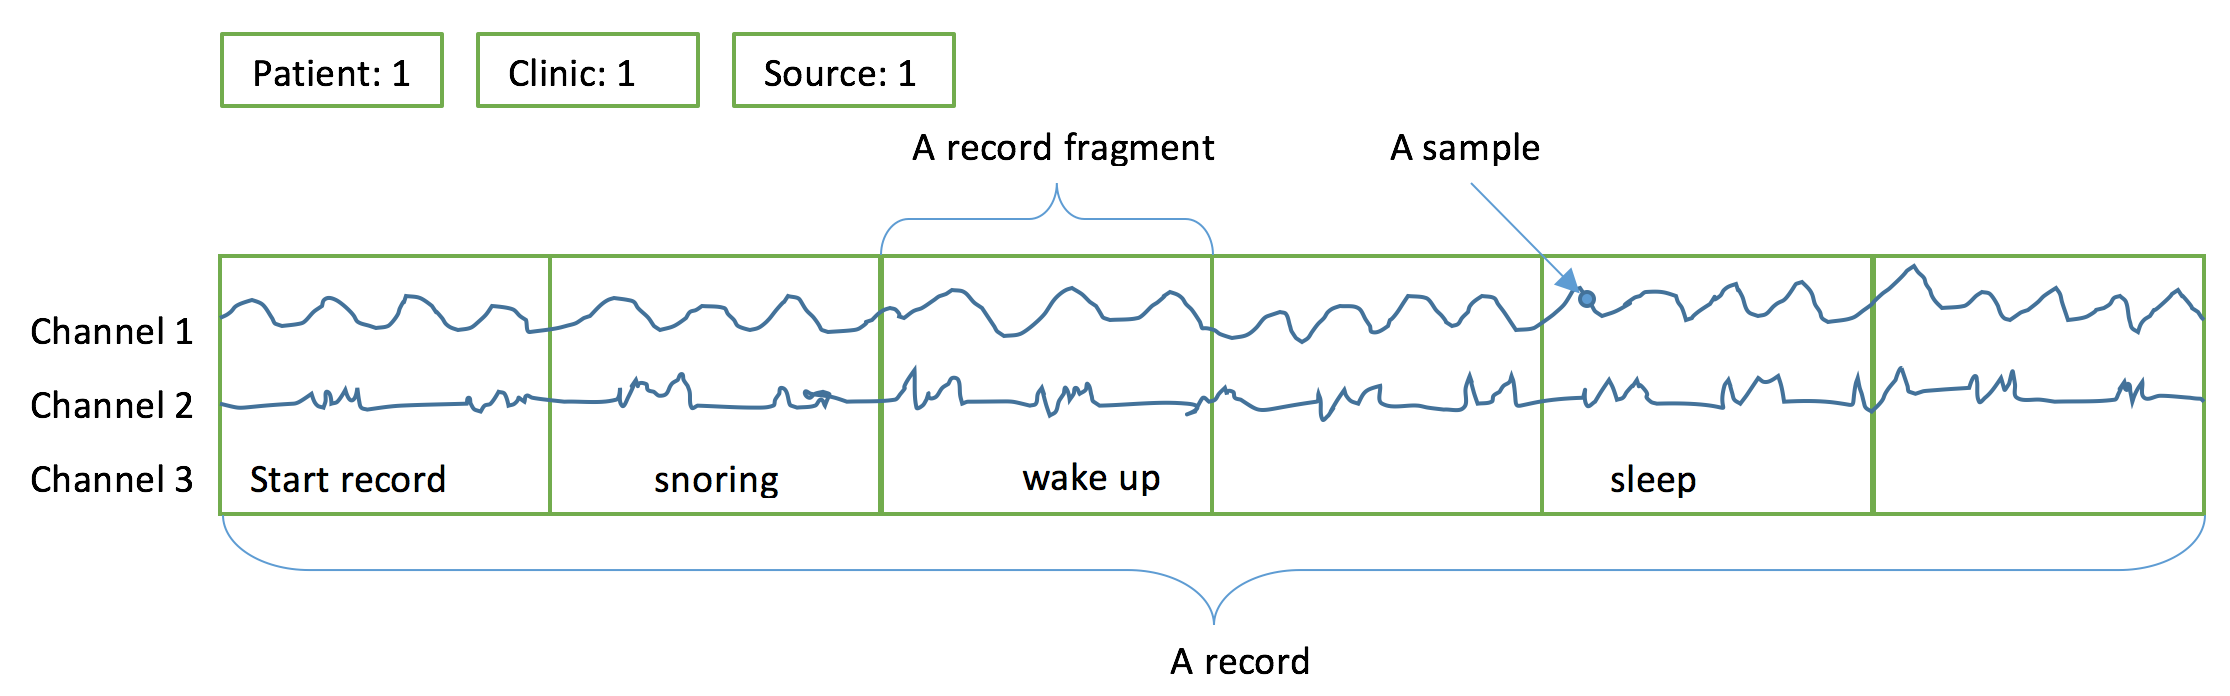
\includegraphics[width=1.0\textwidth]{Figures/ARecord.png}
    \caption{Example of a recording from a source}
    \label{fig:Figures/RecordingExample}
\end{figure}
One of the most important part of the conceptual data modeling is to define relationships between the classified entities. In this part, the Object Role Modeling (ORM) is used for presenting the relationships between entities. ORM is chosen because it is a method for designing and querying database models at the conceptual level, and easy to validate and evolve\cite{ORMdotNET}.\\
A short history of ORM, the term “object-role model” was mentioned in Eckhard Falkenberg’s doctoral thesis which was published in 1976\cite{Wiki_ORM}. ORM is a very good method which is used for designing and querying database models at the conceptual level. ORM uses natural language, as well as diagrams to simplify the design process. With ORM, a conceptual approach to modeling is provided by expressing the model in terms of natural concepts, such as objects and roles. Elementary facts are fundamental for ORM. These elementary facts are expressed in diagrams, and are verbalized into natural language. Nevertheless, modeling, transforming, and querying data from a domain become much easier with the help of the “fact-based” approach. ORM is easily to understand by non-technical users, because it is attribute free. It is to say, all the facts are treated as relationships. Moreover, when drawing a graphic, it is more expressive and easier to be understood by people without technical background. Last but not least, avoiding attributes in the database model does not only improve the semantic stability, but also enables the verbalization into natural language.\\
Based on classified entities, facts of the database system can be expressed as below:
\begin{adjustwidth}{1cm}{}
•	Source has Recording for Patient(Person) at Clinic.\\
•	Recording for Patient(Person) is produced by Physician/Patient(Person) by using Source.\\
•	Patient/Physician(Person) at Clinic uses Source to produce Recording.\\
•	Physician(Person) work for Clinic.\\
•	Patient(Person) belongs to Clinic.
\end{adjustwidth}
There is another view of the conceptual data model where entity Recording is treated as a relationship. Facts that respected to this view are as below:
\begin{adjustwidth}{1cm}{}
•	Source uses by Patient(Person) at Clinic.\\
•	Patient(Person) at Clinic uses Source.\\
•	Physician(Person) uses Source for Patient(Person).\\
•	Physician(Person) work for Clinic.\\
•	Patient(Person) belongs to Clinic.
\end{adjustwidth}
The second view is easy to read. However, when transform this view into logical model, a product from “uses” must be defined, and it is a Recording with respect to the first view. It is to say, there are a lot of possible views when doing conceptual data modeling. It is difficult to say which is the best view to use. Therefore, these views need to be integrated. Toby et.al[cite] also suggest four steps for conceptual schema integration, they are pre-integration analysis, comparison of schema, conformation of schema, merging and restructuring of schema. Integration for the views in this part is simple. The first view is extended from the second view, hence, it has a better presentation compared with the second view.\\
Figure \ref{fig:Figures/ConceptDB1} presents the first view where Recording is presented as an entity, while in Figure \ref{fig:Figures/ConceptDB2}, Recording is presented as a relationship. As argued in view integration, Figure 1 illustrates the conceptual model of the database system. The notations, that are used in Figure \ref{fig:Figures/ConceptDB1} and \ref{fig:Figures/ConceptDB2}, can be found in the ORM article written by Terry Halpin\cite{ORMdotNET2}
\begin{figure}[ht]
    \centering
    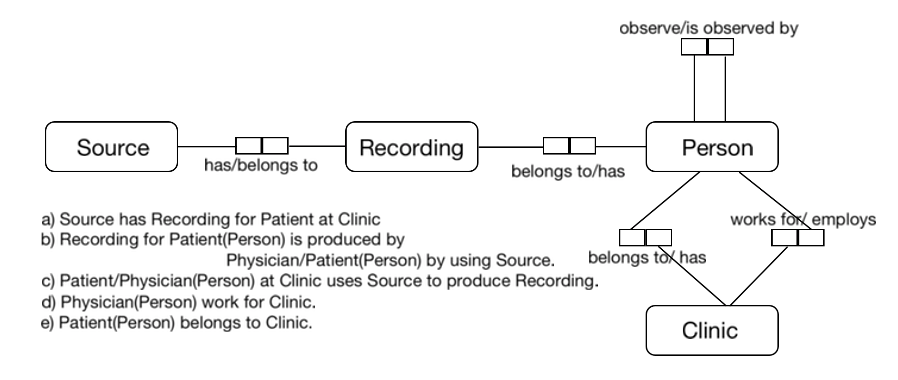
\includegraphics[width=1.0\textwidth]{Figures/ConceptDB1.png}
    \caption{View where Recording is presented as an entity}
    \label{fig:Figures/ConceptDB1}
\end{figure}
\begin{figure}[ht]
    \centering
    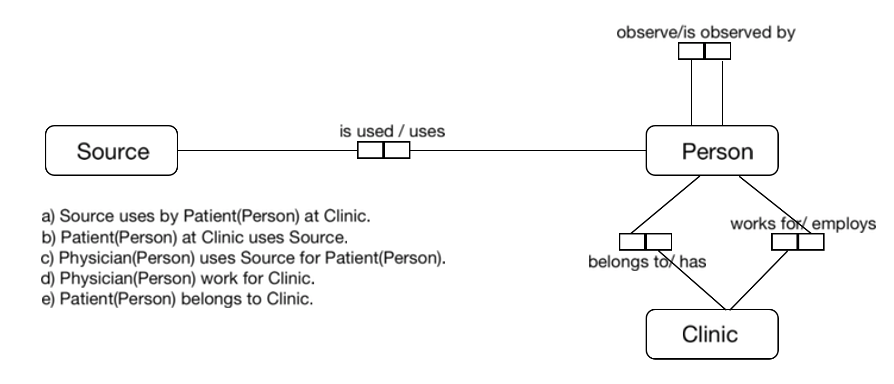
\includegraphics[width=1.0\textwidth]{Figures/ConceptDB2.png}
    \caption{View where Recording is presented as a relationship}
    \label{fig:Figures/ConceptDB2}
\end{figure}
\section{Logical data modeling}
Logical data model describes the abstract structure of the database system. Therefore, it is independent of a particular database management system. That means it does not describe what data types should be used, which technologies can be used such that queries can execute fast, etc., but it should describe tables (entities) and columns (attributes), relationships, etc., in which the primary keys for columns and the reference keys must be specified. Logical data model also presents relationships between entities. Therefore, all entity relationships need to be specified. Then, all attributes for each entity must be carefully identified. Since this thesis takes the future growth of data and meta-data of OSA database into considering, it is essential for finding all possible attributes for the specified entities that described in Section 2. After that, a set of function dependences (FDs) can be derived from the relationships and attributes. Finally, database normalization need to be performed such that the database can be accurate, fast, and efficient. Subsection 3.1 presents the relationships between classified entities. In this subsection, many-to-many relationships are also resolved. Normalization and step by step to normalize are discussed and presented in Subsection 3.2.
\subsection{Relationships between different entities}
Based on the facts that are presented in Section 2, the data relationships are described as the following assertions:
\begin{adjustwidth}{1cm}{}
•	Each Source has many Recordings, but one Recording belongs to only one Source.\\
•	Each Source can be used by many different Person, and each Person can use many different Sources.\\
•	Each Source can be used by many different Clinics, and each Clinic can use many difference Sources.\\
•	Person has many Recordings, but one Recording belongs to only one Person.\\
•	Person collects many Recording, but one Recording is collected by only one Person.\\
•	Each Recording is produced by a Source, for a Person at a certain Clinic at a certain time.\\
•	Each Person works/belongs to many Clinics, and each Clinic employs/has many Person.\\
•	Each Person (Physician) observers many Persons (Patient), and many Person(Patient) are observed by a Person(Physician).
\end{adjustwidth}
These relationships can be divided into three groups: binary relationships, binary recursive relationships and ternary (or n-ary) relationships. Figure \ref{fig:Figures/RelationshipBinary} and \ref{fig:Figures/NaryAndRecursive} present these relationships by using ORM notations.\\
\begin{figure}[ht]
    \centering
    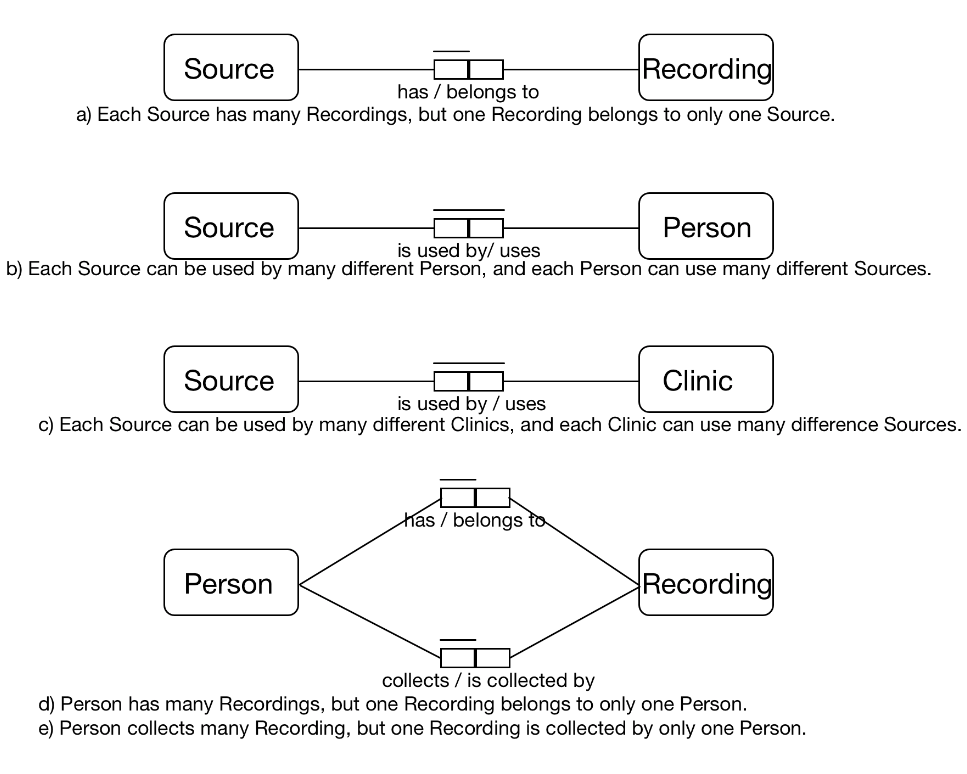
\includegraphics[width=1.0\textwidth]{Figures/RelationshipBinary.png}
    \caption{Binary relationships}
    \label{fig:Figures/RelationshipBinary}
\end{figure}
\begin{figure}[ht]
    \centering
    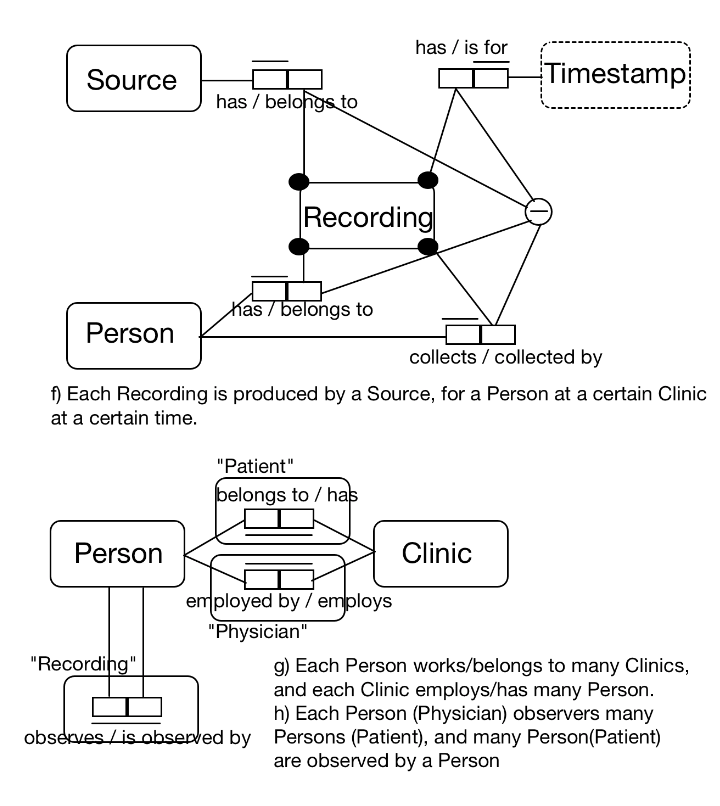
\includegraphics[width=1.0\textwidth]{Figures/NaryAndRecursive.png}
    \caption{Recursive and n-ary relationships}
    \label{fig:Figures/NaryAndRecursive}
\end{figure}
Foreign keys are easily derived from binary relationships. If there is a one-to-one binary relationship, the key of either entity can be used in other entity’s table as a foreign key. If there is a one-to-many binary relationship, the foreign key must appear on the “many” side, since “many” side presents the child entity. A many-to-many binary relationship must be resolved, since the relational database management system cannot hold this relationship. An easiest way to resolve a many-to-many binary relationship is to convert this relationship into a new entity, in which each old entity has a one-to-many binary relationship with the new entity. In the thesis, it is natural to see that most of the many-to-many binary relationships from the assertions can be resolved by using Recording entity as a new entity between the old entities. Physician and Patient can be used as new entities for relationships “works/belongs to” and “employ/has” respectively in the assertion “Each Person works/belongs to many Clinics, and each Clinic employs/has many Person”. As a result, the new entities must contain foreign keys that refer to parent entities.\\
In a binary recursive relationship between two Persons (A Person observes a Person), a foreign key refers to a column which identifies the referred Person. The 4-ary relationship “Each Recording is produced by a Source, for a Person at a certain Clinic at a certain time” presents that Recording is depended on a Source, a Person and a Clinic at a specific time, therefore it must contain the primary keys of these entities as foreign keys.\\
Most of attributes for each entity can be taken from Table \ref{tab:entitiesAttributes}. Table \ref{tab:EntitiesFDs} presents the entities together with their attributes and FDs, and it is a result of the analysis. In this table, each attribute of a entity is given an alias for saving writing when finding primary keys and decomposition. 
\begin{table}[ht]
\begin{center}
\begin{tabular}{ |p{1.5cm}||p{5cm}|p{6.5cm}|  }
 \hline
 Entities& Attributes& Function dependents\\
 \hline
 Source& source identifier (A), source name (B), channel number (C), channel name (D), metric (E), transducer type (F), physical maximum (G), physical minimum (H), digital maximum (I), digital minimum (J), EDF reserved compatible (K), source type (L)& \textbf{A,C} $\rightarrow$ D, E, F, G, H, I, J, K\newline \textbf{A} $\rightarrow$ B, L\\
 \hline
 Recording& recording id (A), source identifier (B), channel number (C), id person collects recording (D), id person own recording (E), recording timestamp (F), recording description (G), recording fragment index (H), recording fragment duration (I), frequency (J), pre-filtering (K), fragment timestamp (L), sample timestamp (M), sample value as text (for annotation) (N), sample value as floating point number (O), used equipment (P), EDF reserved for recording (Q)& \textbf{A} $\rightarrow$ B, D, E, F, G, I, J, K, P, Q\newline \textbf{B,D,E,F} $\rightarrow$ A, G, I, J, K, P, Q\newline \textbf{A,H} $\rightarrow$ L\newline \textbf{A,B,C,H,M} $\rightarrow$ N,O\\
 \hline
 Person& person id (A), name (B), city (C), phone number (D), email (E), gender (F), data of birth (G), age (H), height(I), weight(J), BMI(K), clinic code patient(L), clinic code physician(M), other health issues (N), title in clinic(O)& \textbf{A} $\rightarrow$ B, C, D, E, F, G, H\newline \textbf{A,L} $\rightarrow$ I, J, K, N\newline \textbf{A,M} $\rightarrow$ O\\
 \hline
 Clinic& clinic code (A), name (B), address (C), phone number (D), email (E)& \textbf{A} $\rightarrow$ B, C, D, E\\
 \hline
\end{tabular}
\end{center}
\caption{OSA entities with their attributes and FDs}
\label{tab:EntitiesFDs}
\end{table}
Based on the defined function dependents of the entities, primary keys of these entities can be found by following these steps\cite{INF3100_Recipe_book}:
\begin{adjustwidth}{1cm}{}
With FDs belong to a relation/entity R:\\
1. Let X = a set of attributes that are not exist in any right hand side if the FDs.\\
2. Expand systematic X in every possible ways with the attributes that occur at least one on left hand side of FDs.\\
Compute closure X+ for each such X until X+ are all attributes.\\
If X+ are all attributes in R, check that whatever an attribute A is chosen in X, (X-A)+ is not a set of all attributes of R.\\
If that is the case, X is a candidate (primary) key.
\end{adjustwidth}
A algorithm, that is used for computing a closure of the attribute set with respect to FDs, is as follow\cite{INF3100_Recipe_book}:
\begin{adjustwidth}{1cm}{}
Let X is a set of attributes in relation, and X+ is a closure of X.\\
1. T := X\\
2. As long as T changed, if there is a FD A $\rightarrow$ B in FD set, where A is a subset of T, T:=T$\cup$B\\
3. X+ := T
\end{adjustwidth}
\textbf{Source}\\
A and C are not presented in the right hand side of the two FDs. After computing AC+, all of attributes are retrieved.
Therefore, AC is the only candidate key of this entity\footnote{To be easy to follow, entity, relation, and table are used alternatively.}.\\
\textbf{Recording}\\
A, C, H, and M are not presented in the right hand side of the FDs. After computing ACHM+, all of attribute are retrieved. Therefore, ACHM is the only candidate key of this entity.\\
\textbf{Person}\\
A, L, and M are not presented in the right hand side of the FDs. After computing ALM+, all of attribute are retrieved. Therefore, ALM is the only candidate key of this entity.\\
\textbf{Clinic}\\
All of other attributes depend on A, therefore A is the only candidate key of this entity.\\
Table \ref{tab:entitiesPrimaryKey} presents the results after performed the key-finding algorithms.\\
\begin{table}[ht]
\begin{center}
\begin{tabular}{ |p{3cm}||p{10cm}|}
 \hline
 Entity& Primary key / candidate key\\
 \hline
 Source& (source identifier, channel number) as AC\\
 \hline
 Recording& (recording id, channel number, recording fragment index, sample timestamp) as ACHM\\
 \hline
 Person& (person id, clinic code patient, clinic code physician) as ALM\\
 \hline
 Clinic& (clinic code) as A\\
 \hline
\end{tabular}
\end{center}
\caption{Classified entities with their primary/candidate keys}
\label{tab:entitiesPrimaryKey}
\end{table}
\subsection{Normalization}
Normalization is essential for relational database tables in terms of integrity, maintainability and performance. After classifying, identifying attributes and relationships for entities, which is a tuple in a table in relational database, the table may produce redundant data when the entities are stored in a database system, if the table is not normalized. Moreover, it may take long time to search some particular rows due to the redundant of data. Update and delete are extremely expensive when the redundant data are large. It is because the database management system must do an update or a delete operation for each of redundant data. A method to break a large redundant table into many compact, non-redundant tables for that the mentioned problem can be eliminated, is called normalization. After normalization, the database would become much more reliable and efficient. Table \ref{tab:FamousNF} present a short summary of famous normal forms which are derived from INF3100(Database System course)\cite{INF3100} lecture.
\begin{table}[ht]
\begin{center}
\begin{tabular}{ |p{3cm}||p{5cm}|p{5cm}|  }
 \hline
 Normal form& Definition& Characteristic\\
 \hline
 First normal form (1NF)&- All columns contain only atomic values\newline
 - Each column can have only one value (or nil) for each row&- Repeating groups in a table are eliminated\newline
 - A primary key is used for identifying each set of related data\\
 \hline
 Second normal form (2NF)&is 1NF, with FD: X $\rightarrow$ A, where X is a set of attributes and A is an attribute. One of the following must be hold:\newline
 - X is a super key\newline
 - A is a key-attribute\newline
 - X is not a subset of any candidate keys&the same as 1NF, plus:\newline
 - All non-key attributes are fully FD on the primary key\\
 \hline
 Third normal form (3NF)&is 2NF, with FD: X $\rightarrow$ A, where X is a set of attributes and A is an attribute. One of the following must be hold:\newline
 - X is a super key\newline
 - A is a key-attribute&the same as 2NF, plus:\newline
 - There is no transitive FDs\\
 \hline
 Boyce-Codd normal form (BCNF)&is 3NF, with FD: X $\rightarrow$ A, where X is a set of attributes and A is an attribute. One of the following must be hold:\newline
 - X is a super key&the same as 3NF, plus:\newline
 - All FDs are super keys\\
 \hline
\end{tabular}
\end{center}
\caption{An overview of normal forms}
\label{tab:FamousNF}
\end{table}
Although 3NF eliminates most of the anomalies in databases, there are still some anomalies remain when a table has multiple overlapping candidate keys. Therefore, BCNF is chosen as the highest normal form for the design. For each table (entity) in Table \ref{tab:EntitiesFDs}, a procedure to check and normalize these table is presented as follow\cite{INF3100_Recipe_book}:
\begin{adjustwidth}{1cm}{}
For each entity with its FDs:\\
1. All candidate keys are listed.\\
2. All the right hand side with multiple attributes must be split into atomic FDs (only one attribute on the right hand side).\\
3. For each atomic FD X$\rightarrow$A, check the FD with the rules in Table \ref{tab:FamousNF} to find the normal form of this FD.\\
The normal form of the entity (relation) is the lowest normal form of the FDs.
\end{adjustwidth}
Once the normal form of the table is found, if it is not at the desirable normal form (BCNF in this case), decomposition can be taken place as follow\cite{INF3100_Recipe_book}:
\begin{adjustwidth}{1cm}{}
Assume there is a relation R with FDs F that breaks BCNF:\\
1. If $X \rightarrow A$ breaks BCNF, compute X+, then decompose R into S and T, where S:=X+, T:=X$\cup$(R-X+).
2. Repeat 1 with the new relations (in this case are S,T) until all relations are decomposed to BCNF.
\end{adjustwidth}
\textbf{Source}\\
Candidate key is AC.\\
This table has two FDs, which are \textbf{AC} $\rightarrow$ DEFGHIJK and \textbf{A} $\rightarrow$ BL.\\
After split, the table has $F=\{AC \rightarrow D, AC \rightarrow E, AC \rightarrow F, AC \rightarrow G, AC \rightarrow H, AC \rightarrow I, AC \rightarrow J, AC \rightarrow K, A \rightarrow B, A \rightarrow L\}$.
- $A \rightarrow B$: The left hand side of this FD is not a super key, therefore, it breaks BCNF, This FD is neither 3NF, because the right hand side of FD is not an attribute in candidate key. The FD is not 2NF, since the right hand side is a subset of candidate key. Hence, the FD is 1NF.\\
Since 1NF is the lowest normal form, there is no need to scan the other FDs to find the normal form of the table. The normal form of a table is the lowest normal form of its FDs. Therefore, the normal form of table Source is 1NF.\\
Let a new relation R1 = A+ = (ABL); an other relation R2 = A$\cup$(R-R1) = (ACDEFGHIJK). After the composition, A is a primary key of table R1(ABL) as SensorSource(source identifier, source name, source type), and AC is a primary key of table R2(ACDEFGHIJK) as Channel(source identifier, channel number, channel name, metric, transducer type, physical maximum, physical minimum, digital maximum, digital minimum, EDF reserved compatible). Therefore, this composition is in BCNF.\\
\textbf{Recording}\\
Candidate key is ACHM.\\
This table has four FDs, which are \textbf{A} $\rightarrow$ BDEFGIJKPQ, \textbf{BDEF} $\rightarrow$ AGIJKPQ, \textbf{AH} $\rightarrow$ L, and \textbf{ABCHM} $\rightarrow$ NO.\\
After split, the table has $F=\{A \rightarrow B, A \rightarrow D, A \rightarrow E, A \rightarrow F, A \rightarrow G, A \rightarrow I, A \rightarrow J, A \rightarrow K, A \rightarrow P, A \rightarrow Q, BDEF \rightarrow A, BDEF \rightarrow G, BDEF \rightarrow I, BDEF \rightarrow J, BDEF \rightarrow K, BDEF \rightarrow P, BDEF \rightarrow Q, AH \rightarrow L, ABCHM \rightarrow N, ABCHM \rightarrow O\}$.
- $A \rightarrow B$: The left hand side of this FD is not a super key, therefore, it breaks BCNF, This FD is neither 3NF, because the right hand side of FD is not an attribute in candidate key. The FD is not 2NF, since the right hand side is a subset of candidate key. Hence, the FD is 1NF.\\
Since 1NF is the lowest normal form, there is no need to scan the other FDs to find the normal form of the table. Therefore, the normal form of table Source is 1NF.\\
Let a new relation R1 = A+ = (ABDEFGIJKPQ); an other relation R2 = A$\cup$(R-R1) = (ACHLMNO). After the composition, A and BDEF are primary keys of table R1, but AH and ABCHM are not primary keys of table R2. Therefore, the composition need to be repeated on R2. Let a new relation R3 = AH+ = AHL; an other relation R4 = AH$\cup$(R2-R3) = AHCMNO. After the composition, AH is a primary key of R3, but ABCHM is not a key of R4. R4 can not be decomposed with ABCHM, since B is missing. Two solutions can be take into considering. The first solution is to add B into R4, and ABCHM is a primary key of R4, hence, problem is solved with a redundant attribute. The second solution is to add a key attribute to Channel (it is to say, channel id X), this id is an alternative for key (source id (B), channel number(C)) = channel id (X). From that, the FD ABCHM $\rightarrow$ NO now becomes AXCHM $\rightarrow$ NO, and the problem is also solve. The second solution is much better the first one. It is because the number of samples that store in the database extremely large compared to the number of channels. By increase one attribute in Channel and decrease one attribute in Sample, a huge storage space is saved. The relations after decomposition are R1(ABDEFGIJKPQ) as Record(recording id, source identifier, id person collects recording, id person own recording, recording timestamp, recording description, recording fragment duration, frequency, pre-filtering, used equipment, EDF reserved for recording), R3(AHL) as RecordFragment(recording id, recording fragment index, fragment timestamp), R4(AXHMNO) as Sample(recording id, channel id, recording fragment index, sample timestamp, sample value as text (for annotation), sample value as floating point number), and table Channel from Source decomposition must have extra candidate key (channel id as index of the table Channel). Hence, the new Channel is Channel(channel id, source identifier, channel number, channel name, metric, transducer type, physical maximum, physical minimum, digital maximum, digital minimum, EDF reserved compatible).\\
\textbf{Person}\\
Candidate key is ALM.\\
This table has three FDs, which are \textbf{A} $\rightarrow$ BCDEFGH, \textbf{AL} $\rightarrow$ IJKN, and \textbf{AM} $\rightarrow$ O.\\
After split, the table has $F=\{A \rightarrow B, A \rightarrow C, A \rightarrow D, A \rightarrow E, A \rightarrow F, A \rightarrow G, A \rightarrow H, AL \rightarrow I, AL \rightarrow J, AL \rightarrow K, AL \rightarrow N, AM \rightarrow O\}$.
- $A \rightarrow B$: The left hand side of this FD is not a super key, therefore, it breaks BCNF, This FD is neither 3NF, because the right hand side of FD is not an attribute in candidate key. The FD is not 2NF, since the right hand side is a subset of candidate key. Hence, the FD is 1NF.\\
Since 1NF is the lowest normal form, there is no need to scan the other FDs to find the normal form of the table. Therefore, the normal form of table Source is 1NF.\\
Let a new relation R1 = A+ = (ABCDEFGH); an other relation R2 = A$\cup$(R-R1) = (AIJKNLMO). After the composition, A is a primary key of table R1, but AL and AM are not primary keys of table R2. Therefore, the composition need to be repeated on R2. Let a new relation R3 = AL+ = (ALIJKN); an other relation R4 = AL$\cup$(R2-R3) = (ALMO). After the composition, AL is a primary key of table R3, and AM is a primary key of table R4. However, R4 and R3 is sub-object of R1, hence, R4 does not need to take L. Therefore, the decomposition is in BCNF with relations R1(ABCDEFGH) as Person(person id, name, city, phone number, email, gender, data of birth, age), R3(ALIJKN) as Patient(person id, clinic code patient, height, weight, BMI, other health issues), and R4(AMO) as Physician(person id, clinic code physician, title in clinic).\\
\textbf{Clinic}\\
Clinic has only one FD which is also the primary key of the relation. Therefore, it is automatic in BCNF.\\
\begin{figure}[ht]
    \centering
    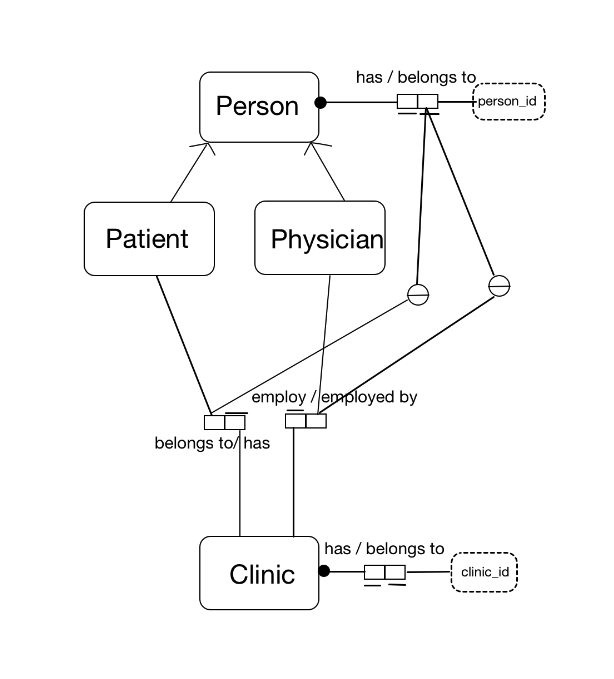
\includegraphics[width=1.0\textwidth]{Figures/LogicalModelDB1.png}
    \caption{Logical model of the OSA database - Person and Clinic}
    \label{fig:Figures/LogicalModelDB1}
\end{figure}
\begin{figure}[ht]
    \centering
    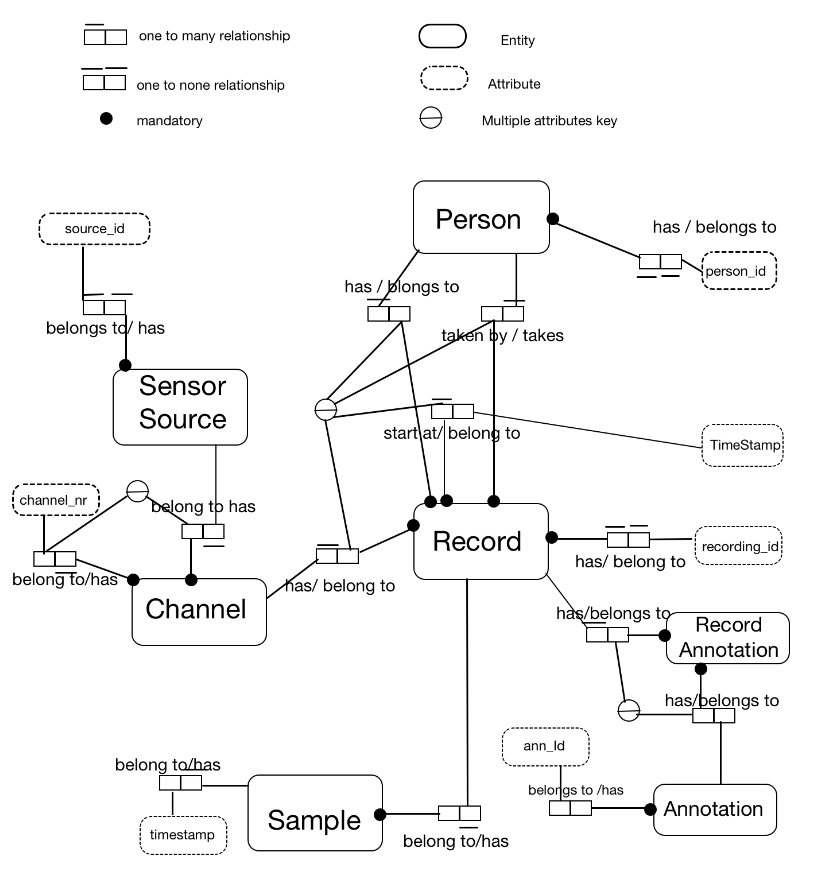
\includegraphics[width=1.0\textwidth]{Figures/LogicalModelDB2.png}
    \caption{Logical model of the OSA database - Source and Recording}
    \label{fig:Figures/LogicalModelDB2}
\end{figure}
Figure \ref{fig:Figures/LogicalModelDB1} and \ref{fig:Figures/LogicalModelDB2} presents a summary of the logical model of the database design after decomposition. In this figure, non-key attributes are hidden to maximize the abstraction.
\section{Physical data modeling}
The logical data model, which is presented in Figure \ref{fig:Figures/LogicalModelDB1} and \ref{fig:Figures/LogicalModelDB2}, is a platform independent model. This model can be implement on a workstation computer or even mobile platform as long as these platforms have a database management system. Since the thesis chooses Android operation system as a platform to implement the design, SQLite database manage system is chosen for modeling the physical data. An overview of SQLite database management system is discussed in Subsection 4.1. Subsection 4.2 presents the transformation of logical data model to physical data model.
\subsection{SQLite database management system}
As presented in SQLite site\cite{SQLITEORG}, SQLite is an embedded SQL database engine. It does not support client-server process as other database management systems do. However, other SQL database elements that are needed for this design are fully supported. They are multiple tables, indices, triggers, and views. Since all of the mentioned elements are included in a single file on disk, it is a good choice to store OSA data compared with EDF file format in terms of opening file for doing analysis or modifying.\\
SQLite has five data storage classes that can be used for the physical data modeling.
\begin{adjustwidth}{1cm}{}
•	NULL: The value is a NULL value.\\
•	INTEGER: The value of this type is a signed integer. Depend on the magnitude of the stored value, it could be 1, 2, 3, 4, 6, or 8 bytes in size.\\
•	REAL: The value of this type is a floating value following the IEEE floating point number. This type has 8 bytes in size.\\
•	TEXT: Unlike the other database management systems, SQLite has only one type for storing a text string. The encode of the text could be UTF-8, UTF-16 big-endian, or UTF-16 little endian.\\
•	BLOB: The value of this type are stored exactly as it was input.
\end{adjustwidth}
They do not use the term of “datatype”, but “storage class”, since data are dynamically stored in the system. Therefore, the data need to be converted be for storing, or using. However, at an abstract level, the two terms present data type. Hence, these terms can be used interchangeably.
\subsection{Transforming the logical data model to SQL}
As presented in Figure \ref{fig:Figures/LogicalModelDB1} and \ref{fig:Figures/LogicalModelDB2}, there are nine entities must be transformed into tables. The names of these entities are also used for tables in SQLite respectively. Attributes of the entities become columns in the tables, and the relationships now become the foreign keys.
From Table \ref{tab:PersonTypeSQL} to \ref{tab:ChannelTypeSQL} present attributes for each table with the explanation for each chosen type.
\begin{table}
\begin{center}
\begin{tabular}{ |p{4cm}|p{1.8cm}|p{6.2cm}|  }
 \hline
 \multicolumn{3}{|c|}{Person} \\
 \hline
 Columns& Data type & Explanation \\
 \hline
 person\_id& TEXT& person id can contains alphabetic character, not null\\
 name& TEXT& name is a string, can be null for anonymous\\
 city& TEXT& city is a string, can be null for anonymous\\
 phone\_nr& TEXT& phone number can contains +, can be null if not have\\
 email& TEXT& email is a string, can be null if not have\\
 gender& TEXT& gender can be a character or sometime a string, must be not null for later analysis\\
 date\_of\_birth& TEXT& date of birth is a string, must be not null for later analysis\\
 age& INT& age is an integer, can be null\\
 \hline
\end{tabular}
\end{center}
\caption{Transforming Person into SQLite table}
\label{tab:PersonTypeSQL}
\end{table}
\begin{table}
\begin{center}
\begin{tabular}{ |p{4cm}|p{1.8cm}|p{6.2cm}|  }
 \hline
 \multicolumn{3}{|c|}{Patient} \\
 \hline
 Columns& Data type & Explanation \\
 \hline
 person\_id& TEXT& foreign key to Person, not null\\
 clinic\_code\_p& TEXT& foreign key to Clinic, not null\\
 height& REAL& it must be floating number, can be null\\
 weight& REAL& it must be floating number, can be null\\
 BMI& REAL& it must be floating number, can be null\\
 other\_health\_issues& TEXT& it is a string, can be null\\
 \hline
\end{tabular}
\end{center}
\caption{Transforming Patient into SQLite table}
\label{tab:PatientTypeSQL}
\end{table}
\begin{table}
\begin{center}
\begin{tabular}{ |p{4cm}|p{1.8cm}|p{6.2cm}|  }
 \hline
 \multicolumn{3}{|c|}{Physician} \\
 \hline
 Columns& Data type & Explanation \\
 \hline
 person\_id& TEXT& foreign key to Person, not null\\
 clinic\_code\_f& TEXT& foreign key to Clinic, not null\\
 title\_in\_clinic& TEXT& it is a string, can be null\\
 \hline
\end{tabular}
\end{center}
\caption{Transforming Physician into SQLite table}
\label{tab:PhysicianTypeSQL}
\end{table}
\begin{table}
\begin{center}
\begin{tabular}{ |p{4cm}|p{1.8cm}|p{6.2cm}|  }
 \hline
 \multicolumn{3}{|c|}{Clinic} \\
 \hline
 Columns& Data type & Explanation \\
 \hline
 clinic\_code& TEXT& it can contains text, not null\\
 name& TEXT& it is a string, can be null\\
 address& TEXT& it is a string, can be null\\
 phone\_nr& TEXT& phone number can contains +, can be null if not have\\
 email& TEXT& it is a string, can be null\\
 \hline
\end{tabular}
\end{center}
\caption{Transforming Clinic into SQLite table}
\label{tab:ClinicTypeSQL}
\end{table}
\begin{table}
\begin{center}
\begin{tabular}{ |p{4cm}|p{1.8cm}|p{6.2cm}|  }
 \hline
 \multicolumn{3}{|c|}{SensorSource} \\
 \hline
 Columns& Data type & Explanation \\
 \hline
 source\_id& TEXT& it can contains text, not null\\
 source\_name& TEXT& it is a string, can be null\\
 source\_type& TEXT& it is a string, can be null\\
 \hline
\end{tabular}
\end{center}
\caption{Transforming SensorSource into SQLite table}
\label{tab:SensorSourceTypeSQL}
\end{table}
\begin{table}
\begin{center}
\begin{tabular}{ |p{4cm}|p{1.8cm}|p{6.2cm}|  }
 \hline
 \multicolumn{3}{|c|}{Record} \\
 \hline
 Columns& Data type & Explanation \\
 \hline
 recording\_id& INT& unique long int from the system when created\\
 source\_id& TEXT& foreign key to SensorSource, not null\\
 person\_collect& TEXT& foreign key to Person, not null\\
 person\_owner& TEXT& foreign key to Person, not null\\
 timestamp& INT& Unix time when the recording is started, not null\\
 description& TEXT& can be the applied position on the body, can be null\\
 recording\_fragment\_duration& INT& duration of one fragment, not null\\
 frequency& REAL& collected at frequency, can be null\\
 pre\_filtering& TEXT& applied filtering on this record, can be null\\
 used\_equipment& TEXT& other used equipment name, can be null\\
 EDF\_reverved\_for\_recording& BLOB& reserved for EDF, byte array, can be null\\
 \hline
\end{tabular}
\end{center}
\caption{Transforming Record into SQLite table}
\label{tab:RecordTypeSQL}
\end{table}
\begin{table}
\begin{center}
\begin{tabular}{ |p{4cm}|p{1.8cm}|p{6.2cm}|  }
 \hline
 \multicolumn{3}{|c|}{RecordFragment} \\
 \hline
 Columns& Data type & Explanation \\
 \hline
 recording\_id& INT& foreign key to Record, not null\\
 recording\_fragment\_index& INT& the fragment index, not null\\
 recording\_fragment\_timestamp& INT& Unix time, when it is created, not null\\
 \hline
\end{tabular}
\end{center}
\caption{Transforming RecordFragment into SQLite table}
\label{tab:RecordFragmentTypeSQL}
\end{table}
\begin{table}
\begin{center}
\begin{tabular}{ |p{4cm}|p{1.8cm}|p{6.2cm}|  }
 \hline
 \multicolumn{3}{|c|}{Sample} \\
 \hline
 Columns& Data type & Explanation \\
 \hline
 recording\_id& INT& foreign key to Record, not null\\
 channel\_id& INT& foreign key to Channel, not null\\
 recording\_fragment\_index& INT& foreign key to RecordFragment, not null\\
 sample\_timestamp& INT& Unix time, when it is created, not null\\
 sample\_value\_annotation& TEXT& it is a string, can be null\\
 sample\_value\_float& REAL& it is a float number, can be null\\
 \hline
\end{tabular}
\end{center}
\caption{Transforming Sample into SQLite table}
\label{tab:SampleTypeSQL}
\end{table}
\begin{table}
\begin{center}
\begin{tabular}{ |p{4cm}|p{1.8cm}|p{6.2cm}|  }
 \hline
 \multicolumn{3}{|c|}{Channel} \\
 \hline
 Columns& Data type & Explanation \\
 \hline
 channel\_id& INT& unique number that is automatic created by system when channel is created, not null\\
 source\_id& TEXT& foreign key to SensorSource, not null\\
 channel\_nr& INT& numerical order, not null\\
 channel\_name& TEXT& name of channel, not null\\
 metric& TEXT& metric, not null\\
 transducer\_type& TEXT& it is string, can be null\\
 physical\_maximum& REAL& physical maximum, can be null\\
 physical\_minimum& REAL& physical minimum, can be null\\
 digital\_maximum& INT& digital max, can be null\\
 digital\_minimum& INT& digital min, can be null\\
 EDF\_channel\_reserved& BLOB& EDF reserved\\
 \hline
\end{tabular}
\end{center}
\caption{Transforming Channel into SQLite table}
\label{tab:ChannelTypeSQL}
\end{table}
SQLite code for creating Channel table is presented in Listing \ref{listing:SQLChannel}, creating code for other tables can be found in Appendix XX.
\begin{code}[ht]
\begin{lstlisting}
    CREATE TABLE CHANNEL(
	   CHANNEL_ID              INT PRIMARY KEY,
	   SOURCE_ID               TEXT NOT NULL,
	   CHANNEL_NR              INT NOT NULL,
	   CHANNEL_NAME            TEXT NOT NULL,
	   TRANSDUCER_TYPE         TEXT,
	   METRIC                  TEXT,
	   PHYSICAL_MAX            REAL,
	   PHYSICAL_MIN            REAL,
	   DIGITAL_MAX             INT,
	   DIGITAL_MIN             INT,
	   EDF_CHANNEL_RESERVED    BLOB,
	   UNIQUE (CHANNEL_NR ,SOURCE_ID),
       FOREIGN KEY(SOURCEID) REFERENCES TABLE_SENSOR_SOURCE(SOURCE_ID)
	);
\end{lstlisting}
\caption[SQLite code for creating table Channel]{SQLite code for creating table Channel}
\label{listing:SQLChannel}
\end{code}
Figure \ref{fig:Figures/FinalTable} presents the final physical database model of the database system.
\begin{figure}[ht]
    \centering
    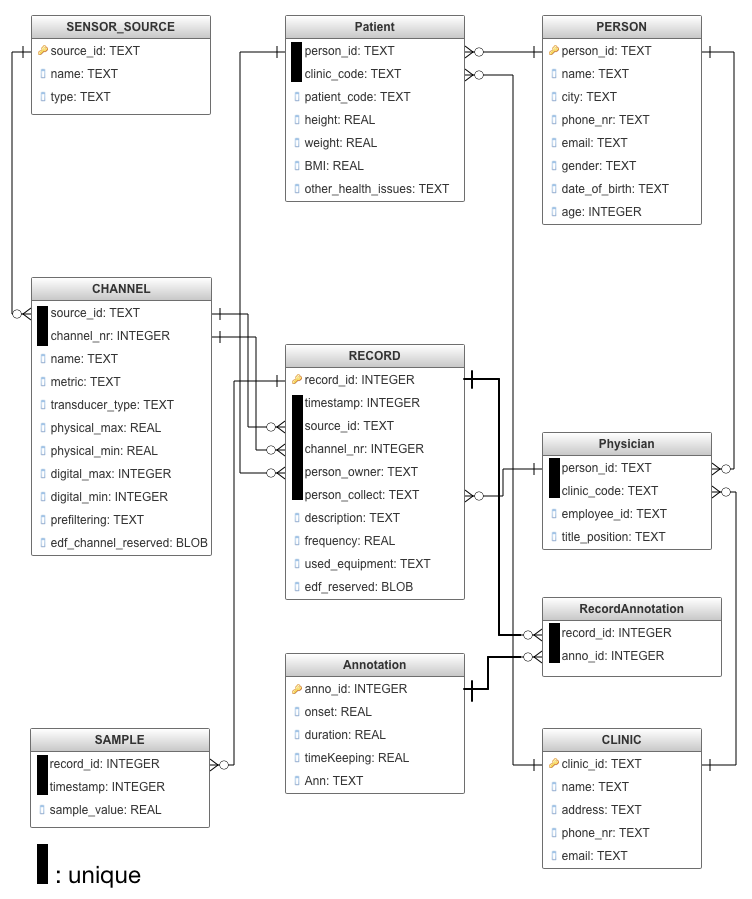
\includegraphics[width=1.0\textwidth]{Figures/FinalTable.png}
    \caption{Physical database model}
    \label{fig:Figures/FinalTable}
\end{figure}






 
\chapter{Implementation}
Patients, physicians, and researchers do not only want to store OSA signal into a relational database system, but also want to do data analysis based on the collected data. Computing ability and storage capability of mobile devices are huge improved, and the users would like to store and perform data analysis on these devices. Therefore, a database system application on mobile platform for the designed database model in Chapter 4 needs to be taken into considering. The implementation mainly focuses on developing sensor wrappers on Android operative system for the designed database, and writing SQLite codes to do data analysis. Hence, other functions such as GUI interactions between users and the application, visualizing data on graph, etc., are minor. It is to say, not all of features are implemented, therefore, the implementation is a proof-of-concept. This chapter presents a traditional software engineering approach, in which, the waterfall process model approach is mainly used for developing the application. It is because the process activities can be separately presented (requirements specification, software design, implementation and so on). Incremental development approach is useful when the requirements changes frequently, and new functions need to be added to the previous version. Hence, it is not suitable for the OSA database system, since the data requirements are stable. At the time of the writing, the OSA data are not stored in any relational databases. Instead, each clinic has their own file format for storing the data. The users can either use the provided tools from these clinic, or ask for a general format file (EDF format) in order to do data analysis. Therefore, reuse-oriented software engineering approach cannot be used, since the database application must be developed from scratch than integrated into an exist system.\\
In this chapter, functional and non-functional requirements of the users are carefully analyzed. These requirements are presented in Section 5.1; they are supplementary to the discussed requirements in Chapter 4. Section 5.2 presents an abstract model of the database system application and architectural models with respect to real-time wrapper and EDF wrapper. Possible data mining algorithms are also discussed in this section. Section 5.3 presents an Android specific implementation of the discussed models and the implementation of possible data mining algorithms.
\section{Requirements for database application}
\begin{table}
\begin{adjustwidth}{-1.5cm}{}
\begin{center}
\begin{tabular}{ |p{2.4cm}|p{5.5cm}|p{3.3cm}|p{4.3cm}|}
 \hline
 User requirements definition& System functional requirements& System non-functional requirements& Structured specifications\\
 \hline
 The application must reuse CESAR acquisition tool to collect data from BITalino.&
 1. System must open a port for that CESAR acquisition tool can connect and send data.\newline
 2. System must follow CESAR package formats for that the data can be correctly collected.\newline
 3. System must let the users fill out the requirement fields for patient and clinic before storing a record into database system.\newline
 4. System must support multiple connections.&
 - Product: usability, performance, space, reliability\newline
 - Organization: Android operative system (6.0)\newline
 - External: must follow the protection of personal data of patient&
 - Input: metadata and data packages from CESAR\newline
 - Source: BITalino\newline
 - Output: store metadata and data to database system, and may plot them to graph\newline
 - Place: fragment server application and fragment real-time visualization\\
 \hline
 The application must support importing and exporting EDF files.&
 1. The user can freely choose a EDF file to import, and import progress must be showed.\newline
 2. The user can partially import an EDF file by click stop button, in case they do not want to wait.\newline
 3. System must support fully or partially export. That is, the user can choose from time – to time when exporting.\newline
 4. The user can choose which channels they want to export.&
 - Product: usability, performance, space, reliability\newline
 - Organization: Android operative system (6.0)\newline
 - External: must follow the protection of personal data of patient&
 - Input: EDF header and EDF data record\newline
 - Source: EDF file\newline
 - Output: store/export EDF header and data record to database system/EDF file\newline
 - Place: fragment EDF reader and fragment EDF exporter\\
 \hline
 Data analysis can be perform by using the application.&
 1. The system must support raw query, in which the users can write SQL queries to retrieve whatever they want.\newline
 2. The system must provide some mining functions to detect OSA signal.&
 - Product: usability, performance, space, reliability\newline
 - Organization: Android operative system (6.0), SQL query language&
 - Input: data in database system\newline
 - Source: database system\newline
 - Output: result from SQL, or OSA detection\newline
 - Place: mining fragment\\
 \hline
 Collected data could be visualized in real-time data, or replay from the stored data.&
 1. The user can visualize data on a graph view.\newline
 2. Channels can be freely choose to visualize to do comparison.&
 - Product: usability, performance, space, reliability\newline
 - Organization: Android operative system (6.0)&
 - Input: BITalino or database\newline
 - Source: BITalino or database\newline
 - Output: graphic view\newline
 - Place: fragment real-time/replay visualization\\
 \hline
 Annotations could be added manually to a certain source.&
 Annotations could be manually added and stored while visualizing sources.&
 - Product: usability, performance, space, reliability\newline
 - Organization: Android operative system (6.0)&
 - Input: data in database\newline
 - Source: database\newline
 - Output: annotations from users are stored in database system\newline
 - Place: fragment replay visualization\\
 \hline
\end{tabular}
\end{center}
\end{adjustwidth}
\caption{A summary of the database system application requirements}
\label{tab:userrequirementAPP}
\end{table}
This section presents and analyzes the specific requirements of the users as well as the database application system. The analysis results provide the foundation for designing the data model and the implementation for the application.\\
User requirements are usually presented as statements. These statements are in natural language, and are about services that the system is expected to provide to the users, and constrains for the services. On the other hands, system requirements present a list of system requirement specifications for each user requirement statement. In short, the users define the requirements, while the system specifies in detailed the services it provides, inputs and outputs, functional and non-functional requirements, etc., for each of defined requirement.\\
Functional requirements are statements of services the system should provide, how the system should react to particular inputs, and how the system should behave in particular situation \cite{INF1050BOOK}. On the other hands, non-functional requirement are constraints on the services or functions offered by the system. They are included timing constrains, constrains on the development process, and constraints imposed by standards \cite{INF1050BOOK}.
Table \ref{tab:userrequirementAPP} presents the requirements of the database system application. In which, each user requirement defines the services the system must provide. Correspondingly, the system requirements clearly explain how the system must behave to satisfy the user requirement. These system requirements are presented in forms of functional requirements and non-functional requirements, and structured specifications of the requirements. “Place” in structure specifications column presents which function groups the requirements belong to. By grouping requirements in a group of functions, it is easier to design and implement. Function groups are illustrated in Figure \ref{fig:Figures/OSADBSContext}.
\begin{figure}[ht]
    \centering
    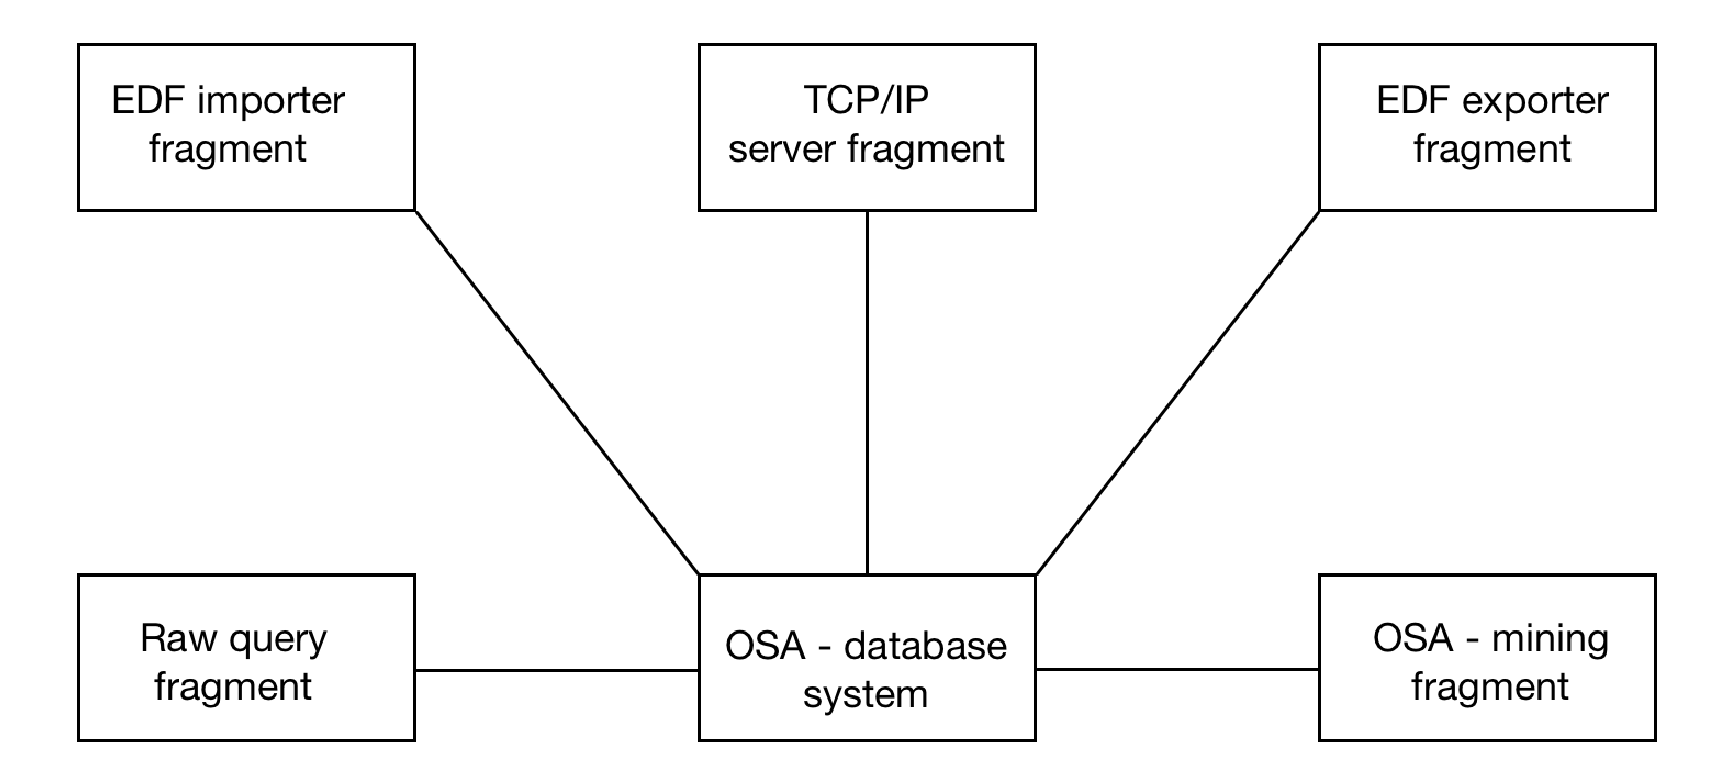
\includegraphics[width=1.0\textwidth]{Figures/OSADBSContext.png}
    \caption{The context of the OSA database system application}
    \label{fig:Figures/OSADBSContext}
\end{figure}
The first two and the last three requirements in Table \ref{tab:userrequirementAPP} are respectively corresponded to “what it must contain” and “what the database is to be used for” presented in the database modeling chapter. In other words, the database application needs to be implemented two wrappers that collect data from CESAR acquisition tool and EDF/EDF+ file formats, then the collected data can be used for analyzing, visualizing, or modifying. Since the mainly focus of the thesis are collecting data and data analysis, therefore visualizing and modifying are added as helper functions.\\
The first two user requirements illustrate that the system must support collecting samples from BITalino by using CESAR acquisition tool, and importing EDF/EDF+ data. As presented in Chapter 3, for collecting samples from CESAR acquisition tool, the system first establishes a TCP/IP connection to the tool, then the metadata and data packages are sent to the system. The structure of these packages are well documented, and have been discussed in Chapter 3. The user can also use multiple acquisition tools to collect sample, hence the application must support multiple connections as well. Since CESAR acquisition tool does not send the information of the clinic and patient, the information must be manually filled by the user before recording samples. CESAR acquisition tool provides data in real-time, therefore the system must operate with respect to the given non-functional requirements presented in Table \ref{tab:userrequirementAPP}. Likewise, for importing and exporting EDF/EDF+ files, the system must follow the structure of the EDF/EDF files which are also well discussed in Chapter 3. Since the files can be very large, the system must satisfy the non-functional requirements when importing and exporting.\\
As mentioned earlier, visualizing and modifying are not the main focus of the thesis. They are added to the database system application as helper functions to help the user have a better view on the collected data. Therefore, they are implemented as proof-of-concept and “enough for using”. For the analysis requirements, a raw query function is useful when analyzing the data. However, in term of security, this is quiet dangerous action. In the top 10 vulnerabilities, SQL injection stands on the top of the list\cite{OWASP}. In this case, the risk does not come from stealing of sensitive information, or compromising the database. It is dangerous if the researchers accidentally perform queries that can result the database system corrupted, such as deleting a column in a data table, drop a table, etc. Filter out vulnerable queries is a topic for researchers who are interested in database security. Hence, to filter out vulnerable queries is not in scope of the thesis. An assumption is made that the users have the knowledge on database system, and they do not perform any vulnerable queries. The system must also provide some of possible mining algorithms that are used for detecting OSA signal.
\section{System modeling}
As presented in Figure \ref{tab:userrequirementAPP}, the context of the OSA database system consists of importing, exporting and analyzing data. Data sources, in which the system collects data from, can be divided into two groups. Sources that connect to the database system via TCP/IP protocol are real-time sources. On the other hands, non-real-time sources are from EDF/EDF+ files. Data analysis are only performed on the stored data. Currently, the system does not support real-time analysis, since the goals of the system are collecting raw data for future analysis. That is, the collected data are used as the inputs for many different analysis algorithms than the possible mining methods presented in this thesis. However, real-time OSA data analysis is good to be considered, and an exciting topic for researchers who are interested in online analytical processing.\\
Subsection 5.2.1 presents real-time wrapper modeling, in which, some real-time attributes are taken into considered, and how the TCP/IP server fragment is modeled. Subsection 5.2.2 presents the modeling for non-real-time wrapper, in which EDF importer fragment and EDF exporter fragment are carefully modelled. Subsection 5.2.3 discusses training set, OSA pattern, and possible mining algorithms can be used for detecting OSA signal at abstract level.
\subsection{Real-time wrapper}
When choosing the appropriate real time sensor sources, several factors should be considered, such as the quality of signal, mobility, how many channels can it observe, which protocol it uses to send data sample, etc. The BITalino platform is chosen as sensor source after carefully considering the pros and cons of it in Chapter 3.\\
In terms of real-time data stream source, the system has to deal with data stream management problems. The thesis targets at a solution to store the OSA bio-signals, and it does not address data stream management system issues, where the queries need to be apply on the data stream. Instead, some general real time factors need to be seriously considered when designing the database system. These factors are arrival rate, timestamp, physical resource, one-time read data, data stale or imprecise, and unpredictable data arrival. When the incoming rate is high, it might be a problem to store all the data, because of the limitation of the mobile platform. Even on a stationary computer, storing data streams could be a problem and needs to be considered.\\
To choose a suitable solution for manage the arrival rate of the data stream, it is good to review and discuss how the data stream management system (DSMS) deal with real-time data stream problems. Due to the unboundedness of the data stream, it is essential to capture the stream into small slices which is called windows. To manage the data stream, DSMS uses window models, in which the models are based on the direction of movement of the endpoints, that are fixed window, sliding window, and landmark window. As the name of the window models, the fixed window has a fixed amount of samples or time interval. The sliding window contains the data from now up to a certain range in the past. The landmark window, on the other hand, contains the data from the beginning until now. The window size can be either physical/time-based or logical/count based. Figure \ref{fig:Figures/windows} presents an overview of the fixed window and sliding window.
\begin{figure}[ht]
    \centering
    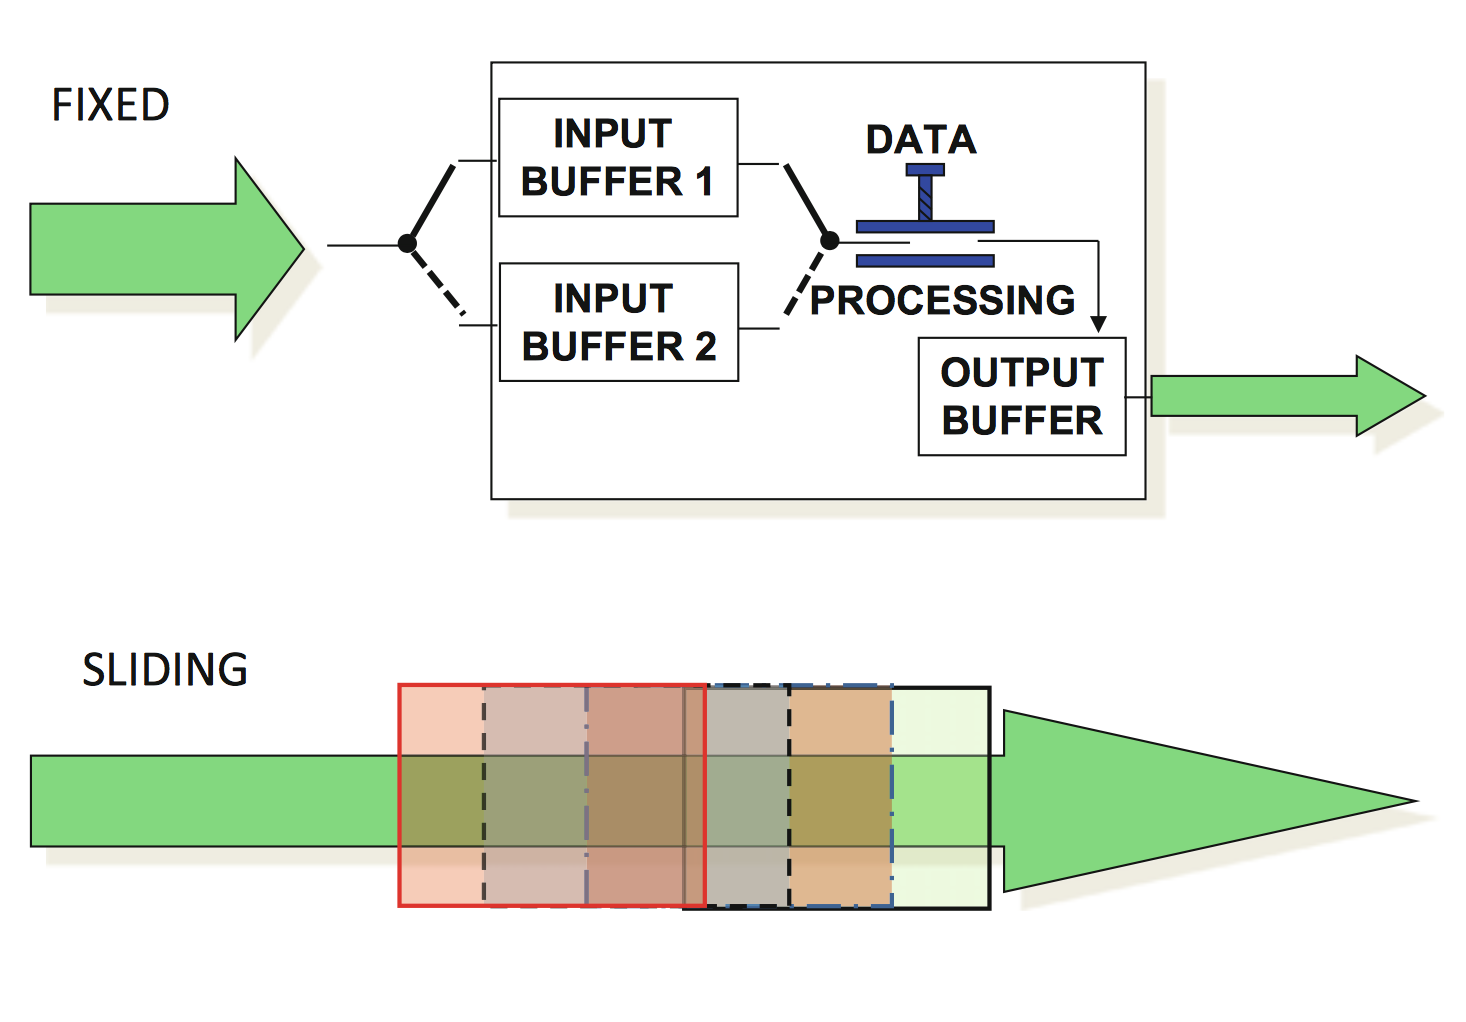
\includegraphics[width=0.6\textwidth]{Figures/WINDOWDSMS.png}
    \caption{Example of fixed and sliding windows \cite{DSMS_WINDOW}}
    \label{fig:Figures/windows}
\end{figure}
When a sample arrives, it is updated either immediately (eager processing) or when the window is full (lazy/batch processing).\\
Tasks of the system are to store the raw data samples as well as to display these samples to a graph view with respect to the users’ requirements. To ensure that the tasks are well performed, the system uses two buffers which functioned as windows in DSMS. It is to say, the first buffer is a fixed window, count based, and batch processing, that is used for collecting samples for the database. The second buffer is a sliding window, count (or time) based, eager processing, that is used for collecting samples for graphic view. By using these two buffer, the system ensures that the overhead of writing to database is minimized (by using batching processing), while the performance increases (by using eager processing).\\
If the order of the samples plays an important role for later analysis, the timestamp must be explicit (timestamp from data source). Otherwise, the implicit timestamp (system time) can be used. The CESAR acquisition tool provides the timestamp in each sample object. However, the timestamp is pre-converted and need to be handled before using for plot view. It is an overhead for converting timestamp for each sample. Moreover, the system uses local network for sending samples, and the assumption is made that the delay in network and order of the samples are acceptable. Therefore, the implicit timestamp is considered a better solution than the explicit timestamp with respect to system overhead, hence the performance is improved. A comparison between these timestamp is presented in Appendix XX.\\\\
\textbf{Server thread}\\
The collector of CESAR acquisition tool offers two methods for that the database application can collect data from it. The collector can either save data to a text file or send them to a given server IP and port address by using TCP/IP protocol. Since the database system application wants to have real-time data from BITalino, it must open a port to collect data. As presented in requirement section, the system must support multiple connections, because the user may use multiple sensor source to monitor the body. Therefore, multiple threads system must be implemented. Each thread manages one sensor source. The main thread therefore just waits for connections, creates and hands in necessary information to the new created thread, then starts the new thread. The main thread must have a way to manage the created threads for that the users can choose a source they want to interact with from the connected list. A Unified Modeling Language (UML) activity diagram is used for illustrating how the main thread works as presented in Figure \ref{fig:Figures/ServerActivity}. UML is a famous and widely used modeling language, however, a short explanation on the used annotations is needed to make the figures easier to understand. In UML activity diagram, a filled circles indicates the start of a process. Activities are presented by rectangles with round corners. Arrows present the flow of work between activities. Annotations on the arrow indicate the condition when the work flow is taken. A filled circle inside another circle indicates the end of the process.\\
\begin{figure}[ht]
    \centering
    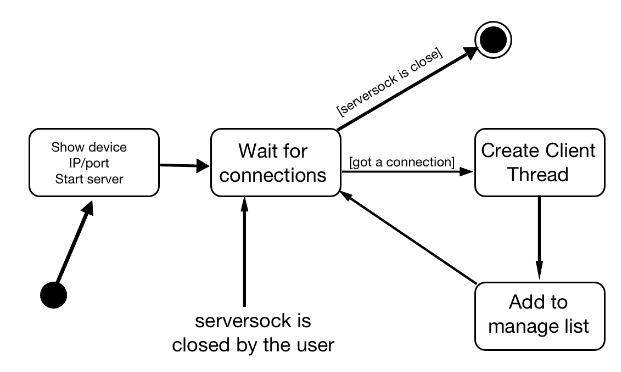
\includegraphics[width=1.0\textwidth]{Figures/ServerActivity.png}
    \caption{Process model of server thread}
    \label{fig:Figures/ServerActivity}
\end{figure}
\textbf{Client thread}\\
Most of the jobs of the wrapper are handled in the client thread. Once a client thread is created, it waits for arrival data, then pushes to database or adds to graphical view if these actions are flagged. Data packages from CESAR acquisition tool are well discussed in Chapter 3, in which a metadata package is sent first to identify the sensor source, then the source keeps sending its data via the connection between the database system application and the acquisition tool. As explained in the real-time characteristics, the client thread must share two buffers with the other threads. The first buffer is used for storing samples to the database, and the second buffer is used for showing samples on a graphic view. However, these buffers are initialized only if the corresponded flags are flagged. That is, arrival samples are thrown if the users do not want to store or visualize them. Figure \ref{fig:Figures/ClientThreadAc} presents a possible implementation of the client thread by using a UML activity diagram.
\begin{figure}[ht]
    \centering
    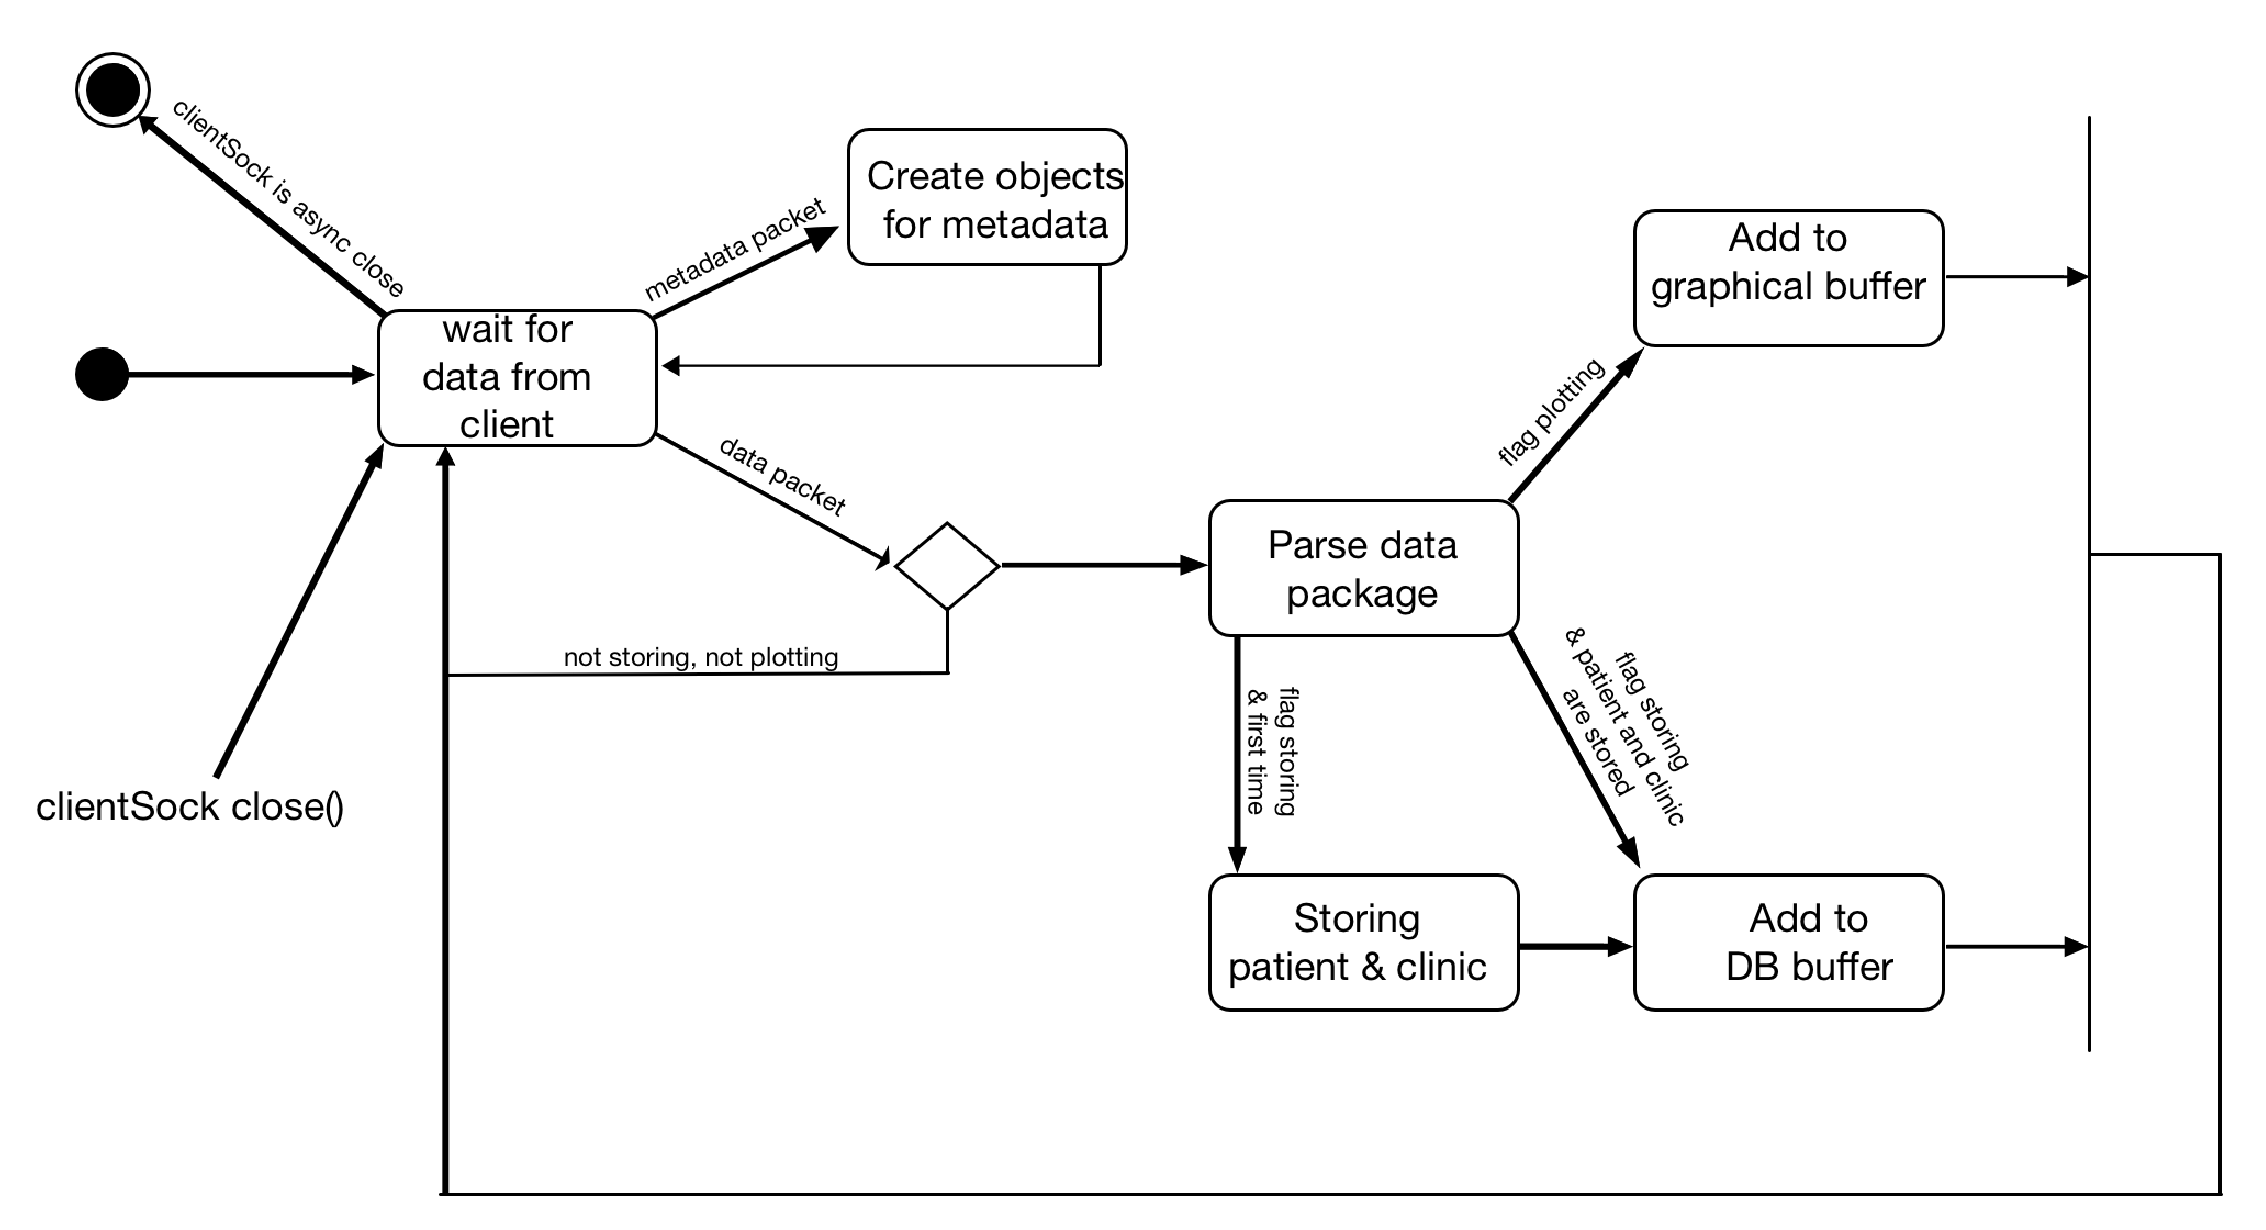
\includegraphics[width=1.0\textwidth]{Figures/ClientThreadAc.png}
    \caption{Process model of client thread}
    \label{fig:Figures/ClientThreadAc}
\end{figure}
As illustrated in the requirements, the system must be reliable and have a good performance. That is, no samples data are lost under recording, and the visualization must not be frozen. To satisfy these requirements, two different buffer management methods are used. A buffer, which is used for storing samples, maintains a list of fixed number of samples (it is to say, a record fragment), and a thread. The thread takes a full record fragment to store into the database, or waits for available record fragments if the list is empty. Since SQLite can perform about 50,000\cite{SQLITEORG_INSERT} insert statements per second, while the maximum number of samples BITalino can delivery is 1000 samples per second (1000Hz), the algorithm for this buffer is therefore satisfied the non-functional requirement (reliable). The second buffer can be implemented by using the algorithm from Producer and Consumer problem, in which the client thread is the producer, and a thread that update the graphic view is the consumer. However, this buffer is used as a sliding window, therefore a simpler solution can be used. That is, each time client thread adds a sample to a buffer list, it removes the oldest sample if the buffer is full. After that, a graphic view thread is notified to refresh the plot view.\\
Figure \ref{fig:Figures/ThreadsDBPlot} presents how the sever thread, client thread, database, and graphic view connect to each other’s.
\begin{figure}[ht]
    \centering
    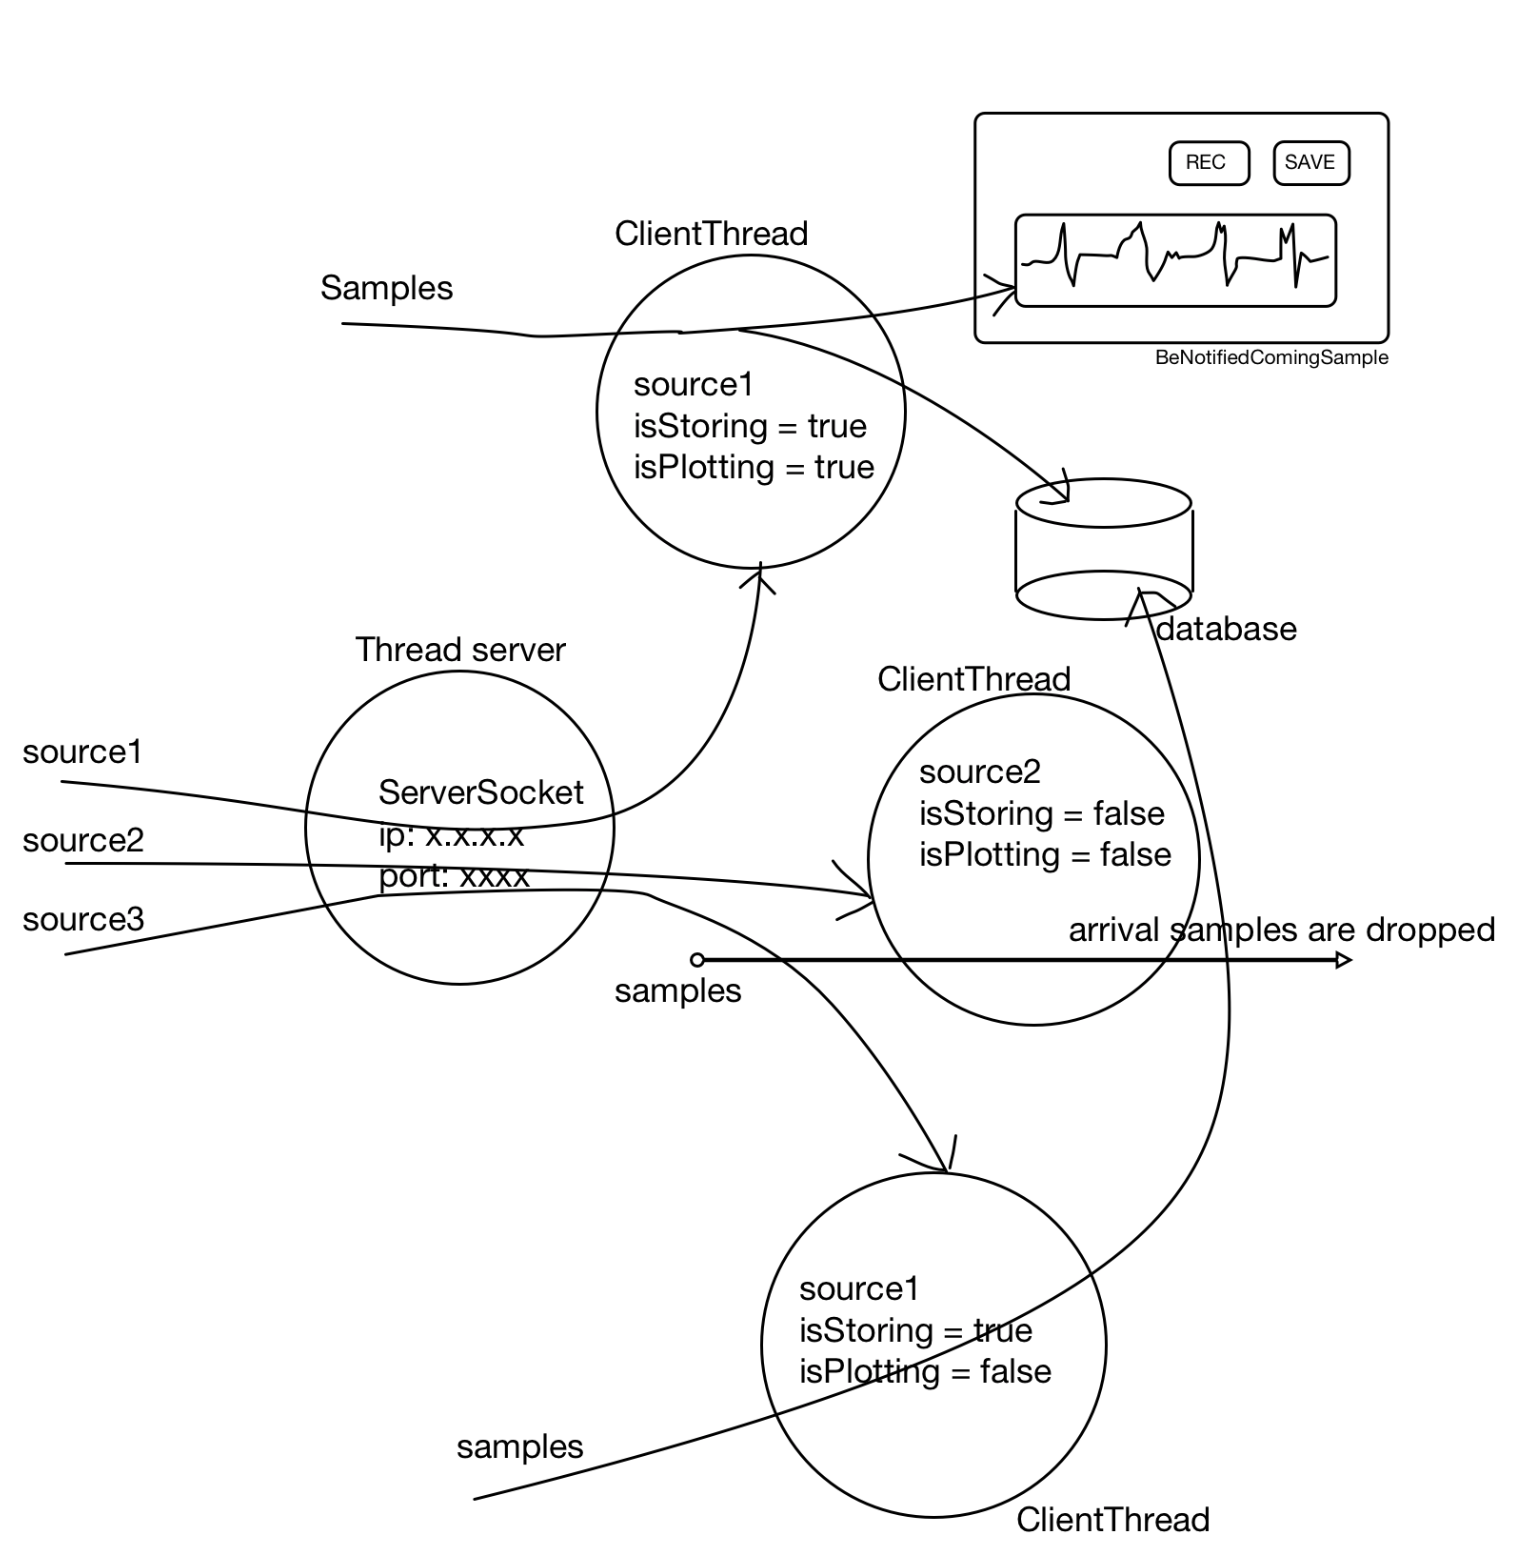
\includegraphics[width=1.0\textwidth]{Figures/ThreadsDBPlot.png}
    \caption{High level design of real-time wrapper}
    \label{fig:Figures/ThreadsDBPlot}
\end{figure}
\subsection{Non real-time wrapper}
Diverse data sources are essential in research. Using multiple sources of data in research often produces more accurate results and more objective values than using a single data source. There are many trustworthy sources that can be used for OSA data analysis. One of the sources that is chosen in this thesis are the Physionet sensor databases, which have been described in Section 3.1.2. The other non-real time source that the system collects data from, is NOX-T3 sensor source system. Theoretically, this source can be used as a real time sensor source. Although Nox-medical has an Android application, which is only support NOX-A1-PSG at the time of this writing, to collect samples from their devices, the NOX-T3 device neither provide any API for mobile platform, nor any documents that describe how to collect samples from the device as BITalino does. As mentioned earlier, it is very difficult to manage diverse sources when they have their own format. Fortunately, the problem is solved by using an EDF or an EDF+ file format to share data between source owners. The formats are fully described in Section 3.2.2 with respect to why they are introduced, what information these file contain, and how to use them. Therefore, the system is designed in the way that is opened for all of the sensor sources, as long as these sources can export their data to an EDF or EDF+ file format. In other words, the system only accepts source files in EDF form.\\
An EDF file can be very large, and can excess the main memory size. Hence, to satisfy the performance and robustness, the system should neither keep all the data in memory, nor call the database insert function for each sample. The problem could be solved by using the idea from real time sensor source. In other words, the system uses the concept of a window model, lazy update (batch processing) to solve the memory problem with the non-real time source.\\
Physionet databases and NOX-T3 sensor source can be used as non-real-time sources, because both of them provide a function to export their bio-signal data to EDF. “mit2edf” is a function from physiotools provided by Physionet. This function is used for converting between EDF and WFDB-compatible formats. NOX-T3 provides a graphic, step by step, and user friendly way to export their data to EDF.
\subsubsection{EDF importer}
As introduced in Chapter 3, EDF is one of the standardized data formats for bio-signals that used for storing and exchanging multichannel biological and physical signals. There is many tools and open source codes which can be used for reading a EDF file. Different tools have different goals when reading the EDF file. Most of them parse the samples to a graphical view and an annotations list, the others try to convert samples into text files that contain information for each channel and the record. EDF browser and EDF library\cite{EDFLIB} are one of the most famous used tools to view and parse EDF files. The performance of the tools is quite good since they are written in C code. Another open source tool that can be used for parsing EDF files to text files is Java-parser for EDF format\cite{EDF4J}. As the tool named, it is written in Java code, hence, the performance when parsing EDF file is poorer compared with EDF library. Since EDF/EDF+ file formats are well documented, it is easy to write a parsing tool. As discussed, different tools have different purposes when parsing EDF files. Since the one of the main goals of EDF file format is used for exchanging biological data, the EDF files need to be parsed into the received system data structure. Many parsers try to load the whole EDF file into main memory before converting. As discussed, the EDF file can be extremely large, the parsers therefore crash; Java-parser for EDF format is one them.\\
There is no need to “reinventing the wheel” rather using them in a smart way. Since in the designed database system, each bio-object is stored in a separate table. Therefore, the EDF importer can use the functions in an EDF library to read the EDF files. The information, which are read from EDF, are stored into the corresponded tables. In case the used library tries to read the whole EDF file into memory, an optimization, which is multiphase read, need to be used. Figure \ref{fig:Figures/EDFImporter} presents a UML activity diagram which explains how a EDF file can be read into the database without memory problem.
\begin{figure}[ht]
    \centering
    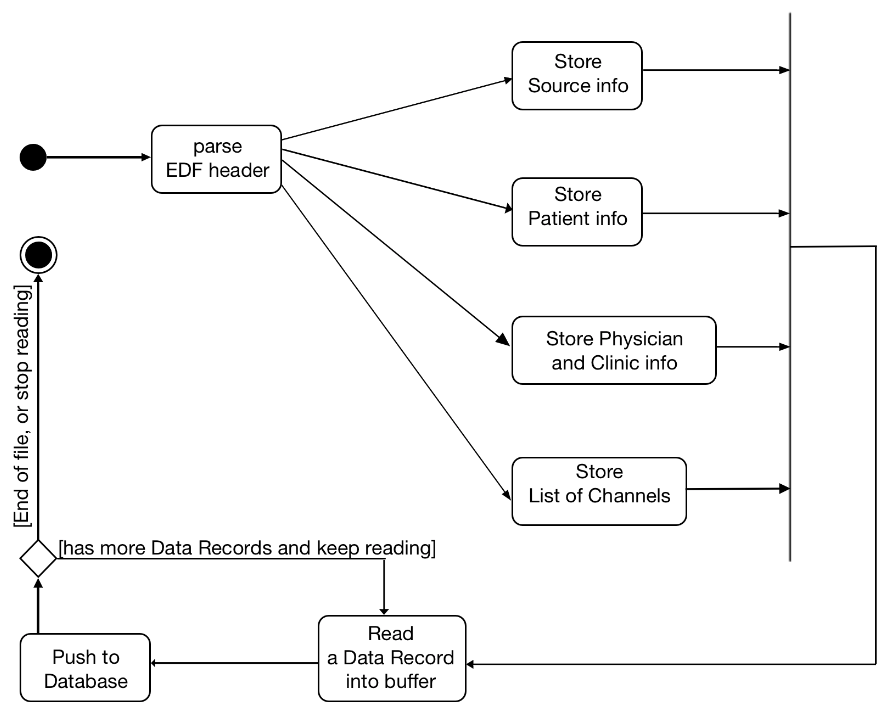
\includegraphics[width=1.0\textwidth]{Figures/EDFImporter.png}
    \caption{Process model of EDF importer}
    \label{fig:Figures/EDFImporter}
\end{figure}
\subsubsection{EDF exporter}
Sharing data is essential in researching. Therefore, the system must export its data into a standardized data formats for bio-signals, a EDF file. On the other hands, the system targets to be implemented on a mobile platform, where resources are very limited. Exporting data and saving it in external storage places is vital to satisfy non-functional requirements, where the collected data must not be lost when the storage capability of the mobile devices exceed. There is no need to export the whole source of data to a EDF file, some of channels or samples are exported for special needs. For example, there is a project, in which researchers or physicians need only samples from ECG channel, it does not make sense if the EDF file contains samples for the other non-relevant channels. Furthermore, if a project needs to analyze all samples which collected on nighttime, the added daytime samples are waste of not only the storage, but also time to parse the EDF file when using. Therefore, the system must let the users choose which channels and periods they want to export. As discussed in the non-functional requirements for EDF importer and exporter, the information of the patient must follow the protection of personal data law. That is, the patient must be exported as anonymous, otherwise there must be an agreement of the patient. Figure \ref{fig:Figures/EDFExporter} is a UML activity diagram that illustrate how data are exported into a EDF file.
\begin{figure}[ht]
    \centering
    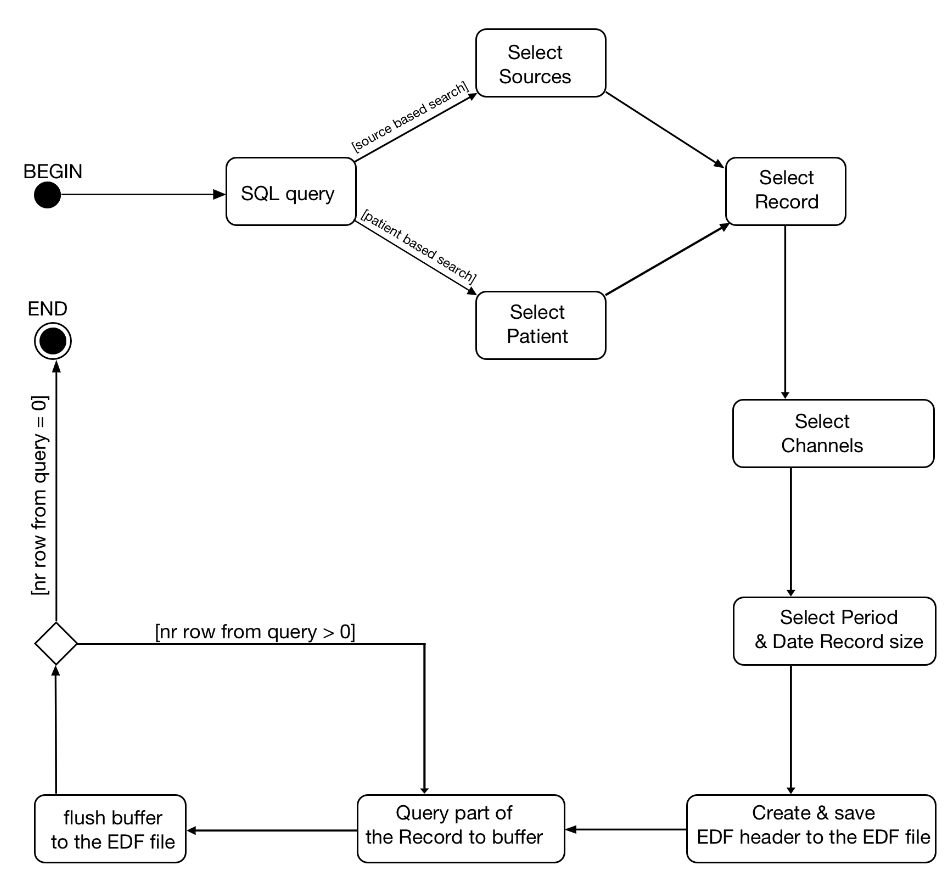
\includegraphics[width=1.0\textwidth]{Figures/EDFExporter.png}
    \caption{Process model of EDF exporter}
    \label{fig:Figures/EDFExporter}
\end{figure}
\section{Android specific design and implementation}
\subsection{Graphical user interface}
\subsection{CESAR wrapper}
\subsection{EDF wrapper}
\subsection{Mining}
\subsubsection{Workload generator}
\subsubsection{OSA pattern and trained sets}
\subsubsection{Possible mining algorithms}
\textbf{Decision tree}\\
\textbf{K-nearest neighbor}\\
\textbf{Support Vector Machine}\\
\textbf{Artificial Neural Network} 
\chapter{Evaluation}
\chapter{Conclusion}

%----------------------------------------------------------------------------------------
%	THESIS CONTENT - APPENDICES
%----------------------------------------------------------------------------------------

\appendix % Cue to tell LaTeX that the following "chapters" are Appendices

% Include the appendices of the thesis as separate files from the Appendices folder
% Uncomment the lines as you write the Appendices

\chapter{An Appendix}

% Appendix B

\chapter{Results of the experiments}
\label{AppendixB}
This appendix presents the results from the experiments in Evaluation chapter. For each experiment, a graph of percentage of CPU usage is presented. Figures of the percentage of power are also presented if any. The other results are found on the github.com by following this link \href{https://github.com/vietttifi/MasterThesisUiO/tree/master/MSc%20Latex/Experiments%20Results}{https://github.com/vietttifi/MasterThesisUiO/tree/master/MSc\%20Latex/Experiments\%20Results}.
\section{Real-time data collection experiment}
\begin{figure}
    \centering
    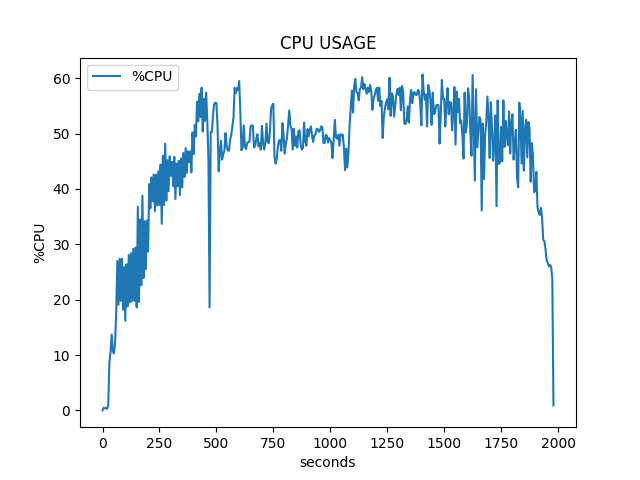
\includegraphics[width=1.0\textwidth]{Figures/StressTest.png}
    \caption{CPU usage under stress test}
    \label{fig:Figures/REALTIME_RESULT}
\end{figure}
\section{Overnight experiment}
\begin{figure}
    \centering
    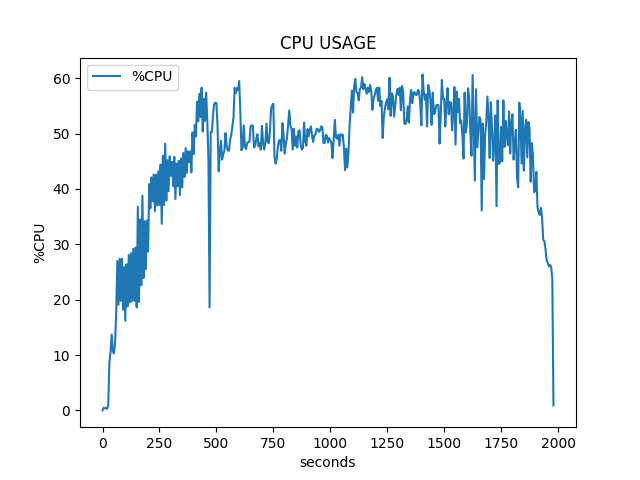
\includegraphics[width=1.0\textwidth]{Figures/StressTest.png}
    \caption{CPU usage under stress test}
    \label{fig:Figures/OVERNIGHT_RESULT}
\end{figure}
\section{EDF import}
\begin{figure}
    \centering
    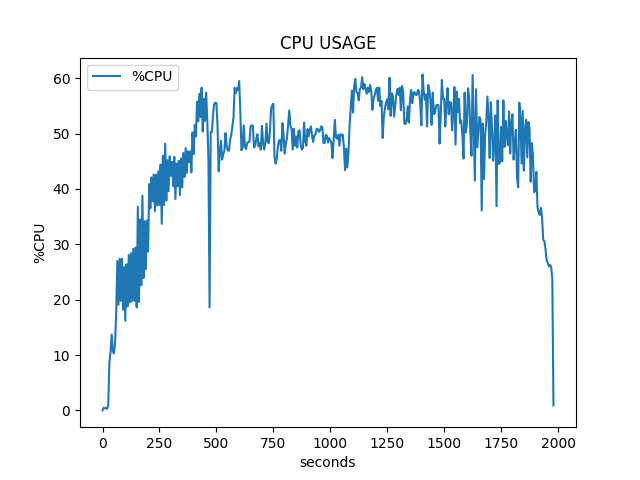
\includegraphics[width=1.0\textwidth]{Figures/StressTest.png}
    \caption{CPU usage under stress test}
    \label{fig:Figures/EDFIMP_RESULT}
\end{figure}
\section{EDF export}
\begin{figure}
    \centering
    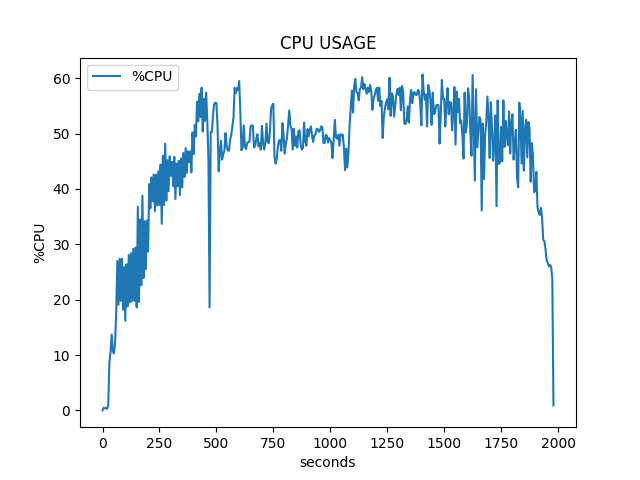
\includegraphics[width=1.0\textwidth]{Figures/StressTest.png}
    \caption{CPU usage under stress test}
    \label{fig:Figures/EDFEXP_RESULT}
\end{figure}
\section{Querying data experiment}
\begin{figure}
    \centering
    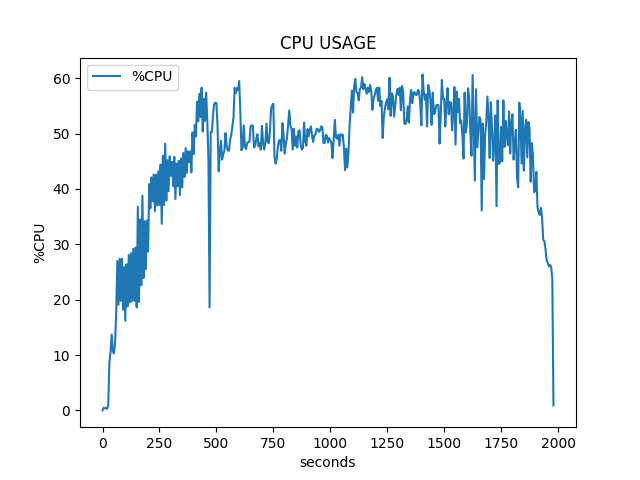
\includegraphics[width=1.0\textwidth]{Figures/StressTest.png}
    \caption{CPU usage under stress test}
    \label{fig:Figures/QUERYING_RESULT}
\end{figure}

% Appendix C

\chapter{Python code for parsing CPU usage} % Main appendix title
\label{AppendixC}
\section{How to parse the output from Busybox}
\begin{minipage}{\linewidth}
\begin{lstlisting}[caption={A sample of five seconds fragment output from the text file}, label = {listing:BUSYBOXTOPTEXT}, captionpos=b, basicstyle=\ttfamily\footnotesize]
[H[JMem: 2720896K used, 39068K free, 0K shrd, 2496K buff, 537K cached
CPU: 27.2% usr  3.6% sys  0.0% nic 67.7% idle  0.2% io  0.6% irq  0.3% sirq
Load average: 6.89 6.25 5.88 3/2638 12713
[7m  PID  PPID USER     STAT   VSZ %VSZ CPU %CPU COMMAND[0m
11161   769 app_199  S <  2310m 85.3   0 25.6 {i.viettt.mscosa} no.uio.ifi.viett
  585     1 system   R <   133m  4.9   1  1.8 /system/bin/surfaceflinger
 1521   769 system   S    2530m 93.4   0  1.1 system_server
10096     2 root     SW       0  0.0   0  0.3 [kworker/u8:3]
  602     1 system   S    68152  2.4   2  0.3 /system/vendor/bin/mm-pp-dpps
12592     2 root     DW       0  0.0   0  0.3 [mdss_fb0]
  578     1 system   S     9424  0.3   0  0.3 /system/bin/servicemanager
10861     2 root     DW       0  0.0   0  0.3 [kworker/u8:5]
    7     2 root     SW       0  0.0   3  0.2 [rcu_preempt]
 2021   769 system   S <  2417m 89.2   2  0.1 {ndroid.systemui} com.android.syst
12706 23916 shell    R     1416  0.0   3  0.1 busybox top d 5
....................
\end{lstlisting}
\end{minipage}
To get the percent CPU usage from the text files, a pattern for identifying the percent numbers must be identified. As presented in Listing \ref{listing:BUSYBOXTOPTEXT}, the numbers are always in between a space and an other space following by \{i.viettt.mscosa\}. Hence, all percent CPU usage for each 5 second fragment can be gotten by scanning the text files based on the pattern.
\section{Python code for parsing}
Python is a high-level programming language that is a good candidate for parsing text and drawing charts. To parse and draw charts from the text files, three libraries are used, which are re (regular expression), numpy (the fundamental package for scientific computing with Python), and matplotlib.pyplot (drawing chart). The text files are read into buffers, then the pattern is applied on each buffer. The results from applying the pattern are presented on a chart by using pyplot library. The python code for parsing and drawing the percent CPU usages is presented in \ref{listing:PYTHONCPU}.
\begin{minipage}{\linewidth}
\begin{lstlisting}[caption={Python code for parsing CPU usage}, label = {listing:PYTHONCPU}, language = python ,captionpos=b, basicstyle=\ttfamily\footnotesize]
import sys
import re
import numpy
import matplotlib.pyplot as pp

if __name__ == "__main__":
    #Get param from terminal
    filetext = sys.argv[1]
    filetext1 = sys.argv[2]
    filetext2 = sys.argv[3]

    f = open(filetext)
    content_source = f.read()
    f1 = open(filetext1)
    content_source1 = f1.read()
    f2 = open(filetext2)
    content_source2 = f2.read()
    f.close()
    f1.close()
    f2.close()

    matches = [float(i) for i in re.findall('\S[\d+\.]*\d+(?=\s+\{i\.viettt)', content_source, re.DOTALL)]
    matches1 = [float(i) for i in re.findall('\S[\d+\.]*\d+(?=\s+\{i\.viettt)', content_source1, re.DOTALL)]
    matches2 = [float(i) for i in re.findall('\S[\d+\.]*\d+(?=\s+\{i\.viettt)', content_source2, re.DOTALL)]
    
    print(numpy.mean(matches))
    print(numpy.mean(matches1))
    print(numpy.mean(matches2))

    pp.plot(numpy.arange(0, len(matches)*5,5), matches)
    pp.plot(numpy.arange(0, len(matches1)*5,5), matches1)
    pp.plot(numpy.arange(0, len(matches2)*5,5), matches2)

    pp.legend(['buffer 10s', 'buffer 20s', 'buffer 30s'], loc='upper left')
    pp.xlabel('seconds')
    pp.ylabel('%CPU')
    pp.title('CPU USAGE')
    pp.show()
\end{lstlisting}
\end{minipage}
% Appendix B

\chapter{SQLite code for creating tables} % Main appendix title
\label{AppendixD} % For referencing this appendix elsewhere, use \ref{AppendixB}
\begin{lstlisting}[caption={SQLite code for creating table SensorSource}, label = {listing:SQLSensorSource},language=SQL]
    CREATE TABLE SENSORSOURCE(
	    SOURCE_ID               TEXT PRIMARY KEY,
	    SOURCE_NAME             TEXT,
	    SOURCE_TYPE             TEXT
	);
\end{lstlisting}
\begin{lstlisting}[caption={SQLite code for creating table Patient}, label = {listing:SQLPerson},language=SQL]
    CREATE TABLE PERSON(
	    PERSON_ID               TEXT PRIMARY KEY,
        PERSON_NAME             TEXT, 
        PERSON_CITY             TEXT, 
        PERSON_PHONE            TEXT, 
        PERSON_EMAIL            TEXT, 
        PERSON_GENDER           TEXT, 
        PERSON_DAY_OF_BIRTH     TEXT, 
        PERSON_AGE              INTEGER
    );
\end{lstlisting}
\begin{lstlisting}[caption={SQLite code for creating table Patient}, label = {listing:SQLPatient},language=SQL]
    CREATE TABLE PATIENT(
    	PATIENT_PER_ID          TEXT NOT NULL, 
        PATIENT_CLINIC_P        TEXT NOT NULL, 
        PATIENT_PATIENT_NR      TEXT, 
        PATIENT_HEIGHT          TEXT, 
        PATIENT_WEIGHT          TEXT, 
        PATIENT_BMI             TEXT, 
        PATIENT_HEALTH_ISSUES   TEXT, 
        PRIMARY KEY (PATIENT_PER_ID , PATIENT_CLINIC_P), 
        UNIQUE (PATIENT_CLINIC_P ,PATIENT_PATIENT_NR), 
        FOREIGN KEY(PATIENT_PER_ID) REFERENCES TABLE_PERSON (PERSON_ID) ON DELETE CASCADE,
        FOREIGN KEY(PATIENT_CLINIC_P) REFERENCES TABLE_CLINIC (CLINIC_ID) ON DELETE CASCADE 
    );
\end{lstlisting}
\begin{lstlisting}[caption={SQLite code for creating table Physician}, label = {listing:SQLPhysician},language=SQL]
    CREATE TABLE PHYSICIAN(
    	PHY_PERSON_ID          TEXT NOT NULL, 
        PHY_CLINIC_ID          TEXT NOT NULL, 
        PHY_EMPLOYEE_NR        TEXT, 
        PHY_TITLE              TEXT, 
        PRIMARY KEY (PHY_PERSON_ID, PHY_CLINIC_ID), 
        UNIQUE (PHY_CLINIC_ID,PHY_EMPLOYEE_NR), 
        FOREIGN KEY(PHY_PERSON_ID) REFERENCES TABLE_PERSON (PERSON_ID) ON DELETE CASCADE, 
        FOREIGN KEY(PHY_CLINIC_ID) REFERENCES TABLE_CLINIC (CLINIC_ID) ON DELETE CASCADE 
    );
\end{lstlisting}
\begin{lstlisting}[caption={SQLite code for creating table Clinic}, label = {listing:SQLClinic},language=SQL]
    CREATE TABLE CHANNEL(
    	CLINIC_ID         TEXT PRIMARY KEY, 
        CLINIC_NAME       TEXT, 
        CLINIC_ADDRESS    TEXT, 
        CLINIC_PHONE_NR   TEXT, 
        CLINIC_EMAIL      TEXT 
    );
\end{lstlisting}
\begin{lstlisting}[caption={SQLite code for creating table Record}, label = {listing:SQLRecord},language=SQL]
    CREATE TABLE RECORD(
    	RECORD_ID             INTEGER PRIMARY KEY AUTOINCREMENT, 
        RECORD_S_ID           TEXT NOT NULL, 
        RECORD_CH_NR          INTEGER NOT NULL, 
        RECORD_PHYSICIAN_ID   TEXT NOT NULL, 
        RECORD_PATIENT_ID     TEXT NOT NULL, 
        RECORD_TIMESTAMP      INTEGER NOT NULL, 
        RECORD_DESCRIPTIONS   TEXT, 
        RECORD_FREQUENCY      REAL, 
        RECORD_USED_EQUIPMENT TEXT, 
        RECORD_EDF_RESERVED   BLOB, 
        UNIQUE (RECORD_S_ID,RECORD_CH_NR, RECORD_TIMESTAMP, RECORD_PHYSICIAN_ID, RECORD_PATIENT_ID),
        FOREIGN KEY(RECORD_S_ID, RECORD_CH_NR) REFERENCES TABLE_CHANNEL (CHANNEL_S_ID, CHANNEL_NR) ON DELETE CASCADE,
        FOREIGN KEY(RECORD_PHYSICIAN_ID) REFERENCES TABLE_PHYSICIAN (PHY_PERSON_ID) ON DELETE CASCADE,
        FOREIGN KEY(RECORD_PATIENT_ID) REFERENCES TABLE_PATIENT (PATIENT_PER_ID) ON DELETE CASCADE
    );
\end{lstlisting}
\begin{lstlisting}[caption={SQLite code for creating table RecordAnnotation}, label = {listing:SQLRecordAnnotation},language=SQL]
    CREATE TABLE RECORDANNOTATION(
        RECORD_ANNOTATION_ID     INTEGER NOT NULL, 
        RECORD_ANNOTATION_R_ID   INTEGER NOT NULL, 
        PRIMARY KEY (RECORD_ANNOTATION_ID, RECORD_ANNOTATION_R_ID), 
        FOREIGN KEY (RECORD_ANNOTATION_R_ID) REFERENCES TABLE_RECORD (RECORD_ID) ON DELETE CASCADE, 
        FOREIGN KEY (RECORD_ANNOTATION_ID) REFERENCES TABLE_ANNOTATION (ANNOTATION_ID) ON DELETE CASCADE 
    );
\end{lstlisting}
\begin{lstlisting}[caption={SQLite code for creating table Annotation}, label = {listing:SQLAnnotation},language=SQL]
    CREATE TABLE ANNOTATION(
        ANNOTATION_ID           INTEGER PRIMARY KEY AUTOINCREMENT, 
        ANNOTATION_ONSET        INTEGER NOT NULL, 
        ANNOTATION_DURATION     REAL, 
        ANNOTATION_TIMEKEEPING  INTEGER, 
        ANNOTATION_TEXT         TEXT 
    );";
\end{lstlisting}
\begin{lstlisting}[caption={SQLite code for creating table Sample}, label = {listing:SQLSample},language=SQL]
    CREATE TABLE SAMPLE(
        SAMPLE_RECORD_ID      INTEGER NOT NULL,
        SAMPLE_TIMESTAMP      INTEGER NOT NULL, 
        SAMPLE_VALUE          REAL NOT NULL, 
        PRIMARY KEY (SAMPLE_RECORD_ID, SAMPLE_TIMESTAMP), 
        FOREIGN KEY (SAMPLE_RECORD_ID) REFERENCES TABLE_RECORD (RECORD_ID) ON DELETE CASCADE 
    );
\end{lstlisting}

%----------------------------------------------------------------------------------------
%	BIBLIOGRAPHY
%----------------------------------------------------------------------------------------

\printbibliography[heading=bibintoc]

%----------------------------------------------------------------------------------------

\end{document}  
